\documentclass{book}
\usepackage[a4paper,top=2.5cm,bottom=2.5cm,left=2.5cm,right=2.5cm]{geometry}
\usepackage{makeidx}
\usepackage{natbib}
\usepackage{graphicx}
\usepackage{multicol}
\usepackage{float}
\usepackage{listings}
\usepackage{color}
\usepackage{ifthen}
\usepackage[table]{xcolor}
\usepackage{textcomp}
\usepackage{alltt}
\usepackage{ifpdf}
\ifpdf
\usepackage[pdftex,
            pagebackref=true,
            colorlinks=true,
            linkcolor=blue,
            unicode
           ]{hyperref}
\else
\usepackage[ps2pdf,
            pagebackref=true,
            colorlinks=true,
            linkcolor=blue,
            unicode
           ]{hyperref}
\usepackage{pspicture}
\fi
\usepackage[utf8]{inputenc}
\usepackage[french]{babel}

\usepackage{mathptmx}
\usepackage[scaled=.90]{helvet}
\usepackage{courier}
\usepackage{sectsty}
\usepackage{amssymb}
\usepackage[titles]{tocloft}
\usepackage{doxygen}
\lstset{language=C++,inputencoding=utf8,basicstyle=\footnotesize,breaklines=true,breakatwhitespace=true,tabsize=4,numbers=left }
\makeindex
\setcounter{tocdepth}{3}
\renewcommand{\footrulewidth}{0.4pt}
\renewcommand{\familydefault}{\sfdefault}
\hfuzz=15pt
\setlength{\emergencystretch}{15pt}
\hbadness=750
\tolerance=750
\begin{document}
\hypersetup{pageanchor=false,citecolor=blue}
\begin{titlepage}
\vspace*{7cm}
\begin{center}
{\Large Grenouilloland \\[1ex]\large 1.\-0 }\\
\vspace*{1cm}
{\large Généré par Doxygen 1.8.3}\\
\vspace*{0.5cm}
{\small Lundi Janvier 7 2013 14:49:49}\\
\end{center}
\end{titlepage}
\clearemptydoublepage
\pagenumbering{roman}
\tableofcontents
\clearemptydoublepage
\pagenumbering{arabic}
\hypersetup{pageanchor=true,citecolor=blue}
\chapter{Index hiérarchique}
\section{Hiérarchie des classes}
Cette liste d'héritage est classée approximativement par ordre alphabétique \-:\begin{DoxyCompactList}
\item Aspect\-Frame\begin{DoxyCompactList}
\item \contentsline{section}{grenouilloland\-:\-:Grenouilloland\-Graphique}{\pageref{classgrenouilloland_1_1GrenouillolandGraphique}}{}
\end{DoxyCompactList}
\item \contentsline{section}{grenouilloland\-:\-:Case}{\pageref{classgrenouilloland_1_1Case}}{}
\item \contentsline{section}{grenouilloland\-:\-:Element}{\pageref{classgrenouilloland_1_1Element}}{}
\begin{DoxyCompactList}
\item \contentsline{section}{grenouilloland\-:\-:Eau}{\pageref{classgrenouilloland_1_1Eau}}{}
\item \contentsline{section}{grenouilloland\-:\-:Element\-Mortel}{\pageref{classgrenouilloland_1_1ElementMortel}}{}
\begin{DoxyCompactList}
\item \contentsline{section}{grenouilloland\-:\-:Nenuphar}{\pageref{classgrenouilloland_1_1Nenuphar}}{}
\item \contentsline{section}{grenouilloland\-:\-:Nenuphar\-Dopant}{\pageref{classgrenouilloland_1_1NenupharDopant}}{}
\item \contentsline{section}{grenouilloland\-:\-:Nenuphar\-Mortel}{\pageref{classgrenouilloland_1_1NenupharMortel}}{}
\item \contentsline{section}{grenouilloland\-:\-:Nenuphar\-Nutritif}{\pageref{classgrenouilloland_1_1NenupharNutritif}}{}
\item \contentsline{section}{grenouilloland\-:\-:Nenuphar\-Veneneux}{\pageref{classgrenouilloland_1_1NenupharVeneneux}}{}
\end{DoxyCompactList}
\item \contentsline{section}{grenouilloland\-:\-:Nenuphar\-Immortel}{\pageref{classgrenouilloland_1_1NenupharImmortel}}{}
\end{DoxyCompactList}
\item \contentsline{section}{grenouilloland\-:\-:Etat}{\pageref{classgrenouilloland_1_1Etat}}{}
\item Event\-Box\begin{DoxyCompactList}
\item \contentsline{section}{grenouilloland\-:\-:Case\-Graphique}{\pageref{classgrenouilloland_1_1CaseGraphique}}{}
\end{DoxyCompactList}
\item Frame\begin{DoxyCompactList}
\item \contentsline{section}{grenouilloland\-:\-:Chronometre}{\pageref{classgrenouilloland_1_1Chronometre}}{}
\item \contentsline{section}{grenouilloland\-:\-:Dimension}{\pageref{classgrenouilloland_1_1Dimension}}{}
\item \contentsline{section}{grenouilloland\-:\-:Points\-De\-Vie}{\pageref{classgrenouilloland_1_1PointsDeVie}}{}
\end{DoxyCompactList}
\item \contentsline{section}{grenouilloland\-:\-:Gest\-Strat$<$ T $>$}{\pageref{classgrenouilloland_1_1GestStrat}}{}
\item \contentsline{section}{grenouilloland\-:\-:Grenouille}{\pageref{classgrenouilloland_1_1Grenouille}}{}
\item \contentsline{section}{grenouilloland\-:\-:Jeu}{\pageref{classgrenouilloland_1_1Jeu}}{}
\item \contentsline{section}{grenouilloland\-:\-:Strategie\-Dopante\-:\-:Mandataire}{\pageref{classgrenouilloland_1_1StrategieDopante_1_1Mandataire}}{}
\item \contentsline{section}{grenouilloland\-:\-:Element\-:\-:Mandataire}{\pageref{classgrenouilloland_1_1Element_1_1Mandataire}}{}
\item \contentsline{section}{grenouilloland\-:\-:Vue\-:\-:Mandataire}{\pageref{classgrenouilloland_1_1Vue_1_1Mandataire}}{}
\item \contentsline{section}{grenouilloland\-:\-:Jeu\-:\-:Mandataire}{\pageref{classgrenouilloland_1_1Jeu_1_1Mandataire}}{}
\item \contentsline{section}{grenouilloland\-:\-:Strategie\-Mort\-:\-:Mandataire}{\pageref{classgrenouilloland_1_1StrategieMort_1_1Mandataire}}{}
\item \contentsline{section}{grenouilloland\-:\-:Strategie\-Neutre\-:\-:Mandataire}{\pageref{classgrenouilloland_1_1StrategieNeutre_1_1Mandataire}}{}
\item \contentsline{section}{grenouilloland\-:\-:Strategie\-Nutritive\-:\-:Mandataire}{\pageref{classgrenouilloland_1_1StrategieNutritive_1_1Mandataire}}{}
\item \contentsline{section}{grenouilloland\-:\-:Strategie\-Veneneuse\-:\-:Mandataire}{\pageref{classgrenouilloland_1_1StrategieVeneneuse_1_1Mandataire}}{}
\item \contentsline{section}{grenouilloland\-:\-:Presentateur\-:\-:Mandataire\-Case\-Graphique}{\pageref{classgrenouilloland_1_1Presentateur_1_1MandataireCaseGraphique}}{}
\item \contentsline{section}{grenouilloland\-:\-:Grenouille\-:\-:Mandataire\-Etat}{\pageref{classgrenouilloland_1_1Grenouille_1_1MandataireEtat}}{}
\item \contentsline{section}{grenouilloland\-:\-:Grenouille\-:\-:Mandataire\-Position}{\pageref{classgrenouilloland_1_1Grenouille_1_1MandatairePosition}}{}
\item \contentsline{section}{grenouilloland\-:\-:Presentateur\-:\-:Mandataire\-Vue}{\pageref{classgrenouilloland_1_1Presentateur_1_1MandataireVue}}{}
\item \contentsline{section}{grenouilloland\-:\-:Presentateur}{\pageref{classgrenouilloland_1_1Presentateur}}{}
\item \contentsline{section}{grenouilloland\-:\-:Strategie\-Abstraite}{\pageref{classgrenouilloland_1_1StrategieAbstraite}}{}
\begin{DoxyCompactList}
\item \contentsline{section}{grenouilloland\-:\-:Strategie\-Dopante}{\pageref{classgrenouilloland_1_1StrategieDopante}}{}
\item \contentsline{section}{grenouilloland\-:\-:Strategie\-Mort}{\pageref{classgrenouilloland_1_1StrategieMort}}{}
\item \contentsline{section}{grenouilloland\-:\-:Strategie\-Neutre}{\pageref{classgrenouilloland_1_1StrategieNeutre}}{}
\item \contentsline{section}{grenouilloland\-:\-:Strategie\-Nutritive}{\pageref{classgrenouilloland_1_1StrategieNutritive}}{}
\item \contentsline{section}{grenouilloland\-:\-:Strategie\-Veneneuse}{\pageref{classgrenouilloland_1_1StrategieVeneneuse}}{}
\end{DoxyCompactList}
\item Window\begin{DoxyCompactList}
\item \contentsline{section}{grenouilloland\-:\-:Vue}{\pageref{classgrenouilloland_1_1Vue}}{}
\end{DoxyCompactList}
\end{DoxyCompactList}

\chapter{Index des classes}
\section{Liste des classes}
Liste des classes, structures, unions et interfaces avec une brève description \-:\begin{DoxyCompactList}
\item\contentsline{section}{\hyperlink{classgrenouilloland_1_1Case}{grenouilloland\-::\-Case} \\*\hyperlink{classgrenouilloland_1_1Case}{Case} du \hyperlink{classgrenouilloland_1_1Jeu}{Jeu} Grenouilloland }{\pageref{classgrenouilloland_1_1Case}}{}
\item\contentsline{section}{\hyperlink{classgrenouilloland_1_1CaseGraphique}{grenouilloland\-::\-Case\-Graphique} \\*Representation graphique d'une \hyperlink{classgrenouilloland_1_1Case}{Case} }{\pageref{classgrenouilloland_1_1CaseGraphique}}{}
\item\contentsline{section}{\hyperlink{classgrenouilloland_1_1Chronometre}{grenouilloland\-::\-Chronometre} \\*Afficheur du temps de \hyperlink{classgrenouilloland_1_1Jeu}{Jeu} }{\pageref{classgrenouilloland_1_1Chronometre}}{}
\item\contentsline{section}{\hyperlink{classgrenouilloland_1_1Dimension}{grenouilloland\-::\-Dimension} \\*Controleur de la dimension du \hyperlink{classgrenouilloland_1_1Jeu}{Jeu} }{\pageref{classgrenouilloland_1_1Dimension}}{}
\item\contentsline{section}{\hyperlink{classgrenouilloland_1_1Eau}{grenouilloland\-::\-Eau} \\*\hyperlink{classgrenouilloland_1_1Case}{Case} du \hyperlink{classgrenouilloland_1_1Jeu}{Jeu} Grenouilloland }{\pageref{classgrenouilloland_1_1Eau}}{}
\item\contentsline{section}{\hyperlink{classgrenouilloland_1_1Element}{grenouilloland\-::\-Element} \\*\hyperlink{classgrenouilloland_1_1Element}{Element} du \hyperlink{classgrenouilloland_1_1Jeu}{Jeu} Grenouilloland }{\pageref{classgrenouilloland_1_1Element}}{}
\item\contentsline{section}{\hyperlink{classgrenouilloland_1_1ElementMortel}{grenouilloland\-::\-Element\-Mortel} \\*\hyperlink{classgrenouilloland_1_1ElementMortel}{Element\-Mortel} du \hyperlink{classgrenouilloland_1_1Jeu}{Jeu} Grenouilloland }{\pageref{classgrenouilloland_1_1ElementMortel}}{}
\item\contentsline{section}{\hyperlink{classgrenouilloland_1_1Etat}{grenouilloland\-::\-Etat} \\*\hyperlink{classgrenouilloland_1_1Etat}{Etat} du \hyperlink{classgrenouilloland_1_1Jeu}{Jeu} Grenouilloland }{\pageref{classgrenouilloland_1_1Etat}}{}
\item\contentsline{section}{\hyperlink{classgrenouilloland_1_1GestStrat}{grenouilloland\-::\-Gest\-Strat$<$ T $>$} \\*Gest\-Strat$<$\-T$>$ du \hyperlink{classgrenouilloland_1_1Jeu}{Jeu} Grenouilloland }{\pageref{classgrenouilloland_1_1GestStrat}}{}
\item\contentsline{section}{\hyperlink{classgrenouilloland_1_1Grenouille}{grenouilloland\-::\-Grenouille} \\*\hyperlink{classgrenouilloland_1_1Grenouille}{Grenouille} du \hyperlink{classgrenouilloland_1_1Jeu}{Jeu} Grenouilloland }{\pageref{classgrenouilloland_1_1Grenouille}}{}
\item\contentsline{section}{\hyperlink{classgrenouilloland_1_1GrenouillolandGraphique}{grenouilloland\-::\-Grenouilloland\-Graphique} \\*Representation graphique du \hyperlink{classgrenouilloland_1_1Jeu}{Jeu} grenouilloland }{\pageref{classgrenouilloland_1_1GrenouillolandGraphique}}{}
\item\contentsline{section}{\hyperlink{classgrenouilloland_1_1Jeu}{grenouilloland\-::\-Jeu} \\*\hyperlink{classgrenouilloland_1_1Jeu}{Jeu} du \hyperlink{classgrenouilloland_1_1Jeu}{Jeu} Grenouilloland }{\pageref{classgrenouilloland_1_1Jeu}}{}
\item\contentsline{section}{\hyperlink{classgrenouilloland_1_1StrategieDopante_1_1Mandataire}{grenouilloland\-::\-Strategie\-Dopante\-::\-Mandataire} \\*\hyperlink{classgrenouilloland_1_1StrategieDopante_1_1Mandataire}{Mandataire} de \hyperlink{classgrenouilloland_1_1StrategieDopante}{Strategie\-Dopante} du \hyperlink{classgrenouilloland_1_1Jeu}{Jeu} Grenouilloland }{\pageref{classgrenouilloland_1_1StrategieDopante_1_1Mandataire}}{}
\item\contentsline{section}{\hyperlink{classgrenouilloland_1_1Element_1_1Mandataire}{grenouilloland\-::\-Element\-::\-Mandataire} \\*\hyperlink{classgrenouilloland_1_1Element_1_1Mandataire}{Mandataire} de la classe \hyperlink{classgrenouilloland_1_1Element}{Element} du \hyperlink{classgrenouilloland_1_1Jeu}{Jeu} Grenouilloland }{\pageref{classgrenouilloland_1_1Element_1_1Mandataire}}{}
\item\contentsline{section}{\hyperlink{classgrenouilloland_1_1Vue_1_1Mandataire}{grenouilloland\-::\-Vue\-::\-Mandataire} }{\pageref{classgrenouilloland_1_1Vue_1_1Mandataire}}{}
\item\contentsline{section}{\hyperlink{classgrenouilloland_1_1Jeu_1_1Mandataire}{grenouilloland\-::\-Jeu\-::\-Mandataire} \\*\hyperlink{classgrenouilloland_1_1Jeu_1_1Mandataire}{Mandataire} du \hyperlink{classgrenouilloland_1_1Jeu}{Jeu} }{\pageref{classgrenouilloland_1_1Jeu_1_1Mandataire}}{}
\item\contentsline{section}{\hyperlink{classgrenouilloland_1_1StrategieMort_1_1Mandataire}{grenouilloland\-::\-Strategie\-Mort\-::\-Mandataire} \\*\hyperlink{classgrenouilloland_1_1StrategieMort_1_1Mandataire}{Mandataire} de \hyperlink{classgrenouilloland_1_1StrategieMort}{Strategie\-Mort} du \hyperlink{classgrenouilloland_1_1Jeu}{Jeu} Grenouilloland }{\pageref{classgrenouilloland_1_1StrategieMort_1_1Mandataire}}{}
\item\contentsline{section}{\hyperlink{classgrenouilloland_1_1StrategieNeutre_1_1Mandataire}{grenouilloland\-::\-Strategie\-Neutre\-::\-Mandataire} \\*\hyperlink{classgrenouilloland_1_1StrategieNeutre_1_1Mandataire}{Mandataire} de \hyperlink{classgrenouilloland_1_1StrategieNeutre}{Strategie\-Neutre} du \hyperlink{classgrenouilloland_1_1Jeu}{Jeu} Grenouilloland }{\pageref{classgrenouilloland_1_1StrategieNeutre_1_1Mandataire}}{}
\item\contentsline{section}{\hyperlink{classgrenouilloland_1_1StrategieNutritive_1_1Mandataire}{grenouilloland\-::\-Strategie\-Nutritive\-::\-Mandataire} \\*\hyperlink{classgrenouilloland_1_1StrategieNutritive_1_1Mandataire}{Mandataire} de \hyperlink{classgrenouilloland_1_1StrategieNutritive}{Strategie\-Nutritive} du \hyperlink{classgrenouilloland_1_1Jeu}{Jeu} Grenouilloland }{\pageref{classgrenouilloland_1_1StrategieNutritive_1_1Mandataire}}{}
\item\contentsline{section}{\hyperlink{classgrenouilloland_1_1StrategieVeneneuse_1_1Mandataire}{grenouilloland\-::\-Strategie\-Veneneuse\-::\-Mandataire} \\*\hyperlink{classgrenouilloland_1_1StrategieVeneneuse_1_1Mandataire}{Mandataire} de \hyperlink{classgrenouilloland_1_1StrategieVeneneuse}{Strategie\-Veneneuse} du \hyperlink{classgrenouilloland_1_1Jeu}{Jeu} Grenouilloland }{\pageref{classgrenouilloland_1_1StrategieVeneneuse_1_1Mandataire}}{}
\item\contentsline{section}{\hyperlink{classgrenouilloland_1_1Presentateur_1_1MandataireCaseGraphique}{grenouilloland\-::\-Presentateur\-::\-Mandataire\-Case\-Graphique} \\*\hyperlink{classgrenouilloland_1_1Presentateur_1_1MandataireCaseGraphique}{Mandataire\-Case\-Graphique} du \hyperlink{classgrenouilloland_1_1Presentateur}{Presentateur} du \hyperlink{classgrenouilloland_1_1Jeu}{Jeu} Grenouilloland }{\pageref{classgrenouilloland_1_1Presentateur_1_1MandataireCaseGraphique}}{}
\item\contentsline{section}{\hyperlink{classgrenouilloland_1_1Grenouille_1_1MandataireEtat}{grenouilloland\-::\-Grenouille\-::\-Mandataire\-Etat} \\*\hyperlink{classgrenouilloland_1_1Grenouille_1_1MandataireEtat}{Mandataire\-Etat} de \hyperlink{classgrenouilloland_1_1Grenouille}{Grenouille} du \hyperlink{classgrenouilloland_1_1Jeu}{Jeu} Grenouilloland }{\pageref{classgrenouilloland_1_1Grenouille_1_1MandataireEtat}}{}
\item\contentsline{section}{\hyperlink{classgrenouilloland_1_1Grenouille_1_1MandatairePosition}{grenouilloland\-::\-Grenouille\-::\-Mandataire\-Position} \\*\hyperlink{classgrenouilloland_1_1Grenouille_1_1MandatairePosition}{Mandataire\-Position} de \hyperlink{classgrenouilloland_1_1Grenouille}{Grenouille} du \hyperlink{classgrenouilloland_1_1Jeu}{Jeu} Grenouilloland }{\pageref{classgrenouilloland_1_1Grenouille_1_1MandatairePosition}}{}
\item\contentsline{section}{\hyperlink{classgrenouilloland_1_1Presentateur_1_1MandataireVue}{grenouilloland\-::\-Presentateur\-::\-Mandataire\-Vue} \\*\hyperlink{classgrenouilloland_1_1Presentateur_1_1MandataireVue}{Mandataire\-Vue} du \hyperlink{classgrenouilloland_1_1Presentateur}{Presentateur} du \hyperlink{classgrenouilloland_1_1Jeu}{Jeu} Grenouilloland }{\pageref{classgrenouilloland_1_1Presentateur_1_1MandataireVue}}{}
\item\contentsline{section}{\hyperlink{classgrenouilloland_1_1Nenuphar}{grenouilloland\-::\-Nenuphar} \\*\hyperlink{classgrenouilloland_1_1Nenuphar}{Nenuphar} du \hyperlink{classgrenouilloland_1_1Jeu}{Jeu} Grenouilloland }{\pageref{classgrenouilloland_1_1Nenuphar}}{}
\item\contentsline{section}{\hyperlink{classgrenouilloland_1_1NenupharDopant}{grenouilloland\-::\-Nenuphar\-Dopant} \\*\hyperlink{classgrenouilloland_1_1NenupharDopant}{Nenuphar\-Dopant} du \hyperlink{classgrenouilloland_1_1Jeu}{Jeu} Grenouilloland }{\pageref{classgrenouilloland_1_1NenupharDopant}}{}
\item\contentsline{section}{\hyperlink{classgrenouilloland_1_1NenupharImmortel}{grenouilloland\-::\-Nenuphar\-Immortel} \\*\hyperlink{classgrenouilloland_1_1NenupharImmortel}{Nenuphar\-Immortel} du \hyperlink{classgrenouilloland_1_1Jeu}{Jeu} Grenouilloland }{\pageref{classgrenouilloland_1_1NenupharImmortel}}{}
\item\contentsline{section}{\hyperlink{classgrenouilloland_1_1NenupharMortel}{grenouilloland\-::\-Nenuphar\-Mortel} \\*\hyperlink{classgrenouilloland_1_1NenupharMortel}{Nenuphar\-Mortel} du \hyperlink{classgrenouilloland_1_1Jeu}{Jeu} Grenouilloland }{\pageref{classgrenouilloland_1_1NenupharMortel}}{}
\item\contentsline{section}{\hyperlink{classgrenouilloland_1_1NenupharNutritif}{grenouilloland\-::\-Nenuphar\-Nutritif} \\*\hyperlink{classgrenouilloland_1_1NenupharNutritif}{Nenuphar\-Nutritif} du \hyperlink{classgrenouilloland_1_1Jeu}{Jeu} Grenouilloland }{\pageref{classgrenouilloland_1_1NenupharNutritif}}{}
\item\contentsline{section}{\hyperlink{classgrenouilloland_1_1NenupharVeneneux}{grenouilloland\-::\-Nenuphar\-Veneneux} \\*\hyperlink{classgrenouilloland_1_1NenupharVeneneux}{Nenuphar\-Veneneux} du \hyperlink{classgrenouilloland_1_1Jeu}{Jeu} Grenouilloland }{\pageref{classgrenouilloland_1_1NenupharVeneneux}}{}
\item\contentsline{section}{\hyperlink{classgrenouilloland_1_1PointsDeVie}{grenouilloland\-::\-Points\-De\-Vie} \\*Afficheur des points de vie de la \hyperlink{classgrenouilloland_1_1Grenouille}{Grenouille} }{\pageref{classgrenouilloland_1_1PointsDeVie}}{}
\item\contentsline{section}{\hyperlink{classgrenouilloland_1_1Presentateur}{grenouilloland\-::\-Presentateur} \\*\hyperlink{classgrenouilloland_1_1Presentateur}{Presentateur} de l'application }{\pageref{classgrenouilloland_1_1Presentateur}}{}
\item\contentsline{section}{\hyperlink{classgrenouilloland_1_1StrategieAbstraite}{grenouilloland\-::\-Strategie\-Abstraite} \\*\hyperlink{classgrenouilloland_1_1StrategieAbstraite}{Strategie\-Abstraite} du \hyperlink{classgrenouilloland_1_1Jeu}{Jeu} Grenouilloland }{\pageref{classgrenouilloland_1_1StrategieAbstraite}}{}
\item\contentsline{section}{\hyperlink{classgrenouilloland_1_1StrategieDopante}{grenouilloland\-::\-Strategie\-Dopante} \\*\hyperlink{classgrenouilloland_1_1StrategieDopante}{Strategie\-Dopante} du \hyperlink{classgrenouilloland_1_1Jeu}{Jeu} Grenouilloland }{\pageref{classgrenouilloland_1_1StrategieDopante}}{}
\item\contentsline{section}{\hyperlink{classgrenouilloland_1_1StrategieMort}{grenouilloland\-::\-Strategie\-Mort} \\*\hyperlink{classgrenouilloland_1_1StrategieMort}{Strategie\-Mort} du \hyperlink{classgrenouilloland_1_1Jeu}{Jeu} Grenouilloland }{\pageref{classgrenouilloland_1_1StrategieMort}}{}
\item\contentsline{section}{\hyperlink{classgrenouilloland_1_1StrategieNeutre}{grenouilloland\-::\-Strategie\-Neutre} \\*\hyperlink{classgrenouilloland_1_1StrategieNeutre}{Strategie\-Neutre} du \hyperlink{classgrenouilloland_1_1Jeu}{Jeu} Grenouilloland }{\pageref{classgrenouilloland_1_1StrategieNeutre}}{}
\item\contentsline{section}{\hyperlink{classgrenouilloland_1_1StrategieNutritive}{grenouilloland\-::\-Strategie\-Nutritive} \\*\hyperlink{classgrenouilloland_1_1StrategieNutritive}{Strategie\-Nutritive} du \hyperlink{classgrenouilloland_1_1Jeu}{Jeu} Grenouilloland }{\pageref{classgrenouilloland_1_1StrategieNutritive}}{}
\item\contentsline{section}{\hyperlink{classgrenouilloland_1_1StrategieVeneneuse}{grenouilloland\-::\-Strategie\-Veneneuse} \\*\hyperlink{classgrenouilloland_1_1StrategieVeneneuse}{Strategie\-Veneneuse} du \hyperlink{classgrenouilloland_1_1Jeu}{Jeu} Grenouilloland }{\pageref{classgrenouilloland_1_1StrategieVeneneuse}}{}
\item\contentsline{section}{\hyperlink{classgrenouilloland_1_1Vue}{grenouilloland\-::\-Vue} \\*\hyperlink{classgrenouilloland_1_1Vue}{Vue} de l'application }{\pageref{classgrenouilloland_1_1Vue}}{}
\end{DoxyCompactList}

\chapter{Documentation des classes}
\hypertarget{classgrenouilloland_1_1Case}{\section{Référence de la classe grenouilloland\-:\-:Case}
\label{classgrenouilloland_1_1Case}\index{grenouilloland\-::\-Case@{grenouilloland\-::\-Case}}
}


\hyperlink{classgrenouilloland_1_1Case}{Case} du \hyperlink{classgrenouilloland_1_1Jeu}{Jeu} Grenouilloland.  




{\ttfamily \#include $<$Case.\-hh$>$}



Graphe de collaboration de grenouilloland\-:\-:Case\-:
\nopagebreak
\begin{figure}[H]
\begin{center}
\leavevmode
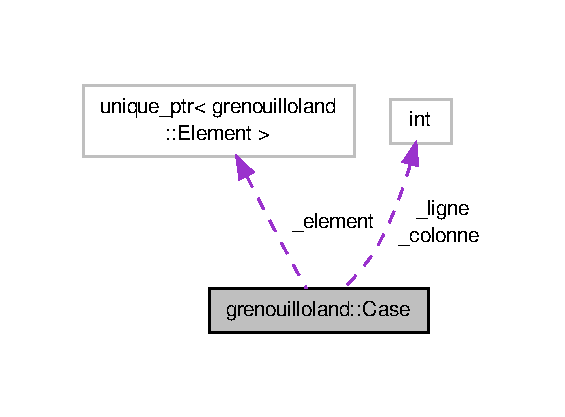
\includegraphics[width=271pt]{classgrenouilloland_1_1Case__coll__graph}
\end{center}
\end{figure}
\subsection*{Fonctions membres publiques}
\begin{DoxyCompactItemize}
\item 
\hyperlink{classgrenouilloland_1_1Case_a70869d260d32a037b2f72b56990abc42}{Case} (const int \&colonne, const int \&ligne)
\item 
const int \& \hyperlink{classgrenouilloland_1_1Case_aedf4adbcb065ba1f3d178dccd0a54679}{lire\-Ligne} () const 
\item 
const int \& \hyperlink{classgrenouilloland_1_1Case_a58ddf443efa9e649e9a9e61b019ec3b8}{lire\-Colonne} () const 
\item 
const \hyperlink{classgrenouilloland_1_1Element}{Element} \& \hyperlink{classgrenouilloland_1_1Case_a823dafb736c38d71b6a3192cd6a3d0fd}{lire\-Element} () const 
\end{DoxyCompactItemize}
\subsection*{Fonctions membres protégées}
\begin{DoxyCompactItemize}
\item 
void \hyperlink{classgrenouilloland_1_1Case_ab57246e24672017b0cb29484ca6d2921}{changer\-Element} (\hyperlink{classgrenouilloland_1_1Element}{Element} $\ast$element)
\item 
\hyperlink{classgrenouilloland_1_1Etat}{Etat} \hyperlink{classgrenouilloland_1_1Case_a9e746c0dba7c7bcf166ca88bb10d9b01}{vieillir\-Element} ()
\end{DoxyCompactItemize}
\subsection*{Attributs protégés}
\begin{DoxyCompactItemize}
\item 
int \hyperlink{classgrenouilloland_1_1Case_a852142435ab4a556c148274cccbcfebc}{\-\_\-ligne}
\item 
int \hyperlink{classgrenouilloland_1_1Case_a44c61a8ab51a6fedb92c9a92c7eeb9eb}{\-\_\-colonne}
\item 
std\-::unique\-\_\-ptr$<$ \hyperlink{classgrenouilloland_1_1Element}{Element} $>$ \hyperlink{classgrenouilloland_1_1Case_a3ffd88341a2aee34d145ddf5a986ab37}{\-\_\-element}
\end{DoxyCompactItemize}
\subsection*{Amis}
\begin{DoxyCompactItemize}
\item 
\hypertarget{classgrenouilloland_1_1Case_a8347c819d94b3816d06cf9255691923d}{class {\bfseries Jeu}}\label{classgrenouilloland_1_1Case_a8347c819d94b3816d06cf9255691923d}

\end{DoxyCompactItemize}


\subsection{Description détaillée}
\hyperlink{classgrenouilloland_1_1Case}{Case} du \hyperlink{classgrenouilloland_1_1Jeu}{Jeu} Grenouilloland. 

\begin{DoxyAuthor}{Auteur}
Beudin Alexandre -\/ Dauxais Yann 
\end{DoxyAuthor}
\begin{DoxyDate}{Date}
05.\-01.\-2012
\end{DoxyDate}
Declaration de la classe \hyperlink{classgrenouilloland_1_1Case}{Case} representant une \hyperlink{classgrenouilloland_1_1Case}{Case} du \hyperlink{classgrenouilloland_1_1Jeu}{Jeu} Grenouilloland. 

\subsection{Documentation des constructeurs et destructeur}
\hypertarget{classgrenouilloland_1_1Case_a70869d260d32a037b2f72b56990abc42}{\index{grenouilloland\-::\-Case@{grenouilloland\-::\-Case}!Case@{Case}}
\index{Case@{Case}!grenouilloland::Case@{grenouilloland\-::\-Case}}
\subsubsection[{Case}]{\setlength{\rightskip}{0pt plus 5cm}Case\-::\-Case (
\begin{DoxyParamCaption}
\item[{const int \&}]{colonne, }
\item[{const int \&}]{ligne}
\end{DoxyParamCaption}
)}}\label{classgrenouilloland_1_1Case_a70869d260d32a037b2f72b56990abc42}
Constructeur logique instanciant une case.


\begin{DoxyParams}[1]{Paramètres}
\mbox{\tt in}  & {\em colonne} & -\/ la valeur de \hyperlink{classgrenouilloland_1_1Case_a44c61a8ab51a6fedb92c9a92c7eeb9eb}{\-\_\-colonne}. \\
\hline
\mbox{\tt in}  & {\em ligne} & -\/ la valeur de \hyperlink{classgrenouilloland_1_1Case_a852142435ab4a556c148274cccbcfebc}{\-\_\-ligne}. \\
\hline
\end{DoxyParams}


\subsection{Documentation des fonctions membres}
\hypertarget{classgrenouilloland_1_1Case_ab57246e24672017b0cb29484ca6d2921}{\index{grenouilloland\-::\-Case@{grenouilloland\-::\-Case}!changer\-Element@{changer\-Element}}
\index{changer\-Element@{changer\-Element}!grenouilloland::Case@{grenouilloland\-::\-Case}}
\subsubsection[{changer\-Element}]{\setlength{\rightskip}{0pt plus 5cm}void Case\-::changer\-Element (
\begin{DoxyParamCaption}
\item[{{\bf Element} $\ast$}]{element}
\end{DoxyParamCaption}
)\hspace{0.3cm}{\ttfamily [protected]}}}\label{classgrenouilloland_1_1Case_ab57246e24672017b0cb29484ca6d2921}
Remplace l'élement présent par celui en paramètre.


\begin{DoxyParams}[1]{Paramètres}
\mbox{\tt in,out}  & {\em element} & -\/ nouvel élément de la cellule. \\
\hline
\end{DoxyParams}
\hypertarget{classgrenouilloland_1_1Case_a58ddf443efa9e649e9a9e61b019ec3b8}{\index{grenouilloland\-::\-Case@{grenouilloland\-::\-Case}!lire\-Colonne@{lire\-Colonne}}
\index{lire\-Colonne@{lire\-Colonne}!grenouilloland::Case@{grenouilloland\-::\-Case}}
\subsubsection[{lire\-Colonne}]{\setlength{\rightskip}{0pt plus 5cm}const int \& Case\-::lire\-Colonne (
\begin{DoxyParamCaption}
{}
\end{DoxyParamCaption}
) const}}\label{classgrenouilloland_1_1Case_a58ddf443efa9e649e9a9e61b019ec3b8}
Accesseur du numéro de colonne.

\begin{DoxyReturn}{Renvoie}
la valeur de \hyperlink{classgrenouilloland_1_1Case_a44c61a8ab51a6fedb92c9a92c7eeb9eb}{\-\_\-colonne}. 
\end{DoxyReturn}
\hypertarget{classgrenouilloland_1_1Case_a823dafb736c38d71b6a3192cd6a3d0fd}{\index{grenouilloland\-::\-Case@{grenouilloland\-::\-Case}!lire\-Element@{lire\-Element}}
\index{lire\-Element@{lire\-Element}!grenouilloland::Case@{grenouilloland\-::\-Case}}
\subsubsection[{lire\-Element}]{\setlength{\rightskip}{0pt plus 5cm}const {\bf Element} \& Case\-::lire\-Element (
\begin{DoxyParamCaption}
{}
\end{DoxyParamCaption}
) const}}\label{classgrenouilloland_1_1Case_a823dafb736c38d71b6a3192cd6a3d0fd}
Accesseur de l'élément.

\begin{DoxyReturn}{Renvoie}
la valeur de l'élément pointé par \hyperlink{classgrenouilloland_1_1Case_a3ffd88341a2aee34d145ddf5a986ab37}{\-\_\-element}. 
\end{DoxyReturn}
\hypertarget{classgrenouilloland_1_1Case_aedf4adbcb065ba1f3d178dccd0a54679}{\index{grenouilloland\-::\-Case@{grenouilloland\-::\-Case}!lire\-Ligne@{lire\-Ligne}}
\index{lire\-Ligne@{lire\-Ligne}!grenouilloland::Case@{grenouilloland\-::\-Case}}
\subsubsection[{lire\-Ligne}]{\setlength{\rightskip}{0pt plus 5cm}const int \& Case\-::lire\-Ligne (
\begin{DoxyParamCaption}
{}
\end{DoxyParamCaption}
) const}}\label{classgrenouilloland_1_1Case_aedf4adbcb065ba1f3d178dccd0a54679}
Accesseur du numéro de ligne.

\begin{DoxyReturn}{Renvoie}
la valeur de \hyperlink{classgrenouilloland_1_1Case_a852142435ab4a556c148274cccbcfebc}{\-\_\-ligne}. 
\end{DoxyReturn}
\hypertarget{classgrenouilloland_1_1Case_a9e746c0dba7c7bcf166ca88bb10d9b01}{\index{grenouilloland\-::\-Case@{grenouilloland\-::\-Case}!vieillir\-Element@{vieillir\-Element}}
\index{vieillir\-Element@{vieillir\-Element}!grenouilloland::Case@{grenouilloland\-::\-Case}}
\subsubsection[{vieillir\-Element}]{\setlength{\rightskip}{0pt plus 5cm}{\bf Etat} Case\-::vieillir\-Element (
\begin{DoxyParamCaption}
{}
\end{DoxyParamCaption}
)\hspace{0.3cm}{\ttfamily [protected]}}}\label{classgrenouilloland_1_1Case_a9e746c0dba7c7bcf166ca88bb10d9b01}
Vieillisement de l'élément.

\begin{DoxyReturn}{Renvoie}
nouvel état de l'élément pointé par \hyperlink{classgrenouilloland_1_1Case_a3ffd88341a2aee34d145ddf5a986ab37}{\-\_\-element}. 
\end{DoxyReturn}


\subsection{Documentation des données membres}
\hypertarget{classgrenouilloland_1_1Case_a44c61a8ab51a6fedb92c9a92c7eeb9eb}{\index{grenouilloland\-::\-Case@{grenouilloland\-::\-Case}!\-\_\-colonne@{\-\_\-colonne}}
\index{\-\_\-colonne@{\-\_\-colonne}!grenouilloland::Case@{grenouilloland\-::\-Case}}
\subsubsection[{\-\_\-colonne}]{\setlength{\rightskip}{0pt plus 5cm}int grenouilloland\-::\-Case\-::\-\_\-colonne\hspace{0.3cm}{\ttfamily [protected]}}}\label{classgrenouilloland_1_1Case_a44c61a8ab51a6fedb92c9a92c7eeb9eb}
Numero de colonne de cette cellule. \hypertarget{classgrenouilloland_1_1Case_a3ffd88341a2aee34d145ddf5a986ab37}{\index{grenouilloland\-::\-Case@{grenouilloland\-::\-Case}!\-\_\-element@{\-\_\-element}}
\index{\-\_\-element@{\-\_\-element}!grenouilloland::Case@{grenouilloland\-::\-Case}}
\subsubsection[{\-\_\-element}]{\setlength{\rightskip}{0pt plus 5cm}std\-::unique\-\_\-ptr$<${\bf Element}$>$ grenouilloland\-::\-Case\-::\-\_\-element\hspace{0.3cm}{\ttfamily [protected]}}}\label{classgrenouilloland_1_1Case_a3ffd88341a2aee34d145ddf5a986ab37}
\hyperlink{classgrenouilloland_1_1Element}{Element} contenu dans la cellule. \hypertarget{classgrenouilloland_1_1Case_a852142435ab4a556c148274cccbcfebc}{\index{grenouilloland\-::\-Case@{grenouilloland\-::\-Case}!\-\_\-ligne@{\-\_\-ligne}}
\index{\-\_\-ligne@{\-\_\-ligne}!grenouilloland::Case@{grenouilloland\-::\-Case}}
\subsubsection[{\-\_\-ligne}]{\setlength{\rightskip}{0pt plus 5cm}int grenouilloland\-::\-Case\-::\-\_\-ligne\hspace{0.3cm}{\ttfamily [protected]}}}\label{classgrenouilloland_1_1Case_a852142435ab4a556c148274cccbcfebc}
Numero de ligne de cette cellule. 

La documentation de cette classe a été générée à partir des fichiers suivants \-:\begin{DoxyCompactItemize}
\item 
src/modele/include/Case.\-hh\item 
src/modele/Case.\-cpp\end{DoxyCompactItemize}

\hypertarget{classgrenouilloland_1_1CaseGraphique}{\section{Référence de la classe grenouilloland\-:\-:Case\-Graphique}
\label{classgrenouilloland_1_1CaseGraphique}\index{grenouilloland\-::\-Case\-Graphique@{grenouilloland\-::\-Case\-Graphique}}
}


Representation graphique d'une \hyperlink{classgrenouilloland_1_1Case}{Case}.  




{\ttfamily \#include $<$Case\-Graphique.\-hh$>$}



Graphe d'héritage de grenouilloland\-:\-:Case\-Graphique\-:
\nopagebreak
\begin{figure}[H]
\begin{center}
\leavevmode
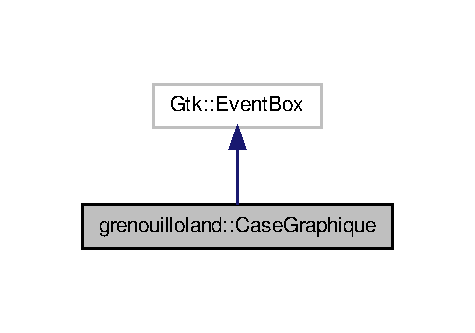
\includegraphics[width=228pt]{classgrenouilloland_1_1CaseGraphique__inherit__graph}
\end{center}
\end{figure}


Graphe de collaboration de grenouilloland\-:\-:Case\-Graphique\-:
\nopagebreak
\begin{figure}[H]
\begin{center}
\leavevmode
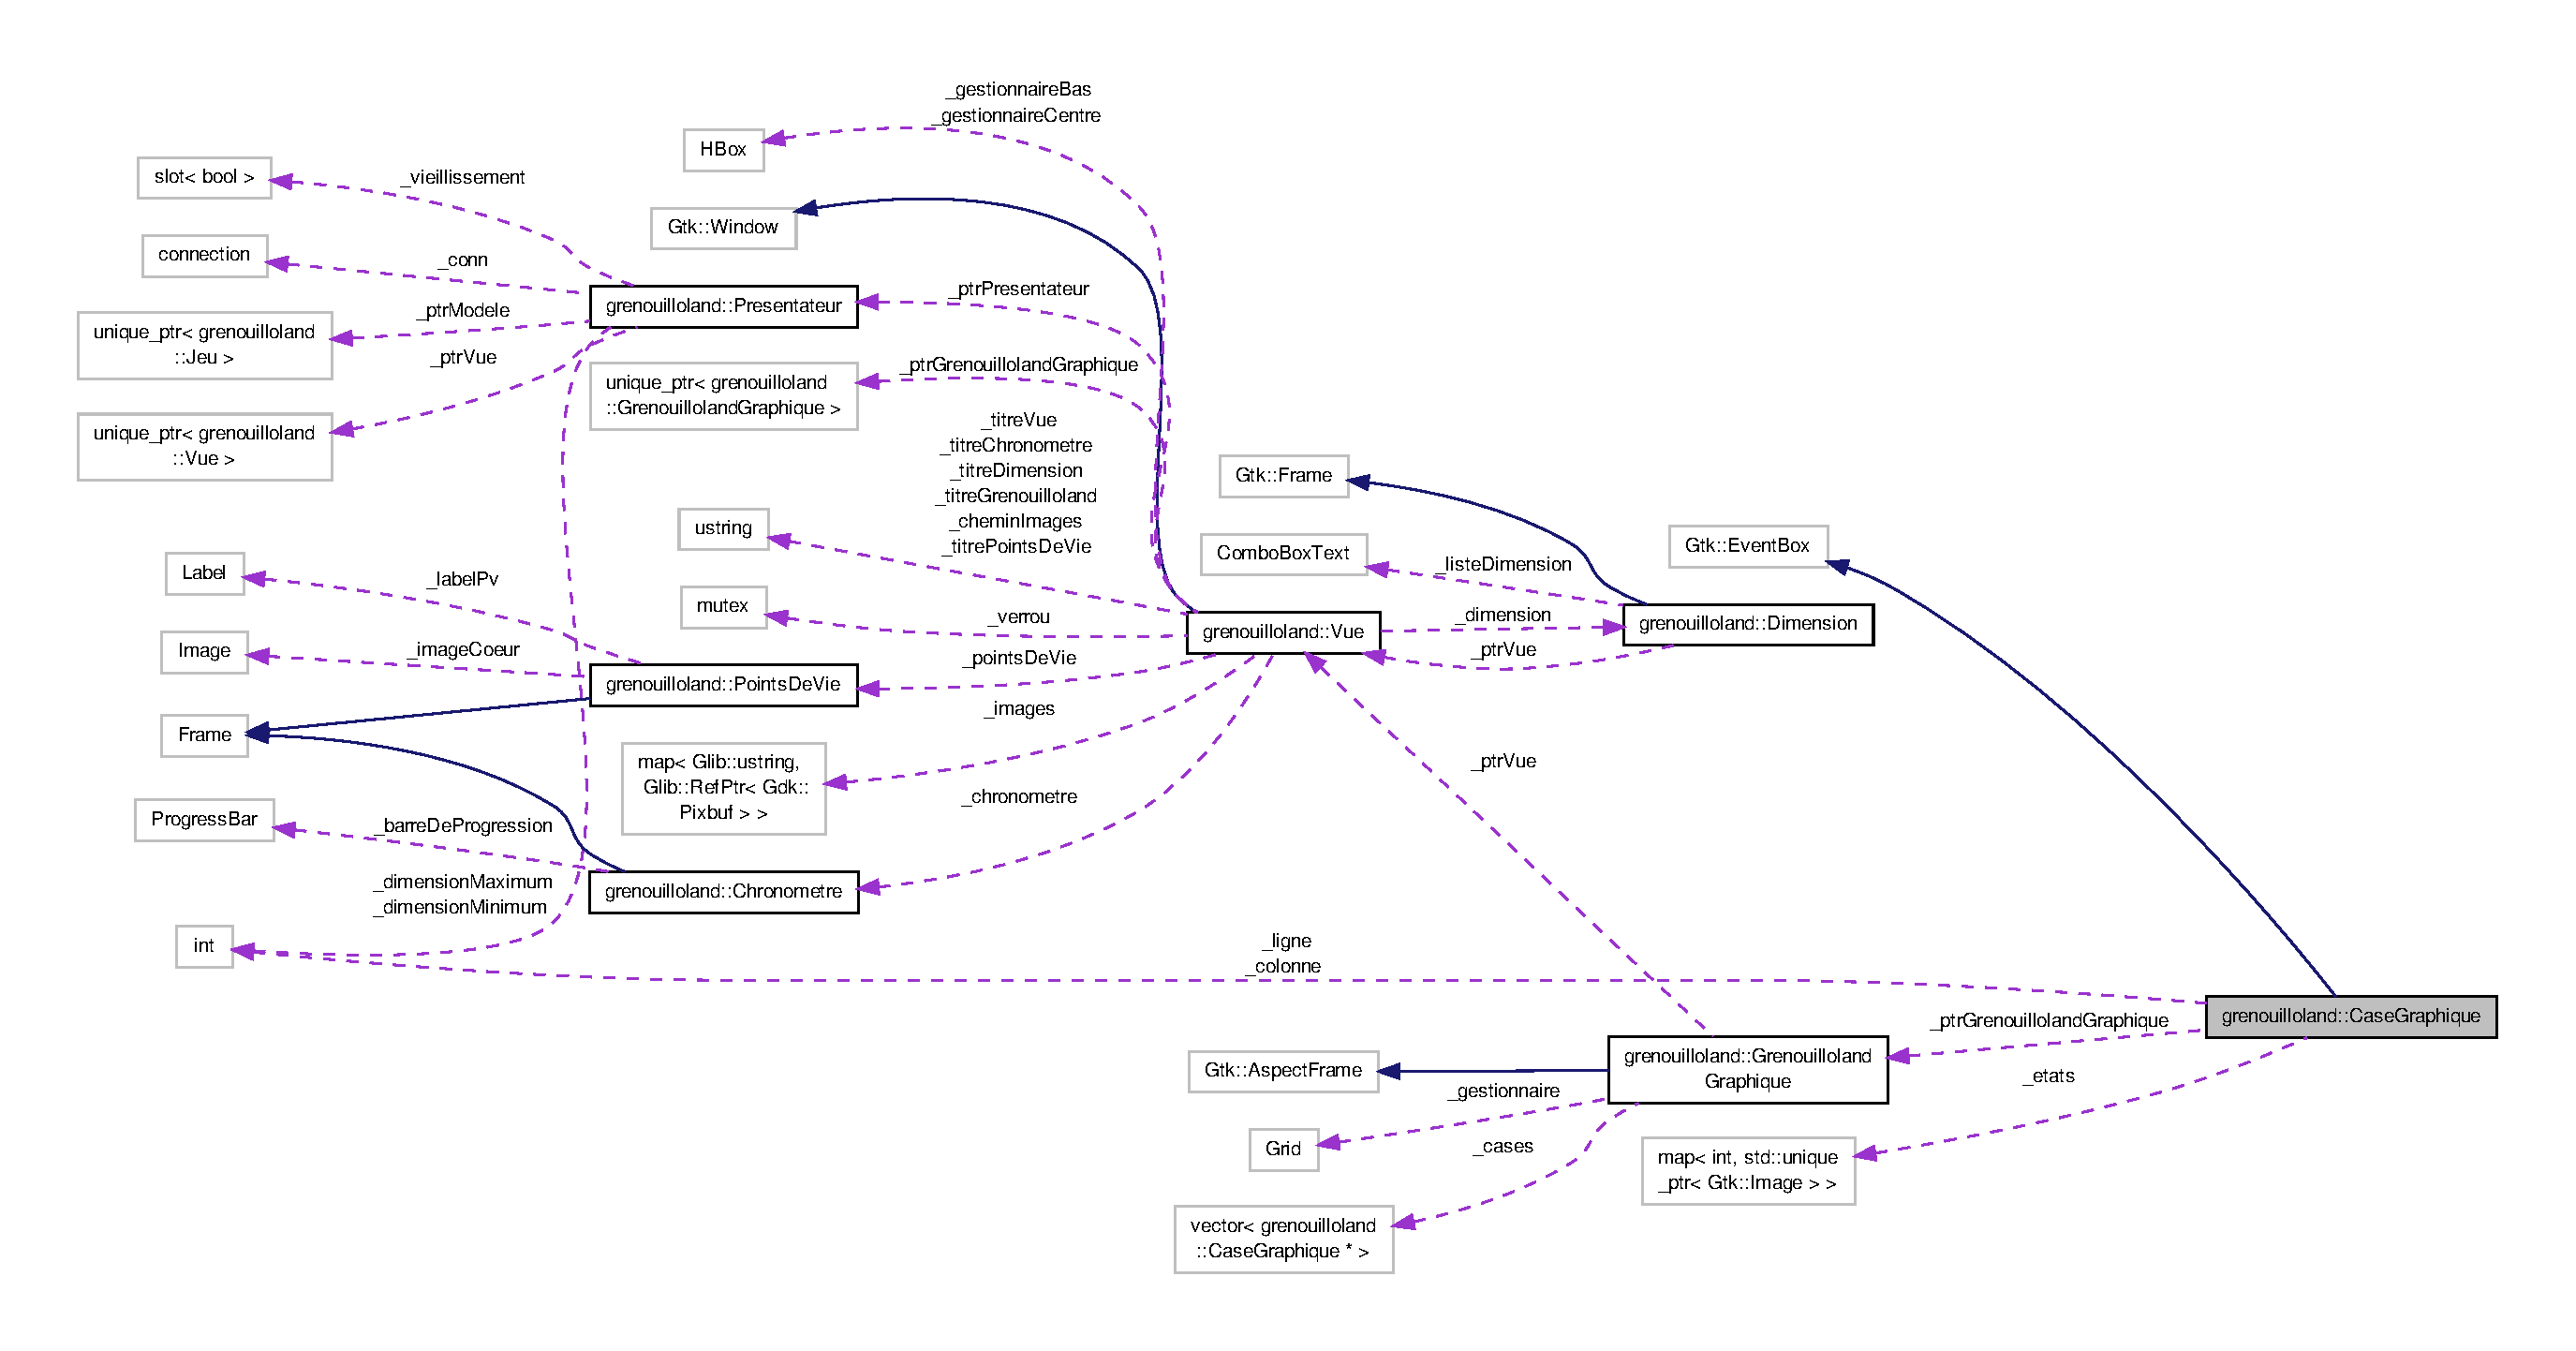
\includegraphics[width=350pt]{classgrenouilloland_1_1CaseGraphique__coll__graph}
\end{center}
\end{figure}
\subsection*{Fonctions membres publiques}
\begin{DoxyCompactItemize}
\item 
\hyperlink{classgrenouilloland_1_1CaseGraphique_a05e456185c11de9239e27bff41c2d53e}{Case\-Graphique} (\hyperlink{classgrenouilloland_1_1GrenouillolandGraphique}{Grenouilloland\-Graphique} \&grenouilloland\-Graphique, const int \&colonne, const int \&ligne)
\item 
const \hyperlink{classgrenouilloland_1_1GrenouillolandGraphique}{Grenouilloland\-Graphique} \& \hyperlink{classgrenouilloland_1_1CaseGraphique_a10c9a3768da212d67598deda0609d98f}{lire\-Grenouilloland\-Graphique} () const 
\item 
const int \& \hyperlink{classgrenouilloland_1_1CaseGraphique_a0533ed9960cdd84cdc064888cc27d952}{lire\-Ligne} () const 
\item 
const int \& \hyperlink{classgrenouilloland_1_1CaseGraphique_a8f575954b15de168325c0869c66d6a87}{lire\-Colonne} () const 
\end{DoxyCompactItemize}
\subsection*{Fonctions membres protégées}
\begin{DoxyCompactItemize}
\item 
void \hyperlink{classgrenouilloland_1_1CaseGraphique_a08a0e069b5572708c69beb22edc6da65}{mettre\-A\-Jour} (const \hyperlink{classgrenouilloland_1_1Presentateur}{Presentateur} \&presentateur)
\item 
bool \hyperlink{classgrenouilloland_1_1CaseGraphique_ab6f2daebfafae5076c4390ecbed5cbe1}{cb\-Click\-Souris} (Gdk\-Event\-Button $\ast$evt)
\end{DoxyCompactItemize}
\subsection*{Attributs protégés}
\begin{DoxyCompactItemize}
\item 
\hyperlink{classgrenouilloland_1_1GrenouillolandGraphique}{Grenouilloland\-Graphique} $\ast$const \hyperlink{classgrenouilloland_1_1CaseGraphique_a0ef536735e07c4f90f32afa4b74928d3}{\-\_\-ptr\-Grenouilloland\-Graphique}
\item 
const int \hyperlink{classgrenouilloland_1_1CaseGraphique_a66f59a2fcbc16ffda0bd1e30471737f3}{\-\_\-ligne}
\item 
const int \hyperlink{classgrenouilloland_1_1CaseGraphique_ae4e49cd04cefb12a3b42e2e57678520a}{\-\_\-colonne}
\item 
std\-::map$<$ int, std\-::unique\-\_\-ptr\\*
$<$ Gtk\-::\-Image $>$ $>$ \hyperlink{classgrenouilloland_1_1CaseGraphique_a020fe5a8b0c1e7d803c50ba268ec83d7}{\-\_\-etats}
\end{DoxyCompactItemize}
\subsection*{Amis}
\begin{DoxyCompactItemize}
\item 
class \hyperlink{classgrenouilloland_1_1CaseGraphique_afaa793860facc1cb19fbc6b54b38c4f8}{Grenouilloland\-Graphique}
\end{DoxyCompactItemize}


\subsection{Description détaillée}
Representation graphique d'une \hyperlink{classgrenouilloland_1_1Case}{Case}. 

\begin{DoxyAuthor}{Auteur}
Yann Dauxais 

Alexandre Beudin 
\end{DoxyAuthor}
\begin{DoxyDate}{Date}
6.\-1.\-2013
\end{DoxyDate}
Declaration de la classe \hyperlink{classgrenouilloland_1_1CaseGraphique}{Case\-Graphique} representant graphiquement une case du modele.

\begin{DoxyNote}{Note}
Une instance de cette classe ne peut être dupliquée. L'operateur d'affectation est naturellement et implicitement retire car deux des attributs de cette classe sont des constantes.

Chaque instance de cette classe est son propre listener. 
\end{DoxyNote}


\subsection{Documentation des constructeurs et destructeur}
\hypertarget{classgrenouilloland_1_1CaseGraphique_a05e456185c11de9239e27bff41c2d53e}{\index{grenouilloland\-::\-Case\-Graphique@{grenouilloland\-::\-Case\-Graphique}!Case\-Graphique@{Case\-Graphique}}
\index{Case\-Graphique@{Case\-Graphique}!grenouilloland::CaseGraphique@{grenouilloland\-::\-Case\-Graphique}}
\subsubsection[{Case\-Graphique}]{\setlength{\rightskip}{0pt plus 5cm}Case\-Graphique\-::\-Case\-Graphique (
\begin{DoxyParamCaption}
\item[{{\bf Grenouilloland\-Graphique} \&}]{grenouilloland\-Graphique, }
\item[{const int \&}]{colonne, }
\item[{const int \&}]{ligne}
\end{DoxyParamCaption}
)}}\label{classgrenouilloland_1_1CaseGraphique_a05e456185c11de9239e27bff41c2d53e}
Constructeur logique.


\begin{DoxyParams}[1]{Paramètres}
\mbox{\tt in,out}  & {\em jeu} & -\/ la valeur de \hyperlink{classgrenouilloland_1_1CaseGraphique_a0ef536735e07c4f90f32afa4b74928d3}{\-\_\-ptr\-Grenouilloland\-Graphique}. \\
\hline
\mbox{\tt in}  & {\em ligne} & -\/ la valeur de \hyperlink{classgrenouilloland_1_1CaseGraphique_a66f59a2fcbc16ffda0bd1e30471737f3}{\-\_\-ligne}. \\
\hline
\mbox{\tt in}  & {\em colonne} & -\/ la valeur de \hyperlink{classgrenouilloland_1_1CaseGraphique_ae4e49cd04cefb12a3b42e2e57678520a}{\-\_\-colonne}. \\
\hline
\end{DoxyParams}


\subsection{Documentation des fonctions membres}
\hypertarget{classgrenouilloland_1_1CaseGraphique_ab6f2daebfafae5076c4390ecbed5cbe1}{\index{grenouilloland\-::\-Case\-Graphique@{grenouilloland\-::\-Case\-Graphique}!cb\-Click\-Souris@{cb\-Click\-Souris}}
\index{cb\-Click\-Souris@{cb\-Click\-Souris}!grenouilloland::CaseGraphique@{grenouilloland\-::\-Case\-Graphique}}
\subsubsection[{cb\-Click\-Souris}]{\setlength{\rightskip}{0pt plus 5cm}bool Case\-Graphique\-::cb\-Click\-Souris (
\begin{DoxyParamCaption}
\item[{Gdk\-Event\-Button $\ast$}]{evt}
\end{DoxyParamCaption}
)\hspace{0.3cm}{\ttfamily [protected]}}}\label{classgrenouilloland_1_1CaseGraphique_ab6f2daebfafae5076c4390ecbed5cbe1}
Callback invoque lors d'un click de souris sur cette case graphique.


\begin{DoxyParams}[1]{Paramètres}
\mbox{\tt in}  & {\em evt} & -\/ l'evenement associe au click. \\
\hline
\end{DoxyParams}
\begin{DoxyReturn}{Renvoie}
la valeur {\ttfamily true}. 
\end{DoxyReturn}
\hypertarget{classgrenouilloland_1_1CaseGraphique_a8f575954b15de168325c0869c66d6a87}{\index{grenouilloland\-::\-Case\-Graphique@{grenouilloland\-::\-Case\-Graphique}!lire\-Colonne@{lire\-Colonne}}
\index{lire\-Colonne@{lire\-Colonne}!grenouilloland::CaseGraphique@{grenouilloland\-::\-Case\-Graphique}}
\subsubsection[{lire\-Colonne}]{\setlength{\rightskip}{0pt plus 5cm}const int \& Case\-Graphique\-::lire\-Colonne (
\begin{DoxyParamCaption}
{}
\end{DoxyParamCaption}
) const}}\label{classgrenouilloland_1_1CaseGraphique_a8f575954b15de168325c0869c66d6a87}
Accesseur.

\begin{DoxyReturn}{Renvoie}
la valeur de \hyperlink{classgrenouilloland_1_1CaseGraphique_ae4e49cd04cefb12a3b42e2e57678520a}{\-\_\-colonne}. 
\end{DoxyReturn}
\hypertarget{classgrenouilloland_1_1CaseGraphique_a10c9a3768da212d67598deda0609d98f}{\index{grenouilloland\-::\-Case\-Graphique@{grenouilloland\-::\-Case\-Graphique}!lire\-Grenouilloland\-Graphique@{lire\-Grenouilloland\-Graphique}}
\index{lire\-Grenouilloland\-Graphique@{lire\-Grenouilloland\-Graphique}!grenouilloland::CaseGraphique@{grenouilloland\-::\-Case\-Graphique}}
\subsubsection[{lire\-Grenouilloland\-Graphique}]{\setlength{\rightskip}{0pt plus 5cm}const {\bf Grenouilloland\-Graphique} \& Case\-Graphique\-::lire\-Grenouilloland\-Graphique (
\begin{DoxyParamCaption}
{}
\end{DoxyParamCaption}
) const}}\label{classgrenouilloland_1_1CaseGraphique_a10c9a3768da212d67598deda0609d98f}
Accesseur.

\begin{DoxyReturn}{Renvoie}
la valeur de \hyperlink{classgrenouilloland_1_1CaseGraphique_a0ef536735e07c4f90f32afa4b74928d3}{\-\_\-ptr\-Grenouilloland\-Graphique}. 
\end{DoxyReturn}
\hypertarget{classgrenouilloland_1_1CaseGraphique_a0533ed9960cdd84cdc064888cc27d952}{\index{grenouilloland\-::\-Case\-Graphique@{grenouilloland\-::\-Case\-Graphique}!lire\-Ligne@{lire\-Ligne}}
\index{lire\-Ligne@{lire\-Ligne}!grenouilloland::CaseGraphique@{grenouilloland\-::\-Case\-Graphique}}
\subsubsection[{lire\-Ligne}]{\setlength{\rightskip}{0pt plus 5cm}const int \& Case\-Graphique\-::lire\-Ligne (
\begin{DoxyParamCaption}
{}
\end{DoxyParamCaption}
) const}}\label{classgrenouilloland_1_1CaseGraphique_a0533ed9960cdd84cdc064888cc27d952}
Accesseur.

\begin{DoxyReturn}{Renvoie}
la valeur de \hyperlink{classgrenouilloland_1_1CaseGraphique_a66f59a2fcbc16ffda0bd1e30471737f3}{\-\_\-ligne}. 
\end{DoxyReturn}
\hypertarget{classgrenouilloland_1_1CaseGraphique_a08a0e069b5572708c69beb22edc6da65}{\index{grenouilloland\-::\-Case\-Graphique@{grenouilloland\-::\-Case\-Graphique}!mettre\-A\-Jour@{mettre\-A\-Jour}}
\index{mettre\-A\-Jour@{mettre\-A\-Jour}!grenouilloland::CaseGraphique@{grenouilloland\-::\-Case\-Graphique}}
\subsubsection[{mettre\-A\-Jour}]{\setlength{\rightskip}{0pt plus 5cm}void Case\-Graphique\-::mettre\-A\-Jour (
\begin{DoxyParamCaption}
\item[{const {\bf Presentateur} \&}]{presentateur}
\end{DoxyParamCaption}
)\hspace{0.3cm}{\ttfamily [protected]}}}\label{classgrenouilloland_1_1CaseGraphique_a08a0e069b5572708c69beb22edc6da65}
Demande a cette case graphique de se mettre a jour en fonction de l'etat de la case correspondante du modele.


\begin{DoxyParams}[1]{Paramètres}
\mbox{\tt in}  & {\em presentateur} & -\/ le presentateur a invoquer.\\
\hline
\end{DoxyParams}
\begin{DoxyNote}{Note}
La vue doit etre verrouille pour pouvoir invoquer cette methode. 
\end{DoxyNote}


\subsection{Documentation des fonctions amies et associées}
\hypertarget{classgrenouilloland_1_1CaseGraphique_afaa793860facc1cb19fbc6b54b38c4f8}{\index{grenouilloland\-::\-Case\-Graphique@{grenouilloland\-::\-Case\-Graphique}!Grenouilloland\-Graphique@{Grenouilloland\-Graphique}}
\index{Grenouilloland\-Graphique@{Grenouilloland\-Graphique}!grenouilloland::CaseGraphique@{grenouilloland\-::\-Case\-Graphique}}
\subsubsection[{Grenouilloland\-Graphique}]{\setlength{\rightskip}{0pt plus 5cm}friend class {\bf Grenouilloland\-Graphique}\hspace{0.3cm}{\ttfamily [friend]}}}\label{classgrenouilloland_1_1CaseGraphique_afaa793860facc1cb19fbc6b54b38c4f8}
Declaration d'amitié. 

\subsection{Documentation des données membres}
\hypertarget{classgrenouilloland_1_1CaseGraphique_ae4e49cd04cefb12a3b42e2e57678520a}{\index{grenouilloland\-::\-Case\-Graphique@{grenouilloland\-::\-Case\-Graphique}!\-\_\-colonne@{\-\_\-colonne}}
\index{\-\_\-colonne@{\-\_\-colonne}!grenouilloland::CaseGraphique@{grenouilloland\-::\-Case\-Graphique}}
\subsubsection[{\-\_\-colonne}]{\setlength{\rightskip}{0pt plus 5cm}const int grenouilloland\-::\-Case\-Graphique\-::\-\_\-colonne\hspace{0.3cm}{\ttfamily [protected]}}}\label{classgrenouilloland_1_1CaseGraphique_ae4e49cd04cefb12a3b42e2e57678520a}
Numero de colonne de cette case dans le modele. \hypertarget{classgrenouilloland_1_1CaseGraphique_a020fe5a8b0c1e7d803c50ba268ec83d7}{\index{grenouilloland\-::\-Case\-Graphique@{grenouilloland\-::\-Case\-Graphique}!\-\_\-etats@{\-\_\-etats}}
\index{\-\_\-etats@{\-\_\-etats}!grenouilloland::CaseGraphique@{grenouilloland\-::\-Case\-Graphique}}
\subsubsection[{\-\_\-etats}]{\setlength{\rightskip}{0pt plus 5cm}std\-::map$<$ int, std\-::unique\-\_\-ptr$<$ Gtk\-::\-Image $>$ $>$ grenouilloland\-::\-Case\-Graphique\-::\-\_\-etats\hspace{0.3cm}{\ttfamily [protected]}}}\label{classgrenouilloland_1_1CaseGraphique_a020fe5a8b0c1e7d803c50ba268ec83d7}
Pixmaps representant les etats possibles d'une case graphique.

\begin{DoxyNote}{Note}
En toute rigueur, cette map devrait etre definie en tant qu'attribut de classe et non d'instance. Cependant, G\-T\-K ne supporte pas qu'un widget puisse appartenir a plusieurs container. Par consequent, nous devons repliquer les images, d'ou un gaspillage de memoire. 
\end{DoxyNote}
\hypertarget{classgrenouilloland_1_1CaseGraphique_a66f59a2fcbc16ffda0bd1e30471737f3}{\index{grenouilloland\-::\-Case\-Graphique@{grenouilloland\-::\-Case\-Graphique}!\-\_\-ligne@{\-\_\-ligne}}
\index{\-\_\-ligne@{\-\_\-ligne}!grenouilloland::CaseGraphique@{grenouilloland\-::\-Case\-Graphique}}
\subsubsection[{\-\_\-ligne}]{\setlength{\rightskip}{0pt plus 5cm}const int grenouilloland\-::\-Case\-Graphique\-::\-\_\-ligne\hspace{0.3cm}{\ttfamily [protected]}}}\label{classgrenouilloland_1_1CaseGraphique_a66f59a2fcbc16ffda0bd1e30471737f3}
Numero de ligne de cette case dans le modele. \hypertarget{classgrenouilloland_1_1CaseGraphique_a0ef536735e07c4f90f32afa4b74928d3}{\index{grenouilloland\-::\-Case\-Graphique@{grenouilloland\-::\-Case\-Graphique}!\-\_\-ptr\-Grenouilloland\-Graphique@{\-\_\-ptr\-Grenouilloland\-Graphique}}
\index{\-\_\-ptr\-Grenouilloland\-Graphique@{\-\_\-ptr\-Grenouilloland\-Graphique}!grenouilloland::CaseGraphique@{grenouilloland\-::\-Case\-Graphique}}
\subsubsection[{\-\_\-ptr\-Grenouilloland\-Graphique}]{\setlength{\rightskip}{0pt plus 5cm}{\bf Grenouilloland\-Graphique}$\ast$ const grenouilloland\-::\-Case\-Graphique\-::\-\_\-ptr\-Grenouilloland\-Graphique\hspace{0.3cm}{\ttfamily [protected]}}}\label{classgrenouilloland_1_1CaseGraphique_a0ef536735e07c4f90f32afa4b74928d3}
Unique representation graphique du jeu proprietaire de cette case graphique. 

La documentation de cette classe a été générée à partir des fichiers suivants \-:\begin{DoxyCompactItemize}
\item 
src/vue/include/Case\-Graphique.\-hh\item 
src/vue/Case\-Graphique.\-cpp\end{DoxyCompactItemize}

\hypertarget{classgrenouilloland_1_1Chronometre}{\section{Référence de la classe grenouilloland\-:\-:Chronometre}
\label{classgrenouilloland_1_1Chronometre}\index{grenouilloland\-::\-Chronometre@{grenouilloland\-::\-Chronometre}}
}


Afficheur du temps de \hyperlink{classgrenouilloland_1_1Jeu}{Jeu}.  




{\ttfamily \#include $<$Chronometre.\-hh$>$}



Graphe d'héritage de grenouilloland\-:\-:Chronometre\-:
\nopagebreak
\begin{figure}[H]
\begin{center}
\leavevmode
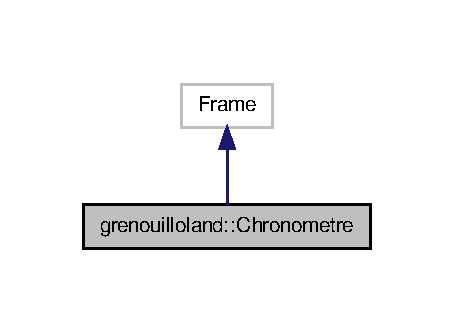
\includegraphics[width=218pt]{classgrenouilloland_1_1Chronometre__inherit__graph}
\end{center}
\end{figure}


Graphe de collaboration de grenouilloland\-:\-:Chronometre\-:
\nopagebreak
\begin{figure}[H]
\begin{center}
\leavevmode
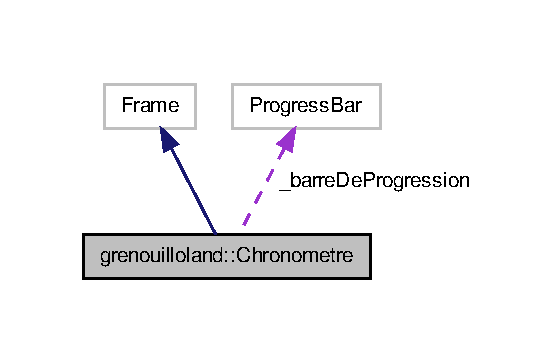
\includegraphics[width=266pt]{classgrenouilloland_1_1Chronometre__coll__graph}
\end{center}
\end{figure}
\subsection*{Fonctions membres publiques}
\begin{DoxyCompactItemize}
\item 
\hyperlink{classgrenouilloland_1_1Chronometre_a7331d6bd863468b99f501c9ef72f3d18}{Chronometre} (const Glib\-::ustring \&titre)
\end{DoxyCompactItemize}
\subsection*{Fonctions membres protégées}
\begin{DoxyCompactItemize}
\item 
void \hyperlink{classgrenouilloland_1_1Chronometre_ac7b8f9ef96571fdda6f3a328aec1db8d}{mettre\-A\-Jour} (const \hyperlink{classgrenouilloland_1_1Presentateur}{Presentateur} \&presentateur)
\end{DoxyCompactItemize}
\subsection*{Attributs protégés}
\begin{DoxyCompactItemize}
\item 
Gtk\-::\-Progress\-Bar \hyperlink{classgrenouilloland_1_1Chronometre_a0d69d261d1caf45e33f310cbc3132d6d}{\-\_\-barre\-De\-Progression}
\end{DoxyCompactItemize}
\subsection*{Amis}
\begin{DoxyCompactItemize}
\item 
class \hyperlink{classgrenouilloland_1_1Chronometre_adc3b1810b8d3988a7832f57c330fe4fd}{Vue}
\end{DoxyCompactItemize}


\subsection{Description détaillée}
Afficheur du temps de \hyperlink{classgrenouilloland_1_1Jeu}{Jeu}. 

\begin{DoxyAuthor}{Auteur}
Yann Dauxais 

Alexandre Beudin 
\end{DoxyAuthor}
\begin{DoxyDate}{Date}
6.\-1.\-2013
\end{DoxyDate}
Declaration de la classe \hyperlink{classgrenouilloland_1_1Chronometre}{Chronometre} representant l'affichage du chronomètre du \hyperlink{classgrenouilloland_1_1Jeu}{Jeu}. Le Widget utilisé est une barre de progression.

\begin{DoxyNote}{Note}
une instance de cette classe ne peut etre dupliquee.

chaque instance de cette classe est son propre listener. 
\end{DoxyNote}


\subsection{Documentation des constructeurs et destructeur}
\hypertarget{classgrenouilloland_1_1Chronometre_a7331d6bd863468b99f501c9ef72f3d18}{\index{grenouilloland\-::\-Chronometre@{grenouilloland\-::\-Chronometre}!Chronometre@{Chronometre}}
\index{Chronometre@{Chronometre}!grenouilloland::Chronometre@{grenouilloland\-::\-Chronometre}}
\subsubsection[{Chronometre}]{\setlength{\rightskip}{0pt plus 5cm}Chronometre\-::\-Chronometre (
\begin{DoxyParamCaption}
\item[{const Glib\-::ustring \&}]{titre}
\end{DoxyParamCaption}
)}}\label{classgrenouilloland_1_1Chronometre_a7331d6bd863468b99f501c9ef72f3d18}
Constructeur logique.


\begin{DoxyParams}[1]{Paramètres}
\mbox{\tt in}  & {\em titre} & -\/ le titre du contour. \\
\hline
\end{DoxyParams}


\subsection{Documentation des fonctions membres}
\hypertarget{classgrenouilloland_1_1Chronometre_ac7b8f9ef96571fdda6f3a328aec1db8d}{\index{grenouilloland\-::\-Chronometre@{grenouilloland\-::\-Chronometre}!mettre\-A\-Jour@{mettre\-A\-Jour}}
\index{mettre\-A\-Jour@{mettre\-A\-Jour}!grenouilloland::Chronometre@{grenouilloland\-::\-Chronometre}}
\subsubsection[{mettre\-A\-Jour}]{\setlength{\rightskip}{0pt plus 5cm}void Chronometre\-::mettre\-A\-Jour (
\begin{DoxyParamCaption}
\item[{const {\bf Presentateur} \&}]{presentateur}
\end{DoxyParamCaption}
)\hspace{0.3cm}{\ttfamily [protected]}}}\label{classgrenouilloland_1_1Chronometre_ac7b8f9ef96571fdda6f3a328aec1db8d}
Met à jour la barre de progression selon le chronomètre du \hyperlink{classgrenouilloland_1_1Jeu}{Jeu}.


\begin{DoxyParams}[1]{Paramètres}
\mbox{\tt in}  & {\em presentateur} & -\/ le \hyperlink{classgrenouilloland_1_1Presentateur}{Presentateur} à invoquer. \\
\hline
\end{DoxyParams}


\subsection{Documentation des fonctions amies et associées}
\hypertarget{classgrenouilloland_1_1Chronometre_adc3b1810b8d3988a7832f57c330fe4fd}{\index{grenouilloland\-::\-Chronometre@{grenouilloland\-::\-Chronometre}!Vue@{Vue}}
\index{Vue@{Vue}!grenouilloland::Chronometre@{grenouilloland\-::\-Chronometre}}
\subsubsection[{Vue}]{\setlength{\rightskip}{0pt plus 5cm}friend class {\bf Vue}\hspace{0.3cm}{\ttfamily [friend]}}}\label{classgrenouilloland_1_1Chronometre_adc3b1810b8d3988a7832f57c330fe4fd}
Declaration d'amitie. 

\subsection{Documentation des données membres}
\hypertarget{classgrenouilloland_1_1Chronometre_a0d69d261d1caf45e33f310cbc3132d6d}{\index{grenouilloland\-::\-Chronometre@{grenouilloland\-::\-Chronometre}!\-\_\-barre\-De\-Progression@{\-\_\-barre\-De\-Progression}}
\index{\-\_\-barre\-De\-Progression@{\-\_\-barre\-De\-Progression}!grenouilloland::Chronometre@{grenouilloland\-::\-Chronometre}}
\subsubsection[{\-\_\-barre\-De\-Progression}]{\setlength{\rightskip}{0pt plus 5cm}Gtk\-::\-Progress\-Bar grenouilloland\-::\-Chronometre\-::\-\_\-barre\-De\-Progression\hspace{0.3cm}{\ttfamily [protected]}}}\label{classgrenouilloland_1_1Chronometre_a0d69d261d1caf45e33f310cbc3132d6d}
Barre de progression. 

La documentation de cette classe a été générée à partir des fichiers suivants \-:\begin{DoxyCompactItemize}
\item 
src/vue/include/Chronometre.\-hh\item 
src/vue/Chronometre.\-cpp\end{DoxyCompactItemize}

\hypertarget{classgrenouilloland_1_1Dimension}{\section{Référence de la classe grenouilloland\-:\-:Dimension}
\label{classgrenouilloland_1_1Dimension}\index{grenouilloland\-::\-Dimension@{grenouilloland\-::\-Dimension}}
}


Controleur de la dimension du \hyperlink{classgrenouilloland_1_1Jeu}{Jeu}.  




{\ttfamily \#include $<$Dimension.\-hh$>$}



Graphe d'héritage de grenouilloland\-:\-:Dimension\-:
\nopagebreak
\begin{figure}[H]
\begin{center}
\leavevmode
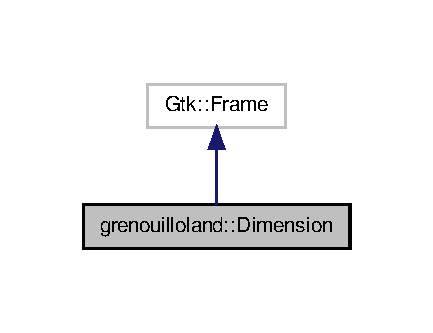
\includegraphics[width=208pt]{classgrenouilloland_1_1Dimension__inherit__graph}
\end{center}
\end{figure}


Graphe de collaboration de grenouilloland\-:\-:Dimension\-:
\nopagebreak
\begin{figure}[H]
\begin{center}
\leavevmode
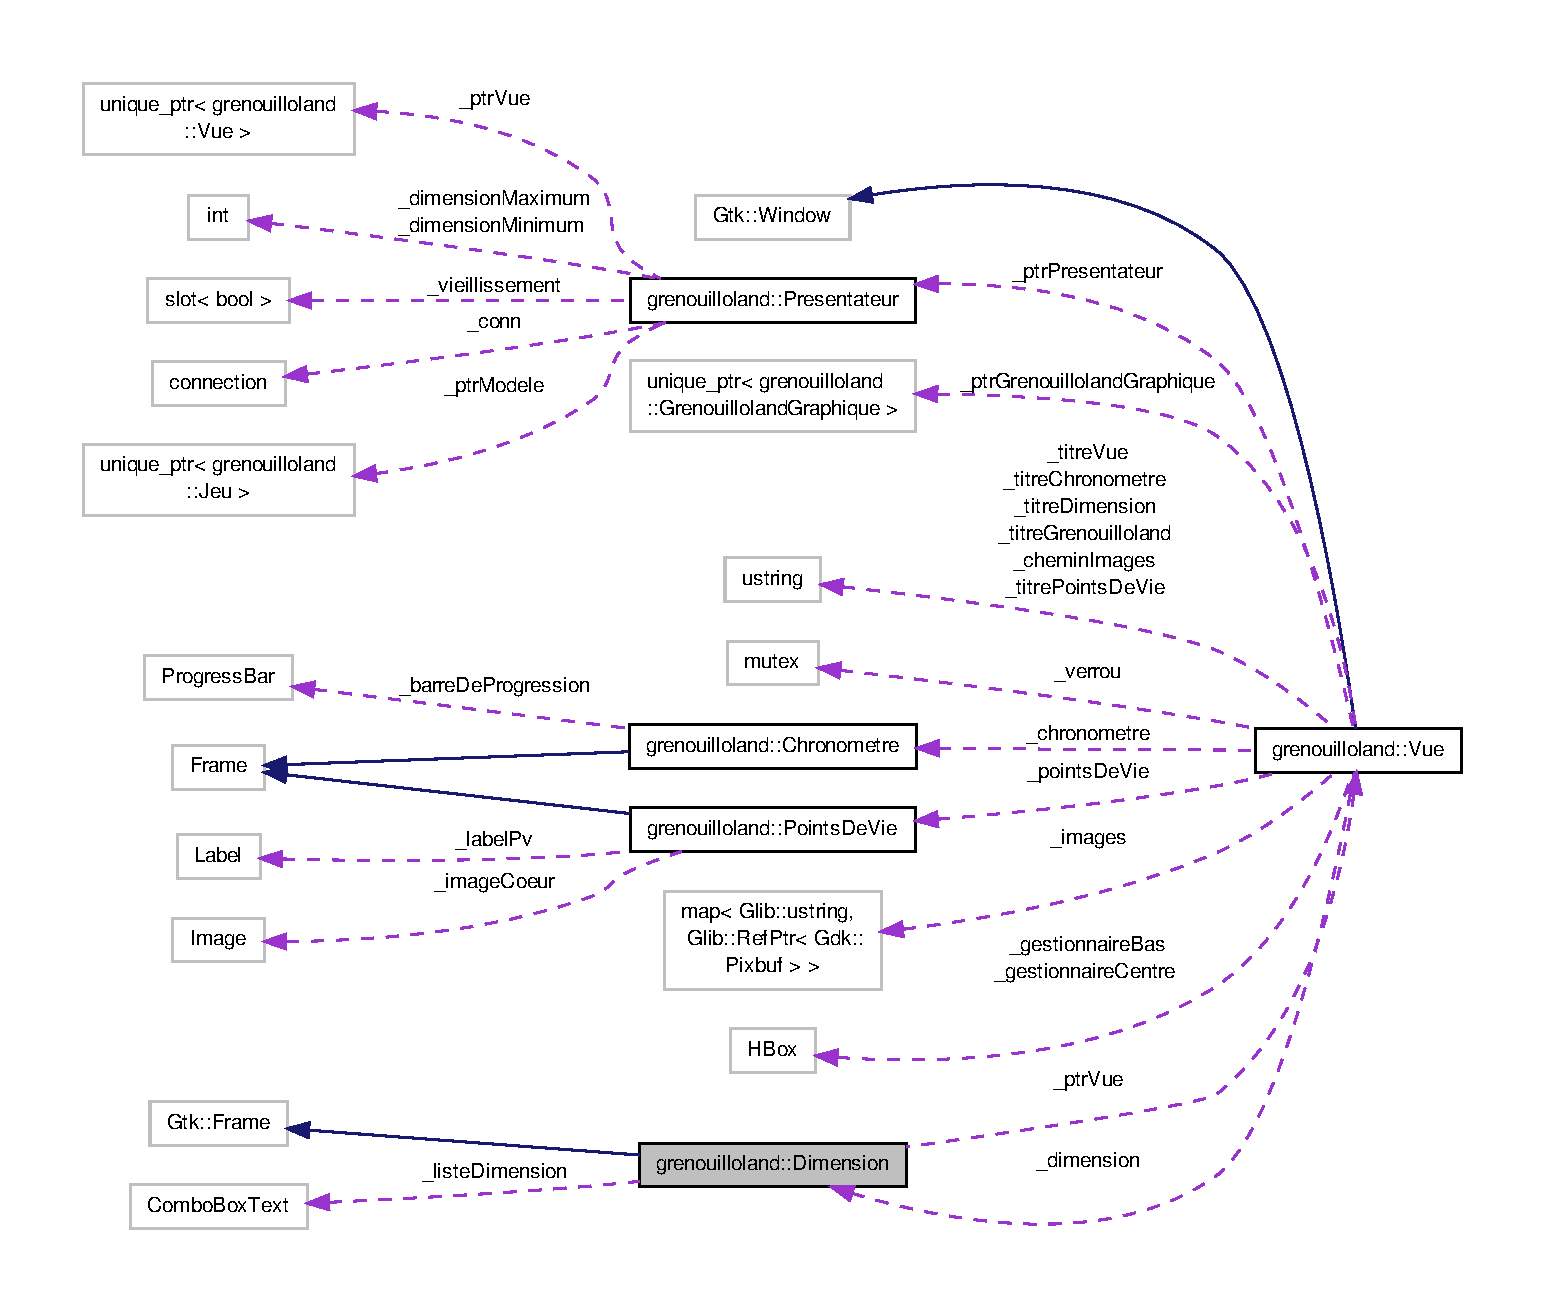
\includegraphics[width=350pt]{classgrenouilloland_1_1Dimension__coll__graph}
\end{center}
\end{figure}
\subsection*{Fonctions membres publiques}
\begin{DoxyCompactItemize}
\item 
\hyperlink{classgrenouilloland_1_1Dimension_ac90aede2a2de82759014e3ff8f4eed6f}{Dimension} (const Glib\-::ustring \&titre, \hyperlink{classgrenouilloland_1_1Vue}{Vue} \&vue)
\item 
const \hyperlink{classgrenouilloland_1_1Vue}{Vue} \& \hyperlink{classgrenouilloland_1_1Dimension_a7daf1ff22e3c4d1085c35ff7b333760b}{lire\-Vue} () const 
\item 
int \hyperlink{classgrenouilloland_1_1Dimension_a3d82e721e31be8656926fc157f38ea1c}{valeur} () const 
\end{DoxyCompactItemize}
\subsection*{Fonctions membres protégées}
\begin{DoxyCompactItemize}
\item 
void \hyperlink{classgrenouilloland_1_1Dimension_a7415e793d4ea98afe30864e81e00e48b}{cb\-Changement\-De\-Valeur} ()
\end{DoxyCompactItemize}
\subsection*{Attributs protégés}
\begin{DoxyCompactItemize}
\item 
\hyperlink{classgrenouilloland_1_1Vue}{Vue} $\ast$const \hyperlink{classgrenouilloland_1_1Dimension_a5b66fbce9d7f6eed85d39f90bb71d7c7}{\-\_\-ptr\-Vue}
\item 
Gtk\-::\-Combo\-Box\-Text \hyperlink{classgrenouilloland_1_1Dimension_aea2f6714737f26588395db30cb0385bd}{\-\_\-liste\-Dimension}
\end{DoxyCompactItemize}


\subsection{Description détaillée}
Controleur de la dimension du \hyperlink{classgrenouilloland_1_1Jeu}{Jeu}. 

\begin{DoxyAuthor}{Auteur}
Yann Dauxais 

Alexandre Beudin 
\end{DoxyAuthor}
\begin{DoxyDate}{Date}
6.\-1.\-2013
\end{DoxyDate}
Declaration de la classe \hyperlink{classgrenouilloland_1_1Dimension}{Dimension} representant le controleur de dimension du \hyperlink{classgrenouilloland_1_1Jeu}{Jeu}. Le Widget utilisé est un menu déroulant.

\begin{DoxyNote}{Note}
une instance de cette classe ne peut etre dupliquee.

chaque instance de cette classe est son propre listener. 
\end{DoxyNote}


\subsection{Documentation des constructeurs et destructeur}
\hypertarget{classgrenouilloland_1_1Dimension_ac90aede2a2de82759014e3ff8f4eed6f}{\index{grenouilloland\-::\-Dimension@{grenouilloland\-::\-Dimension}!Dimension@{Dimension}}
\index{Dimension@{Dimension}!grenouilloland::Dimension@{grenouilloland\-::\-Dimension}}
\subsubsection[{Dimension}]{\setlength{\rightskip}{0pt plus 5cm}Dimension\-::\-Dimension (
\begin{DoxyParamCaption}
\item[{const Glib\-::ustring \&}]{titre, }
\item[{{\bf Vue} \&}]{vue}
\end{DoxyParamCaption}
)}}\label{classgrenouilloland_1_1Dimension_ac90aede2a2de82759014e3ff8f4eed6f}
Constructeur logique.


\begin{DoxyParams}[1]{Paramètres}
\mbox{\tt in}  & {\em titre} & -\/ le titre du contour. \\
\hline
\mbox{\tt in,out}  & {\em vue} & -\/ la valeur de \hyperlink{classgrenouilloland_1_1Dimension_a5b66fbce9d7f6eed85d39f90bb71d7c7}{\-\_\-ptr\-Vue}. \\
\hline
\end{DoxyParams}


\subsection{Documentation des fonctions membres}
\hypertarget{classgrenouilloland_1_1Dimension_a7415e793d4ea98afe30864e81e00e48b}{\index{grenouilloland\-::\-Dimension@{grenouilloland\-::\-Dimension}!cb\-Changement\-De\-Valeur@{cb\-Changement\-De\-Valeur}}
\index{cb\-Changement\-De\-Valeur@{cb\-Changement\-De\-Valeur}!grenouilloland::Dimension@{grenouilloland\-::\-Dimension}}
\subsubsection[{cb\-Changement\-De\-Valeur}]{\setlength{\rightskip}{0pt plus 5cm}void Dimension\-::cb\-Changement\-De\-Valeur (
\begin{DoxyParamCaption}
{}
\end{DoxyParamCaption}
)\hspace{0.3cm}{\ttfamily [protected]}}}\label{classgrenouilloland_1_1Dimension_a7415e793d4ea98afe30864e81e00e48b}
Callback associe au changement de valeur. \hypertarget{classgrenouilloland_1_1Dimension_a7daf1ff22e3c4d1085c35ff7b333760b}{\index{grenouilloland\-::\-Dimension@{grenouilloland\-::\-Dimension}!lire\-Vue@{lire\-Vue}}
\index{lire\-Vue@{lire\-Vue}!grenouilloland::Dimension@{grenouilloland\-::\-Dimension}}
\subsubsection[{lire\-Vue}]{\setlength{\rightskip}{0pt plus 5cm}const {\bf Vue} \& Dimension\-::lire\-Vue (
\begin{DoxyParamCaption}
{}
\end{DoxyParamCaption}
) const}}\label{classgrenouilloland_1_1Dimension_a7daf1ff22e3c4d1085c35ff7b333760b}
Accesseur.

\begin{DoxyReturn}{Renvoie}
la valeur de \hyperlink{classgrenouilloland_1_1Dimension_a5b66fbce9d7f6eed85d39f90bb71d7c7}{\-\_\-ptr\-Vue}. 
\end{DoxyReturn}
\hypertarget{classgrenouilloland_1_1Dimension_a3d82e721e31be8656926fc157f38ea1c}{\index{grenouilloland\-::\-Dimension@{grenouilloland\-::\-Dimension}!valeur@{valeur}}
\index{valeur@{valeur}!grenouilloland::Dimension@{grenouilloland\-::\-Dimension}}
\subsubsection[{valeur}]{\setlength{\rightskip}{0pt plus 5cm}int Dimension\-::valeur (
\begin{DoxyParamCaption}
{}
\end{DoxyParamCaption}
) const}}\label{classgrenouilloland_1_1Dimension_a3d82e721e31be8656926fc157f38ea1c}
Retourne la dimension actuelle.

\begin{DoxyReturn}{Renvoie}
la dimension actuelle. 
\end{DoxyReturn}


\subsection{Documentation des données membres}
\hypertarget{classgrenouilloland_1_1Dimension_aea2f6714737f26588395db30cb0385bd}{\index{grenouilloland\-::\-Dimension@{grenouilloland\-::\-Dimension}!\-\_\-liste\-Dimension@{\-\_\-liste\-Dimension}}
\index{\-\_\-liste\-Dimension@{\-\_\-liste\-Dimension}!grenouilloland::Dimension@{grenouilloland\-::\-Dimension}}
\subsubsection[{\-\_\-liste\-Dimension}]{\setlength{\rightskip}{0pt plus 5cm}Gtk\-::\-Combo\-Box\-Text grenouilloland\-::\-Dimension\-::\-\_\-liste\-Dimension\hspace{0.3cm}{\ttfamily [protected]}}}\label{classgrenouilloland_1_1Dimension_aea2f6714737f26588395db30cb0385bd}
Menu déroulant. \hypertarget{classgrenouilloland_1_1Dimension_a5b66fbce9d7f6eed85d39f90bb71d7c7}{\index{grenouilloland\-::\-Dimension@{grenouilloland\-::\-Dimension}!\-\_\-ptr\-Vue@{\-\_\-ptr\-Vue}}
\index{\-\_\-ptr\-Vue@{\-\_\-ptr\-Vue}!grenouilloland::Dimension@{grenouilloland\-::\-Dimension}}
\subsubsection[{\-\_\-ptr\-Vue}]{\setlength{\rightskip}{0pt plus 5cm}{\bf Vue}$\ast$ const grenouilloland\-::\-Dimension\-::\-\_\-ptr\-Vue\hspace{0.3cm}{\ttfamily [protected]}}}\label{classgrenouilloland_1_1Dimension_a5b66fbce9d7f6eed85d39f90bb71d7c7}
Unique vue proprietaire de ce controleur. 

La documentation de cette classe a été générée à partir des fichiers suivants \-:\begin{DoxyCompactItemize}
\item 
src/vue/include/Dimension.\-hh\item 
src/vue/Dimension.\-cpp\end{DoxyCompactItemize}

\hypertarget{classgrenouilloland_1_1Eau}{\section{Référence de la classe grenouilloland\-:\-:Eau}
\label{classgrenouilloland_1_1Eau}\index{grenouilloland\-::\-Eau@{grenouilloland\-::\-Eau}}
}


\hyperlink{classgrenouilloland_1_1Case}{Case} du \hyperlink{classgrenouilloland_1_1Jeu}{Jeu} Grenouilloland.  




{\ttfamily \#include $<$Eau.\-hh$>$}



Graphe d'héritage de grenouilloland\-:\-:Eau\-:
\nopagebreak
\begin{figure}[H]
\begin{center}
\leavevmode
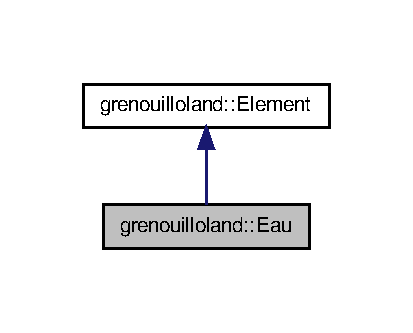
\includegraphics[width=198pt]{classgrenouilloland_1_1Eau__inherit__graph}
\end{center}
\end{figure}


Graphe de collaboration de grenouilloland\-:\-:Eau\-:
\nopagebreak
\begin{figure}[H]
\begin{center}
\leavevmode
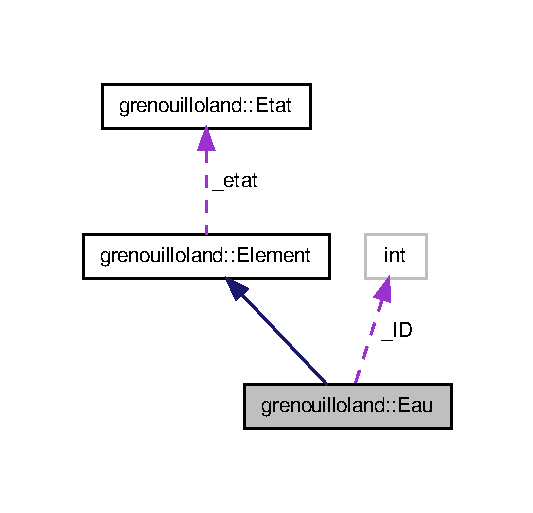
\includegraphics[width=256pt]{classgrenouilloland_1_1Eau__coll__graph}
\end{center}
\end{figure}
\subsection*{Fonctions membres publiques}
\begin{DoxyCompactItemize}
\item 
\hyperlink{classgrenouilloland_1_1Eau_aeebcde96afd822158f1c5f5daee8b67b}{Eau} ()
\item 
\hyperlink{classgrenouilloland_1_1Eau_aa7620d18dc4dcc19ebcfb2cd44cf788d}{$\sim$\-Eau} ()
\item 
const int \& \hyperlink{classgrenouilloland_1_1Eau_a649c33d717a7bec06683a18cbd13bd52}{lire\-Id} () const 
\item 
bool \hyperlink{classgrenouilloland_1_1Eau_afddd34ea4f2babcfe78b1be9dfd2f7af}{is\-Eau} () const 
\end{DoxyCompactItemize}
\subsection*{Attributs publics statiques}
\begin{DoxyCompactItemize}
\item 
static const int \hyperlink{classgrenouilloland_1_1Eau_af354ad9fa95f55695d0463a8cc2cbcb0}{\-\_\-\-I\-D}
\end{DoxyCompactItemize}
\subsection*{Additional Inherited Members}


\subsection{Description détaillée}
\hyperlink{classgrenouilloland_1_1Case}{Case} du \hyperlink{classgrenouilloland_1_1Jeu}{Jeu} Grenouilloland. 

\begin{DoxyAuthor}{Auteur}
Beudin.\-Alexandre Dauxais.\-Yann 
\end{DoxyAuthor}
\begin{DoxyDate}{Date}
05.\-01.\-2012
\end{DoxyDate}
Declaration de la classe \hyperlink{classgrenouilloland_1_1Eau}{Eau} réprésentant l'élément d'eau dans le jeu Grenouilloland. 

\subsection{Documentation des constructeurs et destructeur}
\hypertarget{classgrenouilloland_1_1Eau_aeebcde96afd822158f1c5f5daee8b67b}{\index{grenouilloland\-::\-Eau@{grenouilloland\-::\-Eau}!Eau@{Eau}}
\index{Eau@{Eau}!grenouilloland::Eau@{grenouilloland\-::\-Eau}}
\subsubsection[{Eau}]{\setlength{\rightskip}{0pt plus 5cm}Eau\-::\-Eau (
\begin{DoxyParamCaption}
{}
\end{DoxyParamCaption}
)}}\label{classgrenouilloland_1_1Eau_aeebcde96afd822158f1c5f5daee8b67b}
Constructeur par défaut instanciant de l'eau. \hypertarget{classgrenouilloland_1_1Eau_aa7620d18dc4dcc19ebcfb2cd44cf788d}{\index{grenouilloland\-::\-Eau@{grenouilloland\-::\-Eau}!$\sim$\-Eau@{$\sim$\-Eau}}
\index{$\sim$\-Eau@{$\sim$\-Eau}!grenouilloland::Eau@{grenouilloland\-::\-Eau}}
\subsubsection[{$\sim$\-Eau}]{\setlength{\rightskip}{0pt plus 5cm}Eau\-::$\sim$\-Eau (
\begin{DoxyParamCaption}
{}
\end{DoxyParamCaption}
)}}\label{classgrenouilloland_1_1Eau_aa7620d18dc4dcc19ebcfb2cd44cf788d}
Destructeur d'un élément d'eau. 

\subsection{Documentation des fonctions membres}
\hypertarget{classgrenouilloland_1_1Eau_afddd34ea4f2babcfe78b1be9dfd2f7af}{\index{grenouilloland\-::\-Eau@{grenouilloland\-::\-Eau}!is\-Eau@{is\-Eau}}
\index{is\-Eau@{is\-Eau}!grenouilloland::Eau@{grenouilloland\-::\-Eau}}
\subsubsection[{is\-Eau}]{\setlength{\rightskip}{0pt plus 5cm}bool Eau\-::is\-Eau (
\begin{DoxyParamCaption}
{}
\end{DoxyParamCaption}
) const\hspace{0.3cm}{\ttfamily [virtual]}}}\label{classgrenouilloland_1_1Eau_afddd34ea4f2babcfe78b1be9dfd2f7af}
Méthode permettant de détecter si l'élément est de l'eau.

\begin{DoxyReturn}{Renvoie}
true. 
\end{DoxyReturn}


Réimplémentée à partir de \hyperlink{classgrenouilloland_1_1Element_adf2a739bbd6b529dc387cb95cb925f53}{grenouilloland\-::\-Element}.

\hypertarget{classgrenouilloland_1_1Eau_a649c33d717a7bec06683a18cbd13bd52}{\index{grenouilloland\-::\-Eau@{grenouilloland\-::\-Eau}!lire\-Id@{lire\-Id}}
\index{lire\-Id@{lire\-Id}!grenouilloland::Eau@{grenouilloland\-::\-Eau}}
\subsubsection[{lire\-Id}]{\setlength{\rightskip}{0pt plus 5cm}const int \& Eau\-::lire\-Id (
\begin{DoxyParamCaption}
{}
\end{DoxyParamCaption}
) const\hspace{0.3cm}{\ttfamily [virtual]}}}\label{classgrenouilloland_1_1Eau_a649c33d717a7bec06683a18cbd13bd52}
Accesseur de l'\-\_\-\-I\-D identifiant l'eau.

\begin{DoxyReturn}{Renvoie}
la valeur de \hyperlink{classgrenouilloland_1_1Eau_af354ad9fa95f55695d0463a8cc2cbcb0}{\-\_\-\-I\-D}.
\end{DoxyReturn}
\begin{DoxyNote}{Note}
L'\-\_\-\-I\-D est const et public mais cet accesseur est nécessaire car il est lu dans la vue sur un objet de type \hyperlink{classgrenouilloland_1_1Element}{Element} et un \hyperlink{classgrenouilloland_1_1Element}{Element} n'a pas d'attribut \-\_\-\-I\-D. 
\end{DoxyNote}


Implémente \hyperlink{classgrenouilloland_1_1Element_aa05b1a2f2e0e8eb0e5ebf942b8934388}{grenouilloland\-::\-Element}.



\subsection{Documentation des données membres}
\hypertarget{classgrenouilloland_1_1Eau_af354ad9fa95f55695d0463a8cc2cbcb0}{\index{grenouilloland\-::\-Eau@{grenouilloland\-::\-Eau}!\-\_\-\-I\-D@{\-\_\-\-I\-D}}
\index{\-\_\-\-I\-D@{\-\_\-\-I\-D}!grenouilloland::Eau@{grenouilloland\-::\-Eau}}
\subsubsection[{\-\_\-\-I\-D}]{\setlength{\rightskip}{0pt plus 5cm}const int Eau\-::\-\_\-\-I\-D\hspace{0.3cm}{\ttfamily [static]}}}\label{classgrenouilloland_1_1Eau_af354ad9fa95f55695d0463a8cc2cbcb0}
I\-D identifiant l'eau pour associer une image. 

La documentation de cette classe a été générée à partir des fichiers suivants \-:\begin{DoxyCompactItemize}
\item 
src/modele/include/Eau.\-hh\item 
src/modele/Eau.\-cpp\end{DoxyCompactItemize}

\hypertarget{classgrenouilloland_1_1Element}{\section{Référence de la classe grenouilloland\-:\-:Element}
\label{classgrenouilloland_1_1Element}\index{grenouilloland\-::\-Element@{grenouilloland\-::\-Element}}
}


\hyperlink{classgrenouilloland_1_1Element}{Element} du \hyperlink{classgrenouilloland_1_1Jeu}{Jeu} Grenouilloland.  




{\ttfamily \#include $<$Element.\-hh$>$}



Graphe d'héritage de grenouilloland\-:\-:Element\-:
\nopagebreak
\begin{figure}[H]
\begin{center}
\leavevmode
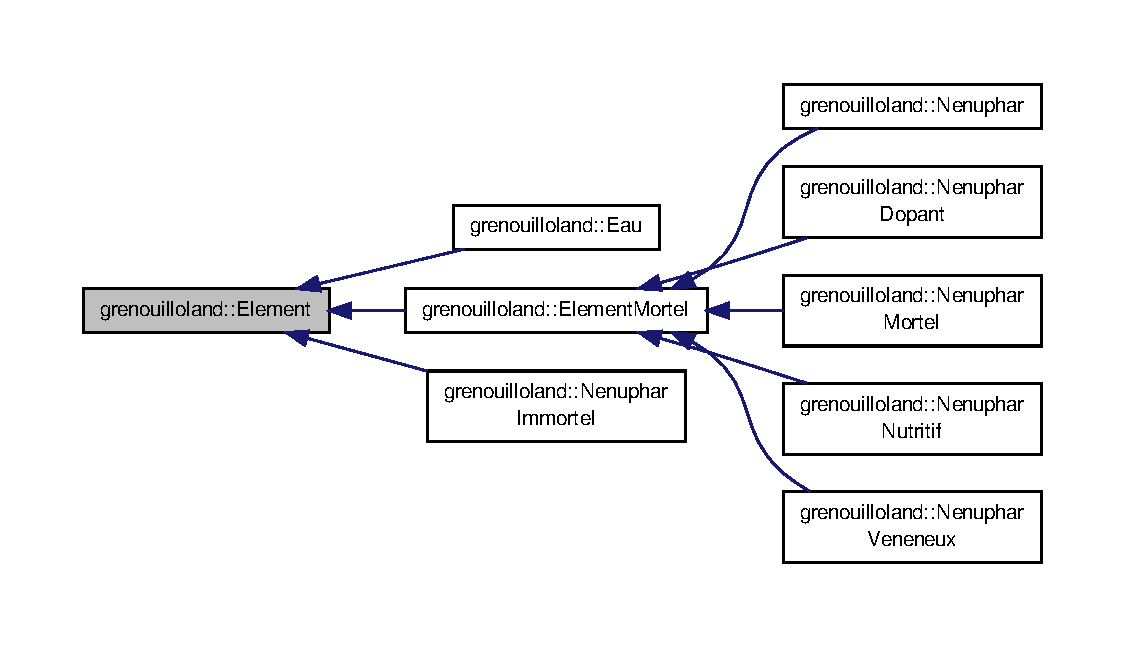
\includegraphics[width=350pt]{classgrenouilloland_1_1Element__inherit__graph}
\end{center}
\end{figure}


Graphe de collaboration de grenouilloland\-:\-:Element\-:
\nopagebreak
\begin{figure}[H]
\begin{center}
\leavevmode
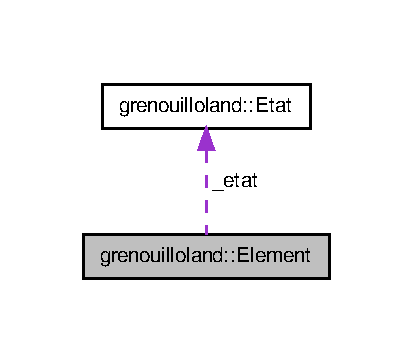
\includegraphics[width=198pt]{classgrenouilloland_1_1Element__coll__graph}
\end{center}
\end{figure}
\subsection*{Classes}
\begin{DoxyCompactItemize}
\item 
class \hyperlink{classgrenouilloland_1_1Element_1_1Mandataire}{Mandataire}
\begin{DoxyCompactList}\small\item\em \hyperlink{classgrenouilloland_1_1Element_1_1Mandataire}{Mandataire} de la classe \hyperlink{classgrenouilloland_1_1Element}{Element} du \hyperlink{classgrenouilloland_1_1Jeu}{Jeu} Grenouilloland. \end{DoxyCompactList}\end{DoxyCompactItemize}
\subsection*{Fonctions membres publiques}
\begin{DoxyCompactItemize}
\item 
virtual \hyperlink{classgrenouilloland_1_1Element_aa66f20df4bbbd9c2253f80e612204f18}{$\sim$\-Element} ()=0
\item 
virtual const int \& \hyperlink{classgrenouilloland_1_1Element_aa05b1a2f2e0e8eb0e5ebf942b8934388}{lire\-Id} () const =0
\item 
virtual bool \hyperlink{classgrenouilloland_1_1Element_adf2a739bbd6b529dc387cb95cb925f53}{is\-Eau} () const 
\item 
const \hyperlink{classgrenouilloland_1_1Etat}{Etat} \& \hyperlink{classgrenouilloland_1_1Element_a2391eb9fde2b7d5afd8588f9141d0a35}{lire\-Etat} () const 
\end{DoxyCompactItemize}
\subsection*{Fonctions membres protégées}
\begin{DoxyCompactItemize}
\item 
\hyperlink{classgrenouilloland_1_1Element_a6177b43ce377505948db0db58316fa0f}{Element} (const \hyperlink{classgrenouilloland_1_1StrategieAbstraite}{Strategie\-Abstraite} \&strategie)
\end{DoxyCompactItemize}
\subsection*{Attributs protégés}
\begin{DoxyCompactItemize}
\item 
\hyperlink{classgrenouilloland_1_1Etat}{Etat} \hyperlink{classgrenouilloland_1_1Element_a6c404d7c7e11b3add7b2cc899c4a3685}{\-\_\-etat}
\end{DoxyCompactItemize}


\subsection{Description détaillée}
\hyperlink{classgrenouilloland_1_1Element}{Element} du \hyperlink{classgrenouilloland_1_1Jeu}{Jeu} Grenouilloland. 

\begin{DoxyAuthor}{Auteur}
Beudin.\-Alexandre Dauxais.\-Yann 
\end{DoxyAuthor}
\begin{DoxyDate}{Date}
05.\-01.\-2012
\end{DoxyDate}
Declaration de la classe abstraite \hyperlink{classgrenouilloland_1_1Element}{Element} réprésentant la structure d'un élément du jeu Grenouilloland. 

\subsection{Documentation des constructeurs et destructeur}
\hypertarget{classgrenouilloland_1_1Element_aa66f20df4bbbd9c2253f80e612204f18}{\index{grenouilloland\-::\-Element@{grenouilloland\-::\-Element}!$\sim$\-Element@{$\sim$\-Element}}
\index{$\sim$\-Element@{$\sim$\-Element}!grenouilloland::Element@{grenouilloland\-::\-Element}}
\subsubsection[{$\sim$\-Element}]{\setlength{\rightskip}{0pt plus 5cm}Element\-::$\sim$\-Element (
\begin{DoxyParamCaption}
{}
\end{DoxyParamCaption}
)\hspace{0.3cm}{\ttfamily [pure virtual]}}}\label{classgrenouilloland_1_1Element_aa66f20df4bbbd9c2253f80e612204f18}
Destructeur de l'élément. \hypertarget{classgrenouilloland_1_1Element_a6177b43ce377505948db0db58316fa0f}{\index{grenouilloland\-::\-Element@{grenouilloland\-::\-Element}!Element@{Element}}
\index{Element@{Element}!grenouilloland::Element@{grenouilloland\-::\-Element}}
\subsubsection[{Element}]{\setlength{\rightskip}{0pt plus 5cm}Element\-::\-Element (
\begin{DoxyParamCaption}
\item[{const {\bf Strategie\-Abstraite} \&}]{strategie}
\end{DoxyParamCaption}
)\hspace{0.3cm}{\ttfamily [protected]}}}\label{classgrenouilloland_1_1Element_a6177b43ce377505948db0db58316fa0f}
Constructeur logique instanciant un élément.


\begin{DoxyParams}[1]{Paramètres}
\mbox{\tt in}  & {\em strategie} & -\/ stratégie appliqué par l'élément. \\
\hline
\end{DoxyParams}


\subsection{Documentation des fonctions membres}
\hypertarget{classgrenouilloland_1_1Element_adf2a739bbd6b529dc387cb95cb925f53}{\index{grenouilloland\-::\-Element@{grenouilloland\-::\-Element}!is\-Eau@{is\-Eau}}
\index{is\-Eau@{is\-Eau}!grenouilloland::Element@{grenouilloland\-::\-Element}}
\subsubsection[{is\-Eau}]{\setlength{\rightskip}{0pt plus 5cm}bool Element\-::is\-Eau (
\begin{DoxyParamCaption}
{}
\end{DoxyParamCaption}
) const\hspace{0.3cm}{\ttfamily [virtual]}}}\label{classgrenouilloland_1_1Element_adf2a739bbd6b529dc387cb95cb925f53}
Méthode permettant de détecter si l'élément est de l'eau.

return false. 

Réimplémentée dans \hyperlink{classgrenouilloland_1_1Eau_afddd34ea4f2babcfe78b1be9dfd2f7af}{grenouilloland\-::\-Eau}.

\hypertarget{classgrenouilloland_1_1Element_a2391eb9fde2b7d5afd8588f9141d0a35}{\index{grenouilloland\-::\-Element@{grenouilloland\-::\-Element}!lire\-Etat@{lire\-Etat}}
\index{lire\-Etat@{lire\-Etat}!grenouilloland::Element@{grenouilloland\-::\-Element}}
\subsubsection[{lire\-Etat}]{\setlength{\rightskip}{0pt plus 5cm}const {\bf Etat} \& Element\-::lire\-Etat (
\begin{DoxyParamCaption}
{}
\end{DoxyParamCaption}
) const}}\label{classgrenouilloland_1_1Element_a2391eb9fde2b7d5afd8588f9141d0a35}
Accesseur de l'état de l'élément.

\begin{DoxyReturn}{Renvoie}
valeur de \hyperlink{classgrenouilloland_1_1Element_a6c404d7c7e11b3add7b2cc899c4a3685}{\-\_\-etat}. 
\end{DoxyReturn}
\hypertarget{classgrenouilloland_1_1Element_aa05b1a2f2e0e8eb0e5ebf942b8934388}{\index{grenouilloland\-::\-Element@{grenouilloland\-::\-Element}!lire\-Id@{lire\-Id}}
\index{lire\-Id@{lire\-Id}!grenouilloland::Element@{grenouilloland\-::\-Element}}
\subsubsection[{lire\-Id}]{\setlength{\rightskip}{0pt plus 5cm}virtual const int\& grenouilloland\-::\-Element\-::lire\-Id (
\begin{DoxyParamCaption}
{}
\end{DoxyParamCaption}
) const\hspace{0.3cm}{\ttfamily [pure virtual]}}}\label{classgrenouilloland_1_1Element_aa05b1a2f2e0e8eb0e5ebf942b8934388}
Accesseur de l'I\-D identifiant le type de l'élément.

\begin{DoxyReturn}{Renvoie}
valeur de l'I\-D. 
\end{DoxyReturn}


Implémenté dans \hyperlink{classgrenouilloland_1_1Eau_a649c33d717a7bec06683a18cbd13bd52}{grenouilloland\-::\-Eau}, \hyperlink{classgrenouilloland_1_1Nenuphar_a3a77c3463dd389cf0eee275ee96a7939}{grenouilloland\-::\-Nenuphar}, \hyperlink{classgrenouilloland_1_1NenupharDopant_a45374c5e71552f943b8a9729892d5f02}{grenouilloland\-::\-Nenuphar\-Dopant}, \hyperlink{classgrenouilloland_1_1NenupharImmortel_a6fadef66c4d46dea30e0b5ba933ff1d6}{grenouilloland\-::\-Nenuphar\-Immortel}, \hyperlink{classgrenouilloland_1_1NenupharMortel_aac1c7add92c76c06a2848fe264a59bdd}{grenouilloland\-::\-Nenuphar\-Mortel}, \hyperlink{classgrenouilloland_1_1NenupharNutritif_ac27d0cfbf8e2f4ee647031983a5fc1f4}{grenouilloland\-::\-Nenuphar\-Nutritif}, et \hyperlink{classgrenouilloland_1_1NenupharVeneneux_afbf5c6a0b2f88d65027a6582dca402d1}{grenouilloland\-::\-Nenuphar\-Veneneux}.



\subsection{Documentation des données membres}
\hypertarget{classgrenouilloland_1_1Element_a6c404d7c7e11b3add7b2cc899c4a3685}{\index{grenouilloland\-::\-Element@{grenouilloland\-::\-Element}!\-\_\-etat@{\-\_\-etat}}
\index{\-\_\-etat@{\-\_\-etat}!grenouilloland::Element@{grenouilloland\-::\-Element}}
\subsubsection[{\-\_\-etat}]{\setlength{\rightskip}{0pt plus 5cm}{\bf Etat} grenouilloland\-::\-Element\-::\-\_\-etat\hspace{0.3cm}{\ttfamily [protected]}}}\label{classgrenouilloland_1_1Element_a6c404d7c7e11b3add7b2cc899c4a3685}
\hyperlink{classgrenouilloland_1_1Etat}{Etat} de l'élément. 

La documentation de cette classe a été générée à partir des fichiers suivants \-:\begin{DoxyCompactItemize}
\item 
src/modele/include/Element.\-hh\item 
src/modele/Element.\-cpp\end{DoxyCompactItemize}

\hypertarget{classgrenouilloland_1_1ElementMortel}{\section{Référence de la classe grenouilloland\-:\-:Element\-Mortel}
\label{classgrenouilloland_1_1ElementMortel}\index{grenouilloland\-::\-Element\-Mortel@{grenouilloland\-::\-Element\-Mortel}}
}


\hyperlink{classgrenouilloland_1_1ElementMortel}{Element\-Mortel} du \hyperlink{classgrenouilloland_1_1Jeu}{Jeu} Grenouilloland.  




{\ttfamily \#include $<$Element\-Mortel.\-hh$>$}



Graphe d'héritage de grenouilloland\-:\-:Element\-Mortel\-:
\nopagebreak
\begin{figure}[H]
\begin{center}
\leavevmode
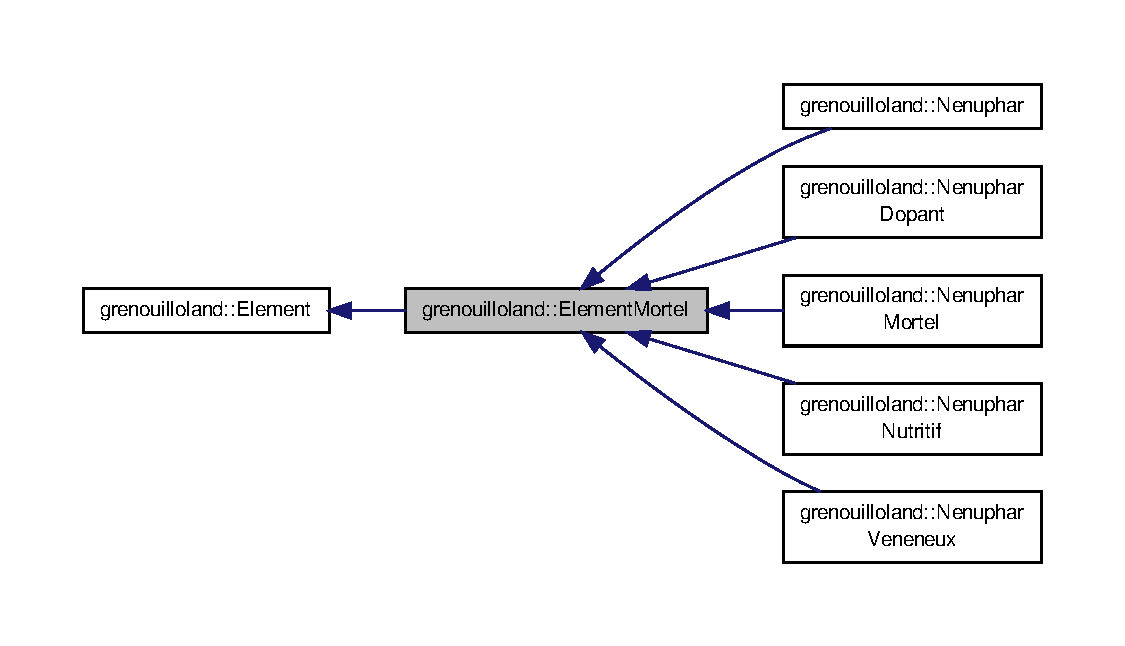
\includegraphics[width=350pt]{classgrenouilloland_1_1ElementMortel__inherit__graph}
\end{center}
\end{figure}


Graphe de collaboration de grenouilloland\-:\-:Element\-Mortel\-:
\nopagebreak
\begin{figure}[H]
\begin{center}
\leavevmode
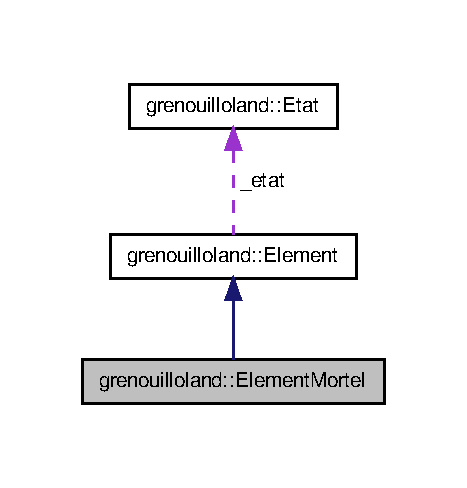
\includegraphics[width=224pt]{classgrenouilloland_1_1ElementMortel__coll__graph}
\end{center}
\end{figure}
\subsection*{Fonctions membres publiques}
\begin{DoxyCompactItemize}
\item 
virtual \hyperlink{classgrenouilloland_1_1ElementMortel_af3b98e89d6adca1cb01d148d9fb4da02}{$\sim$\-Element\-Mortel} ()=0
\end{DoxyCompactItemize}
\subsection*{Fonctions membres protégées}
\begin{DoxyCompactItemize}
\item 
\hyperlink{classgrenouilloland_1_1ElementMortel_afcc0659282b7c248c5546f4169a5165f}{Element\-Mortel} (const \hyperlink{classgrenouilloland_1_1StrategieAbstraite}{Strategie\-Abstraite} \&strategie)
\item 
\hyperlink{classgrenouilloland_1_1Etat}{Etat} \hyperlink{classgrenouilloland_1_1ElementMortel_a300a32cce88feb6a2bfc92c1165f9c61}{vieillir} ()
\end{DoxyCompactItemize}
\subsection*{Additional Inherited Members}


\subsection{Description détaillée}
\hyperlink{classgrenouilloland_1_1ElementMortel}{Element\-Mortel} du \hyperlink{classgrenouilloland_1_1Jeu}{Jeu} Grenouilloland. 

\begin{DoxyAuthor}{Auteur}
Beudin.\-Alexandre Dauxais.\-Yann 
\end{DoxyAuthor}
\begin{DoxyDate}{Date}
05.\-01.\-2012
\end{DoxyDate}
Declaration de la classe abstraite \hyperlink{classgrenouilloland_1_1ElementMortel}{Element\-Mortel} réprésentant la structure d'un élément ayant plusieurs états de vieillissement du jeu Grenouilloland. 

\subsection{Documentation des constructeurs et destructeur}
\hypertarget{classgrenouilloland_1_1ElementMortel_af3b98e89d6adca1cb01d148d9fb4da02}{\index{grenouilloland\-::\-Element\-Mortel@{grenouilloland\-::\-Element\-Mortel}!$\sim$\-Element\-Mortel@{$\sim$\-Element\-Mortel}}
\index{$\sim$\-Element\-Mortel@{$\sim$\-Element\-Mortel}!grenouilloland::ElementMortel@{grenouilloland\-::\-Element\-Mortel}}
\subsubsection[{$\sim$\-Element\-Mortel}]{\setlength{\rightskip}{0pt plus 5cm}Element\-Mortel\-::$\sim$\-Element\-Mortel (
\begin{DoxyParamCaption}
{}
\end{DoxyParamCaption}
)\hspace{0.3cm}{\ttfamily [pure virtual]}}}\label{classgrenouilloland_1_1ElementMortel_af3b98e89d6adca1cb01d148d9fb4da02}
Destructeur d'un élément mortel. \hypertarget{classgrenouilloland_1_1ElementMortel_afcc0659282b7c248c5546f4169a5165f}{\index{grenouilloland\-::\-Element\-Mortel@{grenouilloland\-::\-Element\-Mortel}!Element\-Mortel@{Element\-Mortel}}
\index{Element\-Mortel@{Element\-Mortel}!grenouilloland::ElementMortel@{grenouilloland\-::\-Element\-Mortel}}
\subsubsection[{Element\-Mortel}]{\setlength{\rightskip}{0pt plus 5cm}Element\-Mortel\-::\-Element\-Mortel (
\begin{DoxyParamCaption}
\item[{const {\bf Strategie\-Abstraite} \&}]{strategie}
\end{DoxyParamCaption}
)\hspace{0.3cm}{\ttfamily [protected]}}}\label{classgrenouilloland_1_1ElementMortel_afcc0659282b7c248c5546f4169a5165f}
Constructeur logique d'un élément mortel.


\begin{DoxyParams}[1]{Paramètres}
\mbox{\tt in}  & {\em strategie} & -\/ stratégie de l'élément mortel. \\
\hline
\end{DoxyParams}


\subsection{Documentation des fonctions membres}
\hypertarget{classgrenouilloland_1_1ElementMortel_a300a32cce88feb6a2bfc92c1165f9c61}{\index{grenouilloland\-::\-Element\-Mortel@{grenouilloland\-::\-Element\-Mortel}!vieillir@{vieillir}}
\index{vieillir@{vieillir}!grenouilloland::ElementMortel@{grenouilloland\-::\-Element\-Mortel}}
\subsubsection[{vieillir}]{\setlength{\rightskip}{0pt plus 5cm}{\bf Etat} Element\-Mortel\-::vieillir (
\begin{DoxyParamCaption}
{}
\end{DoxyParamCaption}
)\hspace{0.3cm}{\ttfamily [protected]}, {\ttfamily [virtual]}}}\label{classgrenouilloland_1_1ElementMortel_a300a32cce88feb6a2bfc92c1165f9c61}
Vieillissement de l'élément mortel.

\begin{DoxyReturn}{Renvoie}
l'état de l'élément mortel. 
\end{DoxyReturn}


Réimplémentée à partir de \hyperlink{classgrenouilloland_1_1Element}{grenouilloland\-::\-Element}.



La documentation de cette classe a été générée à partir des fichiers suivants \-:\begin{DoxyCompactItemize}
\item 
src/modele/include/Element\-Mortel.\-hh\item 
src/modele/Element\-Mortel.\-cpp\end{DoxyCompactItemize}

\hypertarget{classgrenouilloland_1_1Etat}{\section{Référence de la classe grenouilloland\-:\-:Etat}
\label{classgrenouilloland_1_1Etat}\index{grenouilloland\-::\-Etat@{grenouilloland\-::\-Etat}}
}


\hyperlink{classgrenouilloland_1_1Etat}{Etat} du \hyperlink{classgrenouilloland_1_1Jeu}{Jeu} Grenouilloland.  




{\ttfamily \#include $<$Etat.\-hh$>$}

\subsection*{Types publics}
\begin{DoxyCompactItemize}
\item 
enum \hyperlink{classgrenouilloland_1_1Etat_a04e979910c6a5857330cebd68038c528}{Enum} \{ {\bfseries Grand}, 
{\bfseries Moyen}, 
{\bfseries Petit}, 
{\bfseries Mort}
 \}
\end{DoxyCompactItemize}
\subsection*{Fonctions membres publiques}
\begin{DoxyCompactItemize}
\item 
\hyperlink{classgrenouilloland_1_1Etat_af35c6b8c0aaae1a0d8d5e19b03320a32}{Etat} ()
\item 
\hyperlink{classgrenouilloland_1_1Etat_adfac536ad3aceee730c8944e1d9a8ef1}{Etat} (const \hyperlink{classgrenouilloland_1_1Etat_a04e979910c6a5857330cebd68038c528}{Enum} \&e)
\item 
bool \hyperlink{classgrenouilloland_1_1Etat_a8df3493bfad0afcb6ae8f4dd0e81bf16}{operator==} (const \hyperlink{classgrenouilloland_1_1Etat_a04e979910c6a5857330cebd68038c528}{Enum} \&e) const 
\end{DoxyCompactItemize}


\subsection{Description détaillée}
\hyperlink{classgrenouilloland_1_1Etat}{Etat} du \hyperlink{classgrenouilloland_1_1Jeu}{Jeu} Grenouilloland. 

\begin{DoxyAuthor}{Auteur}
Beudin.\-Alexandre Dauxais.\-Yann 
\end{DoxyAuthor}
\begin{DoxyDate}{Date}
05.\-01.\-2012
\end{DoxyDate}
Declaration de la classe \hyperlink{classgrenouilloland_1_1Etat}{Etat} réprésentant les différents états d'un élément du jeu Grenouilloland. 

\subsection{Documentation des énumérations membres}
\hypertarget{classgrenouilloland_1_1Etat_a04e979910c6a5857330cebd68038c528}{\index{grenouilloland\-::\-Etat@{grenouilloland\-::\-Etat}!Enum@{Enum}}
\index{Enum@{Enum}!grenouilloland::Etat@{grenouilloland\-::\-Etat}}
\subsubsection[{Enum}]{\setlength{\rightskip}{0pt plus 5cm}enum {\bf grenouilloland\-::\-Etat\-::\-Enum}}}\label{classgrenouilloland_1_1Etat_a04e979910c6a5857330cebd68038c528}
Enumeration regroupant les différents état possible d'un élément. 

\subsection{Documentation des constructeurs et destructeur}
\hypertarget{classgrenouilloland_1_1Etat_af35c6b8c0aaae1a0d8d5e19b03320a32}{\index{grenouilloland\-::\-Etat@{grenouilloland\-::\-Etat}!Etat@{Etat}}
\index{Etat@{Etat}!grenouilloland::Etat@{grenouilloland\-::\-Etat}}
\subsubsection[{Etat}]{\setlength{\rightskip}{0pt plus 5cm}grenouilloland\-::\-Etat\-::\-Etat (
\begin{DoxyParamCaption}
{}
\end{DoxyParamCaption}
)}}\label{classgrenouilloland_1_1Etat_af35c6b8c0aaae1a0d8d5e19b03320a32}
Constructeur par défaut d'un état. \hypertarget{classgrenouilloland_1_1Etat_adfac536ad3aceee730c8944e1d9a8ef1}{\index{grenouilloland\-::\-Etat@{grenouilloland\-::\-Etat}!Etat@{Etat}}
\index{Etat@{Etat}!grenouilloland::Etat@{grenouilloland\-::\-Etat}}
\subsubsection[{Etat}]{\setlength{\rightskip}{0pt plus 5cm}Etat\-::\-Etat (
\begin{DoxyParamCaption}
\item[{const {\bf Enum} \&}]{e}
\end{DoxyParamCaption}
)}}\label{classgrenouilloland_1_1Etat_adfac536ad3aceee730c8944e1d9a8ef1}
Constructeur logique d'un état.


\begin{DoxyParams}[1]{Paramètres}
\mbox{\tt in}  & {\em e} & -\/ valeur de l'état. \\
\hline
\end{DoxyParams}


\subsection{Documentation des fonctions membres}
\hypertarget{classgrenouilloland_1_1Etat_a8df3493bfad0afcb6ae8f4dd0e81bf16}{\index{grenouilloland\-::\-Etat@{grenouilloland\-::\-Etat}!operator==@{operator==}}
\index{operator==@{operator==}!grenouilloland::Etat@{grenouilloland\-::\-Etat}}
\subsubsection[{operator==}]{\setlength{\rightskip}{0pt plus 5cm}bool Etat\-::operator== (
\begin{DoxyParamCaption}
\item[{const {\bf Enum} \&}]{e}
\end{DoxyParamCaption}
) const}}\label{classgrenouilloland_1_1Etat_a8df3493bfad0afcb6ae8f4dd0e81bf16}
Opérateur d'égalité d'un état.


\begin{DoxyParams}[1]{Paramètres}
\mbox{\tt in}  & {\em e} & -\/ valeur de l'état à comparer.\\
\hline
\end{DoxyParams}
\begin{DoxyReturn}{Renvoie}
true en cas d'égalité, false sinon. 
\end{DoxyReturn}


La documentation de cette classe a été générée à partir des fichiers suivants \-:\begin{DoxyCompactItemize}
\item 
src/modele/include/Etat.\-hh\item 
src/modele/Etat.\-cpp\end{DoxyCompactItemize}

\hypertarget{classgrenouilloland_1_1GestStrat}{\section{Référence du modèle de la classe grenouilloland\-:\-:Gest\-Strat$<$ T $>$}
\label{classgrenouilloland_1_1GestStrat}\index{grenouilloland\-::\-Gest\-Strat$<$ T $>$@{grenouilloland\-::\-Gest\-Strat$<$ T $>$}}
}


Gest\-Strat$<$\-T$>$ du \hyperlink{classgrenouilloland_1_1Jeu}{Jeu} Grenouilloland.  




{\ttfamily \#include $<$T\-Gest\-Strat.\-hh$>$}



Graphe de collaboration de grenouilloland\-:\-:Gest\-Strat$<$ T $>$\-:
\nopagebreak
\begin{figure}[H]
\begin{center}
\leavevmode
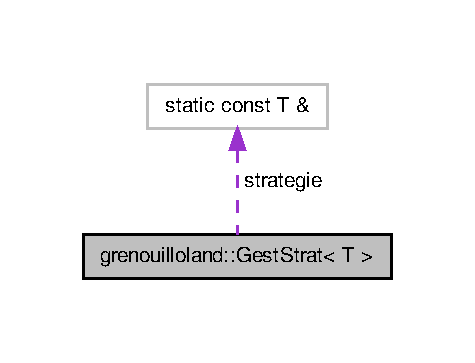
\includegraphics[width=228pt]{classgrenouilloland_1_1GestStrat__coll__graph}
\end{center}
\end{figure}
\subsection*{Attributs publics statiques}
\begin{DoxyCompactItemize}
\item 
static const T \& \hyperlink{classgrenouilloland_1_1GestStrat_afa2982ce94250faed383990231c491bf}{strategie} = T\-::\-Mandataire\-::\-Strategie()
\end{DoxyCompactItemize}


\subsection{Description détaillée}
\subsubsection*{template$<$class T$>$class grenouilloland\-::\-Gest\-Strat$<$ T $>$}

Gest\-Strat$<$\-T$>$ du \hyperlink{classgrenouilloland_1_1Jeu}{Jeu} Grenouilloland. 

\begin{DoxyAuthor}{Auteur}
Beudin.\-Alexandre Dauxais.\-Yann 
\end{DoxyAuthor}
\begin{DoxyDate}{Date}
05.\-01.\-2012
\end{DoxyDate}
Declaration de la classe template \hyperlink{classgrenouilloland_1_1GestStrat}{Gest\-Strat} réprésentant un nénuphar vénéneux du jeu Grenouilloland. 

\subsection{Documentation des données membres}
\hypertarget{classgrenouilloland_1_1GestStrat_afa2982ce94250faed383990231c491bf}{\index{grenouilloland\-::\-Gest\-Strat@{grenouilloland\-::\-Gest\-Strat}!strategie@{strategie}}
\index{strategie@{strategie}!grenouilloland::GestStrat@{grenouilloland\-::\-Gest\-Strat}}
\subsubsection[{strategie}]{\setlength{\rightskip}{0pt plus 5cm}template$<$class T $>$ const T \& {\bf grenouilloland\-::\-Gest\-Strat}$<$ T $>$\-::strategie = T\-::\-Mandataire\-::\-Strategie()\hspace{0.3cm}{\ttfamily [static]}}}\label{classgrenouilloland_1_1GestStrat_afa2982ce94250faed383990231c491bf}
Stratégie gérée par la classe.

La stratégie est fournie par la méthode Strategie() du Mandataire de celle-\/ci. 

La documentation de cette classe a été générée à partir du fichier suivant \-:\begin{DoxyCompactItemize}
\item 
src/modele/include/T\-Gest\-Strat.\-hh\end{DoxyCompactItemize}

\hypertarget{classgrenouilloland_1_1Grenouille}{\section{Référence de la classe grenouilloland\-:\-:Grenouille}
\label{classgrenouilloland_1_1Grenouille}\index{grenouilloland\-::\-Grenouille@{grenouilloland\-::\-Grenouille}}
}


\hyperlink{classgrenouilloland_1_1Grenouille}{Grenouille} du \hyperlink{classgrenouilloland_1_1Jeu}{Jeu} Grenouilloland.  




{\ttfamily \#include $<$Grenouille.\-hh$>$}



Graphe de collaboration de grenouilloland\-:\-:Grenouille\-:
\nopagebreak
\begin{figure}[H]
\begin{center}
\leavevmode
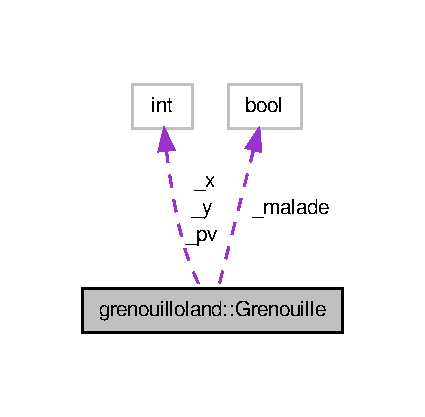
\includegraphics[width=204pt]{classgrenouilloland_1_1Grenouille__coll__graph}
\end{center}
\end{figure}
\subsection*{Classes}
\begin{DoxyCompactItemize}
\item 
class \hyperlink{classgrenouilloland_1_1Grenouille_1_1MandataireEtat}{Mandataire\-Etat}
\begin{DoxyCompactList}\small\item\em \hyperlink{classgrenouilloland_1_1Grenouille_1_1MandataireEtat}{Mandataire\-Etat} de \hyperlink{classgrenouilloland_1_1Grenouille}{Grenouille} du \hyperlink{classgrenouilloland_1_1Jeu}{Jeu} Grenouilloland. \end{DoxyCompactList}\item 
class \hyperlink{classgrenouilloland_1_1Grenouille_1_1MandatairePosition}{Mandataire\-Position}
\begin{DoxyCompactList}\small\item\em \hyperlink{classgrenouilloland_1_1Grenouille_1_1MandatairePosition}{Mandataire\-Position} de \hyperlink{classgrenouilloland_1_1Grenouille}{Grenouille} du \hyperlink{classgrenouilloland_1_1Jeu}{Jeu} Grenouilloland. \end{DoxyCompactList}\end{DoxyCompactItemize}
\subsection*{Fonctions membres publiques}
\begin{DoxyCompactItemize}
\item 
\hyperlink{classgrenouilloland_1_1Grenouille_a326ab4ac092c17f75bae7f966c991f21}{Grenouille} (const unsigned int \&x, const unsigned int \&y)
\item 
const unsigned int \& \hyperlink{classgrenouilloland_1_1Grenouille_afc9b3a8e9454d5172b0f6c7919c39096}{get\-Pv} () const 
\item 
const bool \& \hyperlink{classgrenouilloland_1_1Grenouille_a34a9cbbdbd8ba170c1e417315ef220ca}{get\-Malade} () const 
\item 
const unsigned int \& \hyperlink{classgrenouilloland_1_1Grenouille_ad1e7306d8f1bd838d5d37ec215c1ca38}{get\-X} () const 
\item 
const unsigned int \& \hyperlink{classgrenouilloland_1_1Grenouille_a3110e6b856e7fe92113749c5ee3eb8f1}{get\-Y} () const 
\end{DoxyCompactItemize}
\subsection*{Attributs protégés}
\begin{DoxyCompactItemize}
\item 
unsigned int \hyperlink{classgrenouilloland_1_1Grenouille_a8dc2111b41b87f2c751405841dd73604}{\-\_\-pv}
\item 
bool \hyperlink{classgrenouilloland_1_1Grenouille_a0fbd566d479f7c5b2968606948869b42}{\-\_\-malade}
\item 
unsigned int \hyperlink{classgrenouilloland_1_1Grenouille_ac058265e4d19df895f88d2c485a62eee}{\-\_\-x}
\item 
unsigned int \hyperlink{classgrenouilloland_1_1Grenouille_accbac66bf92efeca1135682eb24c99e7}{\-\_\-y}
\end{DoxyCompactItemize}


\subsection{Description détaillée}
\hyperlink{classgrenouilloland_1_1Grenouille}{Grenouille} du \hyperlink{classgrenouilloland_1_1Jeu}{Jeu} Grenouilloland. 

\begin{DoxyAuthor}{Auteur}
Beudin.\-Alexandre Dauxais.\-Yann 
\end{DoxyAuthor}
\begin{DoxyDate}{Date}
05.\-01.\-2012
\end{DoxyDate}
Declaration de la classe \hyperlink{classgrenouilloland_1_1Grenouille}{Grenouille} réprésentant la grenouille du jeu Grenouilloland. 

\subsection{Documentation des constructeurs et destructeur}
\hypertarget{classgrenouilloland_1_1Grenouille_a326ab4ac092c17f75bae7f966c991f21}{\index{grenouilloland\-::\-Grenouille@{grenouilloland\-::\-Grenouille}!Grenouille@{Grenouille}}
\index{Grenouille@{Grenouille}!grenouilloland::Grenouille@{grenouilloland\-::\-Grenouille}}
\subsubsection[{Grenouille}]{\setlength{\rightskip}{0pt plus 5cm}Grenouille\-::\-Grenouille (
\begin{DoxyParamCaption}
\item[{const unsigned int \&}]{x, }
\item[{const unsigned int \&}]{y}
\end{DoxyParamCaption}
)}}\label{classgrenouilloland_1_1Grenouille_a326ab4ac092c17f75bae7f966c991f21}
Constructeur logique de la grenouille.


\begin{DoxyParams}[1]{Paramètres}
\mbox{\tt in}  & {\em x} & -\/ position de la grenouille sur l'axe x. \\
\hline
\mbox{\tt in}  & {\em y} & -\/ position de la grenouille sur l'axe y. \\
\hline
\end{DoxyParams}


\subsection{Documentation des fonctions membres}
\hypertarget{classgrenouilloland_1_1Grenouille_a34a9cbbdbd8ba170c1e417315ef220ca}{\index{grenouilloland\-::\-Grenouille@{grenouilloland\-::\-Grenouille}!get\-Malade@{get\-Malade}}
\index{get\-Malade@{get\-Malade}!grenouilloland::Grenouille@{grenouilloland\-::\-Grenouille}}
\subsubsection[{get\-Malade}]{\setlength{\rightskip}{0pt plus 5cm}const bool \& Grenouille\-::get\-Malade (
\begin{DoxyParamCaption}
{}
\end{DoxyParamCaption}
) const}}\label{classgrenouilloland_1_1Grenouille_a34a9cbbdbd8ba170c1e417315ef220ca}
Accesseur de l'état de santé de la grenouille.

\begin{DoxyReturn}{Renvoie}
la valeur de \hyperlink{classgrenouilloland_1_1Grenouille_a0fbd566d479f7c5b2968606948869b42}{\-\_\-malade}. 
\end{DoxyReturn}
\hypertarget{classgrenouilloland_1_1Grenouille_afc9b3a8e9454d5172b0f6c7919c39096}{\index{grenouilloland\-::\-Grenouille@{grenouilloland\-::\-Grenouille}!get\-Pv@{get\-Pv}}
\index{get\-Pv@{get\-Pv}!grenouilloland::Grenouille@{grenouilloland\-::\-Grenouille}}
\subsubsection[{get\-Pv}]{\setlength{\rightskip}{0pt plus 5cm}const unsigned int \& Grenouille\-::get\-Pv (
\begin{DoxyParamCaption}
{}
\end{DoxyParamCaption}
) const}}\label{classgrenouilloland_1_1Grenouille_afc9b3a8e9454d5172b0f6c7919c39096}
Accesseur du nombre de pv de la grenouille.

\begin{DoxyReturn}{Renvoie}
la valeur de \hyperlink{classgrenouilloland_1_1Grenouille_a8dc2111b41b87f2c751405841dd73604}{\-\_\-pv}. 
\end{DoxyReturn}
\hypertarget{classgrenouilloland_1_1Grenouille_ad1e7306d8f1bd838d5d37ec215c1ca38}{\index{grenouilloland\-::\-Grenouille@{grenouilloland\-::\-Grenouille}!get\-X@{get\-X}}
\index{get\-X@{get\-X}!grenouilloland::Grenouille@{grenouilloland\-::\-Grenouille}}
\subsubsection[{get\-X}]{\setlength{\rightskip}{0pt plus 5cm}const unsigned int \& Grenouille\-::get\-X (
\begin{DoxyParamCaption}
{}
\end{DoxyParamCaption}
) const}}\label{classgrenouilloland_1_1Grenouille_ad1e7306d8f1bd838d5d37ec215c1ca38}
Accesseur de la position de la grenouille sur l'axe x.

\begin{DoxyReturn}{Renvoie}
la valeur de \hyperlink{classgrenouilloland_1_1Grenouille_ac058265e4d19df895f88d2c485a62eee}{\-\_\-x}. 
\end{DoxyReturn}
\hypertarget{classgrenouilloland_1_1Grenouille_a3110e6b856e7fe92113749c5ee3eb8f1}{\index{grenouilloland\-::\-Grenouille@{grenouilloland\-::\-Grenouille}!get\-Y@{get\-Y}}
\index{get\-Y@{get\-Y}!grenouilloland::Grenouille@{grenouilloland\-::\-Grenouille}}
\subsubsection[{get\-Y}]{\setlength{\rightskip}{0pt plus 5cm}const unsigned int \& Grenouille\-::get\-Y (
\begin{DoxyParamCaption}
{}
\end{DoxyParamCaption}
) const}}\label{classgrenouilloland_1_1Grenouille_a3110e6b856e7fe92113749c5ee3eb8f1}
Accesseur de la position de la grenouille sur l'axe y.

\begin{DoxyReturn}{Renvoie}
la valeur de \hyperlink{classgrenouilloland_1_1Grenouille_accbac66bf92efeca1135682eb24c99e7}{\-\_\-y}. 
\end{DoxyReturn}


\subsection{Documentation des données membres}
\hypertarget{classgrenouilloland_1_1Grenouille_a0fbd566d479f7c5b2968606948869b42}{\index{grenouilloland\-::\-Grenouille@{grenouilloland\-::\-Grenouille}!\-\_\-malade@{\-\_\-malade}}
\index{\-\_\-malade@{\-\_\-malade}!grenouilloland::Grenouille@{grenouilloland\-::\-Grenouille}}
\subsubsection[{\-\_\-malade}]{\setlength{\rightskip}{0pt plus 5cm}bool grenouilloland\-::\-Grenouille\-::\-\_\-malade\hspace{0.3cm}{\ttfamily [protected]}}}\label{classgrenouilloland_1_1Grenouille_a0fbd566d479f7c5b2968606948869b42}
\hyperlink{classgrenouilloland_1_1Etat}{Etat} de santé de la grenouille. \hypertarget{classgrenouilloland_1_1Grenouille_a8dc2111b41b87f2c751405841dd73604}{\index{grenouilloland\-::\-Grenouille@{grenouilloland\-::\-Grenouille}!\-\_\-pv@{\-\_\-pv}}
\index{\-\_\-pv@{\-\_\-pv}!grenouilloland::Grenouille@{grenouilloland\-::\-Grenouille}}
\subsubsection[{\-\_\-pv}]{\setlength{\rightskip}{0pt plus 5cm}unsigned int grenouilloland\-::\-Grenouille\-::\-\_\-pv\hspace{0.3cm}{\ttfamily [protected]}}}\label{classgrenouilloland_1_1Grenouille_a8dc2111b41b87f2c751405841dd73604}
Nombre de pv de la grenouille. \hypertarget{classgrenouilloland_1_1Grenouille_ac058265e4d19df895f88d2c485a62eee}{\index{grenouilloland\-::\-Grenouille@{grenouilloland\-::\-Grenouille}!\-\_\-x@{\-\_\-x}}
\index{\-\_\-x@{\-\_\-x}!grenouilloland::Grenouille@{grenouilloland\-::\-Grenouille}}
\subsubsection[{\-\_\-x}]{\setlength{\rightskip}{0pt plus 5cm}unsigned int grenouilloland\-::\-Grenouille\-::\-\_\-x\hspace{0.3cm}{\ttfamily [protected]}}}\label{classgrenouilloland_1_1Grenouille_ac058265e4d19df895f88d2c485a62eee}
Position de la grenouille sur l'axe x. \hypertarget{classgrenouilloland_1_1Grenouille_accbac66bf92efeca1135682eb24c99e7}{\index{grenouilloland\-::\-Grenouille@{grenouilloland\-::\-Grenouille}!\-\_\-y@{\-\_\-y}}
\index{\-\_\-y@{\-\_\-y}!grenouilloland::Grenouille@{grenouilloland\-::\-Grenouille}}
\subsubsection[{\-\_\-y}]{\setlength{\rightskip}{0pt plus 5cm}unsigned int grenouilloland\-::\-Grenouille\-::\-\_\-y\hspace{0.3cm}{\ttfamily [protected]}}}\label{classgrenouilloland_1_1Grenouille_accbac66bf92efeca1135682eb24c99e7}
Position de la grenouille sur l'axe y. 

La documentation de cette classe a été générée à partir des fichiers suivants \-:\begin{DoxyCompactItemize}
\item 
src/modele/include/Grenouille.\-hh\item 
src/modele/Grenouille.\-cpp\end{DoxyCompactItemize}

\hypertarget{classgrenouilloland_1_1GrenouillolandGraphique}{\section{Référence de la classe grenouilloland\-:\-:Grenouilloland\-Graphique}
\label{classgrenouilloland_1_1GrenouillolandGraphique}\index{grenouilloland\-::\-Grenouilloland\-Graphique@{grenouilloland\-::\-Grenouilloland\-Graphique}}
}


Representation graphique du \hyperlink{classgrenouilloland_1_1Jeu}{Jeu} grenouilloland.  




{\ttfamily \#include $<$Grenouilloland\-Graphique.\-hh$>$}



Graphe d'héritage de grenouilloland\-:\-:Grenouilloland\-Graphique\-:
\nopagebreak
\begin{figure}[H]
\begin{center}
\leavevmode
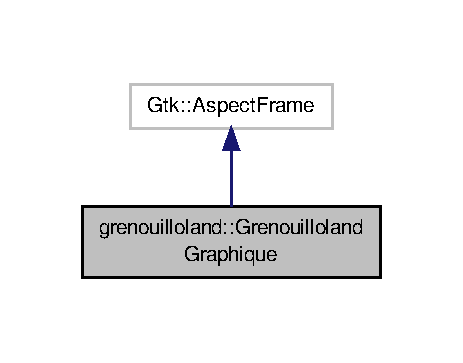
\includegraphics[width=222pt]{classgrenouilloland_1_1GrenouillolandGraphique__inherit__graph}
\end{center}
\end{figure}


Graphe de collaboration de grenouilloland\-:\-:Grenouilloland\-Graphique\-:
\nopagebreak
\begin{figure}[H]
\begin{center}
\leavevmode
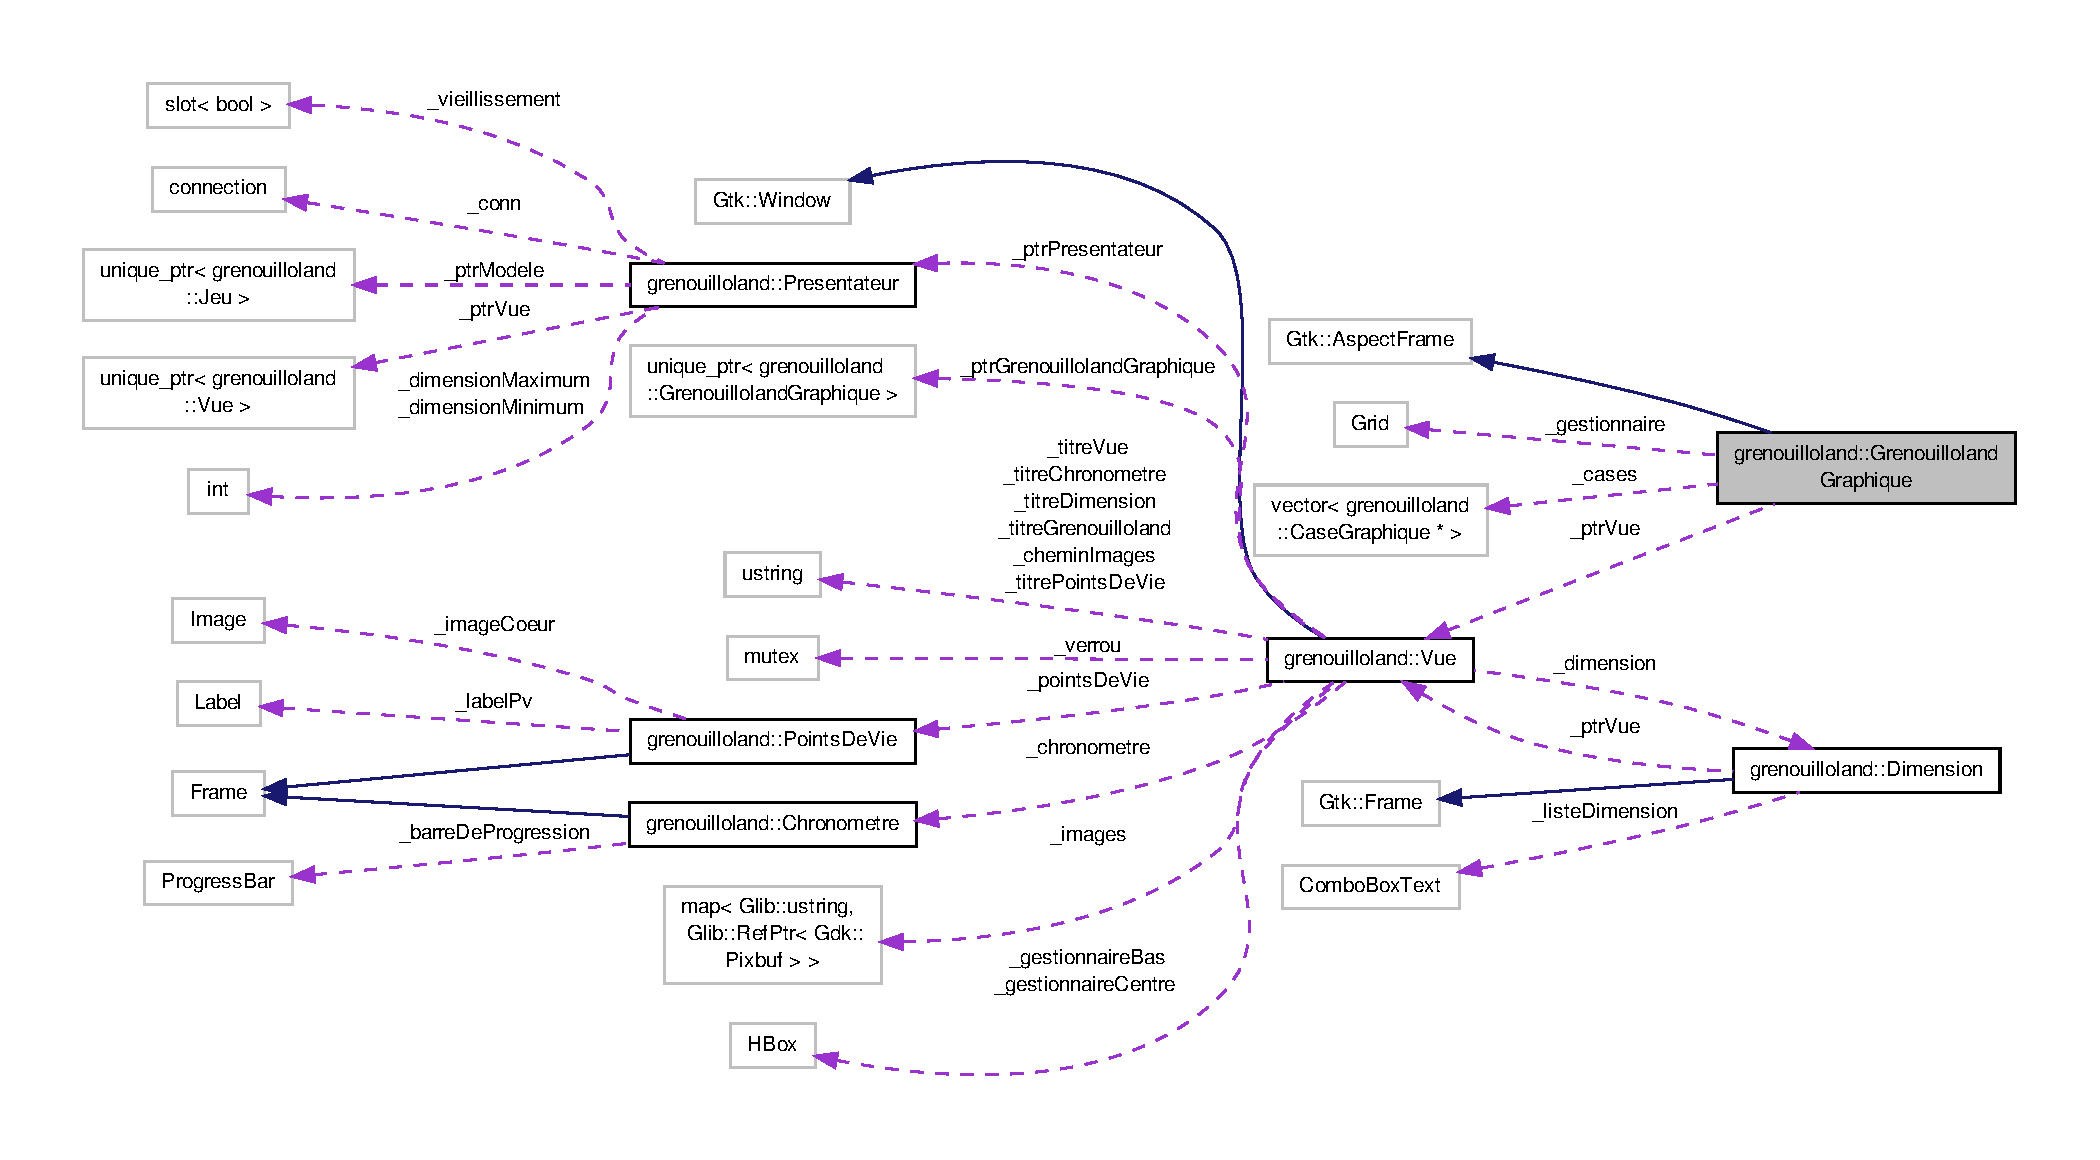
\includegraphics[width=350pt]{classgrenouilloland_1_1GrenouillolandGraphique__coll__graph}
\end{center}
\end{figure}
\subsection*{Fonctions membres publiques}
\begin{DoxyCompactItemize}
\item 
\hyperlink{classgrenouilloland_1_1GrenouillolandGraphique_a97d352b5fdf2875f4d86d68c86579547}{Grenouilloland\-Graphique} (const Glib\-::ustring \&titre, \hyperlink{classgrenouilloland_1_1Vue}{Vue} \&vue)
\item 
const \hyperlink{classgrenouilloland_1_1Vue}{Vue} \& \hyperlink{classgrenouilloland_1_1GrenouillolandGraphique_a7b19495a473e950ed6ff6e9b3d307abc}{lire\-Vue} () const 
\end{DoxyCompactItemize}
\subsection*{Fonctions membres protégées}
\begin{DoxyCompactItemize}
\item 
\hyperlink{classgrenouilloland_1_1Vue}{Vue} \& \hyperlink{classgrenouilloland_1_1GrenouillolandGraphique_a077a9aa314172f04d4fecee498c5a37a}{lire\-Vue\-Modifiable} ()
\item 
void \hyperlink{classgrenouilloland_1_1GrenouillolandGraphique_a456350eac30419edfab5a9e37d49da1b}{mettre\-A\-Jour} (const \hyperlink{classgrenouilloland_1_1Presentateur}{Presentateur} \&presentateur)
\end{DoxyCompactItemize}
\subsection*{Attributs protégés}
\begin{DoxyCompactItemize}
\item 
\hyperlink{classgrenouilloland_1_1Vue}{Vue} $\ast$const \hyperlink{classgrenouilloland_1_1GrenouillolandGraphique_aa0fe0c7d9e9cd676b8ce62a40ab97c62}{\-\_\-ptr\-Vue}
\item 
Gtk\-::\-Grid \hyperlink{classgrenouilloland_1_1GrenouillolandGraphique_a71036819a9bba19e6ecee48cf7acc00b}{\-\_\-gestionnaire}
\item 
std\-::vector$<$ \hyperlink{classgrenouilloland_1_1CaseGraphique}{Case\-Graphique} $\ast$ $>$ \hyperlink{classgrenouilloland_1_1GrenouillolandGraphique_ab4d1dbe72f42279511f2ccbd171bbffe}{\-\_\-cases}
\end{DoxyCompactItemize}
\subsection*{Amis}
\begin{DoxyCompactItemize}
\item 
class \hyperlink{classgrenouilloland_1_1GrenouillolandGraphique_adc3b1810b8d3988a7832f57c330fe4fd}{Vue}
\item 
class \hyperlink{classgrenouilloland_1_1GrenouillolandGraphique_ac12b0ba9ebe667c8408ac35bf21598e8}{Case\-Graphique}
\end{DoxyCompactItemize}


\subsection{Description détaillée}
Representation graphique du \hyperlink{classgrenouilloland_1_1Jeu}{Jeu} grenouilloland. 

\begin{DoxyAuthor}{Auteur}
Yann Dauxais 

Alexandre Beudin 
\end{DoxyAuthor}
\begin{DoxyDate}{Date}
6.\-1.\-2013
\end{DoxyDate}
Declaration de la classe \hyperlink{classgrenouilloland_1_1GrenouillolandGraphique}{Grenouilloland\-Graphique} representant le plateau du \hyperlink{classgrenouilloland_1_1Jeu}{Jeu} Grenouilloland.

\begin{DoxyNote}{Note}
Une instance de cette classe ne peut être dupliquée. 
\end{DoxyNote}


\subsection{Documentation des constructeurs et destructeur}
\hypertarget{classgrenouilloland_1_1GrenouillolandGraphique_a97d352b5fdf2875f4d86d68c86579547}{\index{grenouilloland\-::\-Grenouilloland\-Graphique@{grenouilloland\-::\-Grenouilloland\-Graphique}!Grenouilloland\-Graphique@{Grenouilloland\-Graphique}}
\index{Grenouilloland\-Graphique@{Grenouilloland\-Graphique}!grenouilloland::GrenouillolandGraphique@{grenouilloland\-::\-Grenouilloland\-Graphique}}
\subsubsection[{Grenouilloland\-Graphique}]{\setlength{\rightskip}{0pt plus 5cm}Grenouilloland\-Graphique\-::\-Grenouilloland\-Graphique (
\begin{DoxyParamCaption}
\item[{const Glib\-::ustring \&}]{titre, }
\item[{{\bf Vue} \&}]{vue}
\end{DoxyParamCaption}
)}}\label{classgrenouilloland_1_1GrenouillolandGraphique_a97d352b5fdf2875f4d86d68c86579547}
Constructeur logique.


\begin{DoxyParams}[1]{Paramètres}
\mbox{\tt in}  & {\em titre} & -\/ le titre du contour. \\
\hline
\mbox{\tt in,out}  & {\em vue} & -\/ la valeur de \hyperlink{classgrenouilloland_1_1GrenouillolandGraphique_aa0fe0c7d9e9cd676b8ce62a40ab97c62}{\-\_\-ptr\-Vue}. \\
\hline
\end{DoxyParams}


\subsection{Documentation des fonctions membres}
\hypertarget{classgrenouilloland_1_1GrenouillolandGraphique_a7b19495a473e950ed6ff6e9b3d307abc}{\index{grenouilloland\-::\-Grenouilloland\-Graphique@{grenouilloland\-::\-Grenouilloland\-Graphique}!lire\-Vue@{lire\-Vue}}
\index{lire\-Vue@{lire\-Vue}!grenouilloland::GrenouillolandGraphique@{grenouilloland\-::\-Grenouilloland\-Graphique}}
\subsubsection[{lire\-Vue}]{\setlength{\rightskip}{0pt plus 5cm}const {\bf Vue} \& Grenouilloland\-Graphique\-::lire\-Vue (
\begin{DoxyParamCaption}
{}
\end{DoxyParamCaption}
) const}}\label{classgrenouilloland_1_1GrenouillolandGraphique_a7b19495a473e950ed6ff6e9b3d307abc}
Accesseur.

\begin{DoxyReturn}{Renvoie}
la valeur de \hyperlink{classgrenouilloland_1_1GrenouillolandGraphique_aa0fe0c7d9e9cd676b8ce62a40ab97c62}{\-\_\-ptr\-Vue}. 
\end{DoxyReturn}
\hypertarget{classgrenouilloland_1_1GrenouillolandGraphique_a077a9aa314172f04d4fecee498c5a37a}{\index{grenouilloland\-::\-Grenouilloland\-Graphique@{grenouilloland\-::\-Grenouilloland\-Graphique}!lire\-Vue\-Modifiable@{lire\-Vue\-Modifiable}}
\index{lire\-Vue\-Modifiable@{lire\-Vue\-Modifiable}!grenouilloland::GrenouillolandGraphique@{grenouilloland\-::\-Grenouilloland\-Graphique}}
\subsubsection[{lire\-Vue\-Modifiable}]{\setlength{\rightskip}{0pt plus 5cm}{\bf Vue} \& Grenouilloland\-Graphique\-::lire\-Vue\-Modifiable (
\begin{DoxyParamCaption}
{}
\end{DoxyParamCaption}
)\hspace{0.3cm}{\ttfamily [protected]}}}\label{classgrenouilloland_1_1GrenouillolandGraphique_a077a9aa314172f04d4fecee498c5a37a}
Accesseur.

\begin{DoxyReturn}{Renvoie}
la valeur de \hyperlink{classgrenouilloland_1_1GrenouillolandGraphique_aa0fe0c7d9e9cd676b8ce62a40ab97c62}{\-\_\-ptr\-Vue}. 
\end{DoxyReturn}
\hypertarget{classgrenouilloland_1_1GrenouillolandGraphique_a456350eac30419edfab5a9e37d49da1b}{\index{grenouilloland\-::\-Grenouilloland\-Graphique@{grenouilloland\-::\-Grenouilloland\-Graphique}!mettre\-A\-Jour@{mettre\-A\-Jour}}
\index{mettre\-A\-Jour@{mettre\-A\-Jour}!grenouilloland::GrenouillolandGraphique@{grenouilloland\-::\-Grenouilloland\-Graphique}}
\subsubsection[{mettre\-A\-Jour}]{\setlength{\rightskip}{0pt plus 5cm}void Grenouilloland\-Graphique\-::mettre\-A\-Jour (
\begin{DoxyParamCaption}
\item[{const {\bf Presentateur} \&}]{presentateur}
\end{DoxyParamCaption}
)\hspace{0.3cm}{\ttfamily [protected]}}}\label{classgrenouilloland_1_1GrenouillolandGraphique_a456350eac30419edfab5a9e37d49da1b}
Met a jour l'ensemble des cases graphiques de ce jeu graphique.


\begin{DoxyParams}[1]{Paramètres}
\mbox{\tt in}  & {\em presentateur} & -\/ le presentateur a invoquer.\\
\hline
\end{DoxyParams}
\begin{DoxyNote}{Note}
La vue doit etre verrouillee pour pouvoir invoquer cette methode. 
\end{DoxyNote}


\subsection{Documentation des fonctions amies et associées}
\hypertarget{classgrenouilloland_1_1GrenouillolandGraphique_ac12b0ba9ebe667c8408ac35bf21598e8}{\index{grenouilloland\-::\-Grenouilloland\-Graphique@{grenouilloland\-::\-Grenouilloland\-Graphique}!Case\-Graphique@{Case\-Graphique}}
\index{Case\-Graphique@{Case\-Graphique}!grenouilloland::GrenouillolandGraphique@{grenouilloland\-::\-Grenouilloland\-Graphique}}
\subsubsection[{Case\-Graphique}]{\setlength{\rightskip}{0pt plus 5cm}friend class {\bf Case\-Graphique}\hspace{0.3cm}{\ttfamily [friend]}}}\label{classgrenouilloland_1_1GrenouillolandGraphique_ac12b0ba9ebe667c8408ac35bf21598e8}
Declaration d'amitié. \hypertarget{classgrenouilloland_1_1GrenouillolandGraphique_adc3b1810b8d3988a7832f57c330fe4fd}{\index{grenouilloland\-::\-Grenouilloland\-Graphique@{grenouilloland\-::\-Grenouilloland\-Graphique}!Vue@{Vue}}
\index{Vue@{Vue}!grenouilloland::GrenouillolandGraphique@{grenouilloland\-::\-Grenouilloland\-Graphique}}
\subsubsection[{Vue}]{\setlength{\rightskip}{0pt plus 5cm}friend class {\bf Vue}\hspace{0.3cm}{\ttfamily [friend]}}}\label{classgrenouilloland_1_1GrenouillolandGraphique_adc3b1810b8d3988a7832f57c330fe4fd}
Declaration d'amitié. 

\subsection{Documentation des données membres}
\hypertarget{classgrenouilloland_1_1GrenouillolandGraphique_ab4d1dbe72f42279511f2ccbd171bbffe}{\index{grenouilloland\-::\-Grenouilloland\-Graphique@{grenouilloland\-::\-Grenouilloland\-Graphique}!\-\_\-cases@{\-\_\-cases}}
\index{\-\_\-cases@{\-\_\-cases}!grenouilloland::GrenouillolandGraphique@{grenouilloland\-::\-Grenouilloland\-Graphique}}
\subsubsection[{\-\_\-cases}]{\setlength{\rightskip}{0pt plus 5cm}std\-::vector$<$ {\bf Case\-Graphique}$\ast$ $>$ grenouilloland\-::\-Grenouilloland\-Graphique\-::\-\_\-cases\hspace{0.3cm}{\ttfamily [protected]}}}\label{classgrenouilloland_1_1GrenouillolandGraphique_ab4d1dbe72f42279511f2ccbd171bbffe}
Cases graphiques de cette representation graphique du jeu grenouilloland. \hypertarget{classgrenouilloland_1_1GrenouillolandGraphique_a71036819a9bba19e6ecee48cf7acc00b}{\index{grenouilloland\-::\-Grenouilloland\-Graphique@{grenouilloland\-::\-Grenouilloland\-Graphique}!\-\_\-gestionnaire@{\-\_\-gestionnaire}}
\index{\-\_\-gestionnaire@{\-\_\-gestionnaire}!grenouilloland::GrenouillolandGraphique@{grenouilloland\-::\-Grenouilloland\-Graphique}}
\subsubsection[{\-\_\-gestionnaire}]{\setlength{\rightskip}{0pt plus 5cm}Gtk\-::\-Grid grenouilloland\-::\-Grenouilloland\-Graphique\-::\-\_\-gestionnaire\hspace{0.3cm}{\ttfamily [protected]}}}\label{classgrenouilloland_1_1GrenouillolandGraphique_a71036819a9bba19e6ecee48cf7acc00b}
Gestionnaire de mise en forme de ce plateau. \hypertarget{classgrenouilloland_1_1GrenouillolandGraphique_aa0fe0c7d9e9cd676b8ce62a40ab97c62}{\index{grenouilloland\-::\-Grenouilloland\-Graphique@{grenouilloland\-::\-Grenouilloland\-Graphique}!\-\_\-ptr\-Vue@{\-\_\-ptr\-Vue}}
\index{\-\_\-ptr\-Vue@{\-\_\-ptr\-Vue}!grenouilloland::GrenouillolandGraphique@{grenouilloland\-::\-Grenouilloland\-Graphique}}
\subsubsection[{\-\_\-ptr\-Vue}]{\setlength{\rightskip}{0pt plus 5cm}{\bf Vue}$\ast$ const grenouilloland\-::\-Grenouilloland\-Graphique\-::\-\_\-ptr\-Vue\hspace{0.3cm}{\ttfamily [protected]}}}\label{classgrenouilloland_1_1GrenouillolandGraphique_aa0fe0c7d9e9cd676b8ce62a40ab97c62}
Unique vue proprietaire de cette generation. 

La documentation de cette classe a été générée à partir des fichiers suivants \-:\begin{DoxyCompactItemize}
\item 
src/vue/include/Grenouilloland\-Graphique.\-hh\item 
src/vue/Grenouilloland\-Graphique.\-cpp\end{DoxyCompactItemize}

\hypertarget{classgrenouilloland_1_1Jeu}{\section{Référence de la classe grenouilloland\-:\-:Jeu}
\label{classgrenouilloland_1_1Jeu}\index{grenouilloland\-::\-Jeu@{grenouilloland\-::\-Jeu}}
}


\hyperlink{classgrenouilloland_1_1Jeu}{Jeu} du \hyperlink{classgrenouilloland_1_1Jeu}{Jeu} Grenouilloland.  




{\ttfamily \#include $<$Jeu.\-hh$>$}



Graphe de collaboration de grenouilloland\-:\-:Jeu\-:
\nopagebreak
\begin{figure}[H]
\begin{center}
\leavevmode
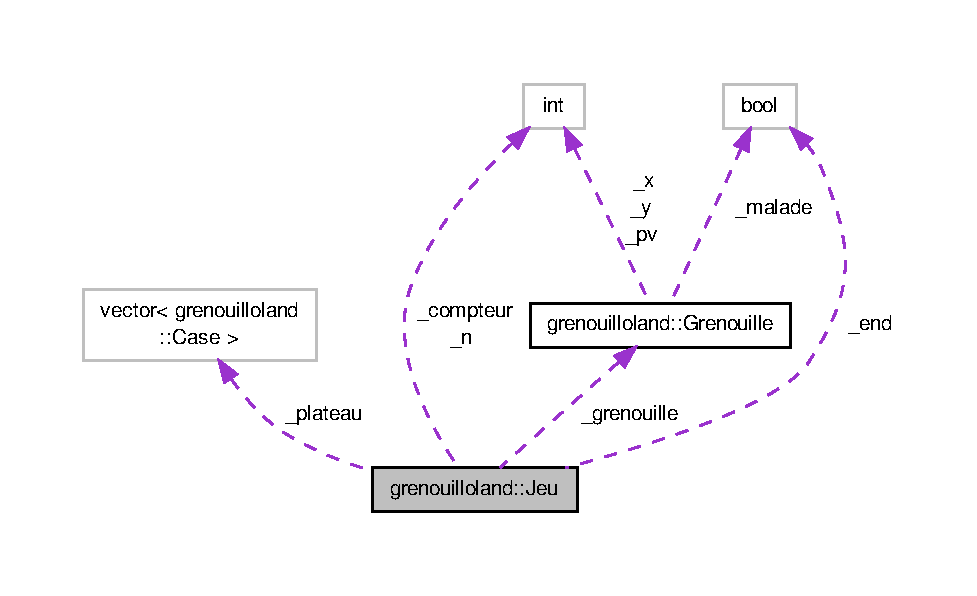
\includegraphics[width=350pt]{classgrenouilloland_1_1Jeu__coll__graph}
\end{center}
\end{figure}
\subsection*{Classes}
\begin{DoxyCompactItemize}
\item 
class \hyperlink{classgrenouilloland_1_1Jeu_1_1Mandataire}{Mandataire}
\begin{DoxyCompactList}\small\item\em \hyperlink{classgrenouilloland_1_1Jeu_1_1Mandataire}{Mandataire} du \hyperlink{classgrenouilloland_1_1Jeu}{Jeu}. \end{DoxyCompactList}\end{DoxyCompactItemize}
\subsection*{Fonctions membres publiques}
\begin{DoxyCompactItemize}
\item 
\hyperlink{classgrenouilloland_1_1Jeu_aa17e547858c8e5d805c630dd52709599}{Jeu} (const int \&n)
\item 
const int \& \hyperlink{classgrenouilloland_1_1Jeu_ad0212b9c81ad43fa588275b5352e2f10}{lire\-Dimension} () const 
\item 
const unsigned int \& \hyperlink{classgrenouilloland_1_1Jeu_aaf16fe8116cec0e81936c4afbbaf9d9b}{lire\-Compteur} () const 
\item 
const \hyperlink{classgrenouilloland_1_1Case}{Case} \& \hyperlink{classgrenouilloland_1_1Jeu_a86292514d1a52166e63b54f09992ce93}{lire\-Case} (const int \&ligne, const int \&colonne) const 
\item 
const unsigned int \& \hyperlink{classgrenouilloland_1_1Jeu_ad3e1ac4ffca6a1f360de9d3dae2f02f6}{lire\-Pv\-Grenouille} () const 
\item 
bool \hyperlink{classgrenouilloland_1_1Jeu_a6317f289086e77fed2c4555c38fa86af}{grenouille\-Malade} () const 
\item 
bool \hyperlink{classgrenouilloland_1_1Jeu_a3a90f0bd8b1dd81ee311fd20b2c3df31}{presence\-Grenouille} (const unsigned int \&ligne, const unsigned int \&colonne) const 
\item 
bool \hyperlink{classgrenouilloland_1_1Jeu_aa95a6941d6b5fe55fe775824dfe7c1b7}{end} () const 
\item 
\hyperlink{classgrenouilloland_1_1Element}{Element} $\ast$ \hyperlink{classgrenouilloland_1_1Jeu_a0bee5ac205c6fa11f71e237f2d1b8a02}{nenuphar\-Aleatoire} () const 
\end{DoxyCompactItemize}
\subsection*{Fonctions membres protégées}
\begin{DoxyCompactItemize}
\item 
void \hyperlink{classgrenouilloland_1_1Jeu_ab07fc3cd7186b844201d3e7639dcdf37}{reinitialiser} ()
\item 
void \hyperlink{classgrenouilloland_1_1Jeu_a98de76a91961f5c12bb1df678484dafa}{lancer\-Partie} ()
\item 
bool \hyperlink{classgrenouilloland_1_1Jeu_aec511079bde27f924e47db40239bf2f4}{deplacer\-Grenouille} (const int \&x, const int \&y)
\item 
void \hyperlink{classgrenouilloland_1_1Jeu_aed1eb1f7ece1d95617d168f84827dacd}{creer\-Chemin} ()
\item 
bool \hyperlink{classgrenouilloland_1_1Jeu_ae64660044f52c37b9283ed9538cc02df}{verif\-Etat} ()
\item 
bool \hyperlink{classgrenouilloland_1_1Jeu_a4052316bd896fdf6dbec94e03a3ad7aa}{vieillissement} ()
\end{DoxyCompactItemize}
\subsection*{Attributs protégés}
\begin{DoxyCompactItemize}
\item 
\hyperlink{classgrenouilloland_1_1Grenouille}{Grenouille} \hyperlink{classgrenouilloland_1_1Jeu_a411e399b5c5e63bc2c8890dbd0f0a21a}{\-\_\-grenouille}
\item 
std\-::vector$<$ \hyperlink{classgrenouilloland_1_1Case}{Case} $>$ \hyperlink{classgrenouilloland_1_1Jeu_a868edb9c732e86197a14cef627852648}{\-\_\-plateau}
\item 
int \hyperlink{classgrenouilloland_1_1Jeu_ab30a76105853c15cc67ef86d20dec98f}{\-\_\-n}
\item 
bool \hyperlink{classgrenouilloland_1_1Jeu_a2b1ca540559752ed171103258be5a58e}{\-\_\-end}
\item 
unsigned int \hyperlink{classgrenouilloland_1_1Jeu_acffeba39357d08306c91064a766b6e7d}{\-\_\-compteur}
\end{DoxyCompactItemize}


\subsection{Description détaillée}
\hyperlink{classgrenouilloland_1_1Jeu}{Jeu} du \hyperlink{classgrenouilloland_1_1Jeu}{Jeu} Grenouilloland. 

\begin{DoxyAuthor}{Auteur}
Beudin.\-Alexandre Dauxais.\-Yann 
\end{DoxyAuthor}
\begin{DoxyDate}{Date}
05.\-01.\-2012
\end{DoxyDate}
Declaration de la classe \hyperlink{classgrenouilloland_1_1Jeu}{Jeu} réprésentant le plateau du jeu Grenouilloland. 

\subsection{Documentation des constructeurs et destructeur}
\hypertarget{classgrenouilloland_1_1Jeu_aa17e547858c8e5d805c630dd52709599}{\index{grenouilloland\-::\-Jeu@{grenouilloland\-::\-Jeu}!Jeu@{Jeu}}
\index{Jeu@{Jeu}!grenouilloland::Jeu@{grenouilloland\-::\-Jeu}}
\subsubsection[{Jeu}]{\setlength{\rightskip}{0pt plus 5cm}Jeu\-::\-Jeu (
\begin{DoxyParamCaption}
\item[{const int \&}]{n}
\end{DoxyParamCaption}
)}}\label{classgrenouilloland_1_1Jeu_aa17e547858c8e5d805c630dd52709599}
Constructeur logique du jeu.


\begin{DoxyParams}[1]{Paramètres}
\mbox{\tt in}  & {\em n} & -\/ taille du plateau de dimension n$\ast$n. \\
\hline
\end{DoxyParams}


\subsection{Documentation des fonctions membres}
\hypertarget{classgrenouilloland_1_1Jeu_aed1eb1f7ece1d95617d168f84827dacd}{\index{grenouilloland\-::\-Jeu@{grenouilloland\-::\-Jeu}!creer\-Chemin@{creer\-Chemin}}
\index{creer\-Chemin@{creer\-Chemin}!grenouilloland::Jeu@{grenouilloland\-::\-Jeu}}
\subsubsection[{creer\-Chemin}]{\setlength{\rightskip}{0pt plus 5cm}void Jeu\-::creer\-Chemin (
\begin{DoxyParamCaption}
{}
\end{DoxyParamCaption}
)\hspace{0.3cm}{\ttfamily [protected]}}}\label{classgrenouilloland_1_1Jeu_aed1eb1f7ece1d95617d168f84827dacd}
Création de chemins entre la grenouille et la case d'arrivée. \hypertarget{classgrenouilloland_1_1Jeu_aec511079bde27f924e47db40239bf2f4}{\index{grenouilloland\-::\-Jeu@{grenouilloland\-::\-Jeu}!deplacer\-Grenouille@{deplacer\-Grenouille}}
\index{deplacer\-Grenouille@{deplacer\-Grenouille}!grenouilloland::Jeu@{grenouilloland\-::\-Jeu}}
\subsubsection[{deplacer\-Grenouille}]{\setlength{\rightskip}{0pt plus 5cm}bool Jeu\-::deplacer\-Grenouille (
\begin{DoxyParamCaption}
\item[{const int \&}]{x, }
\item[{const int \&}]{y}
\end{DoxyParamCaption}
)\hspace{0.3cm}{\ttfamily [protected]}}}\label{classgrenouilloland_1_1Jeu_aec511079bde27f924e47db40239bf2f4}
Déplacement de la grenouille.


\begin{DoxyParams}[1]{Paramètres}
\mbox{\tt in}  & {\em x} & -\/ position de la grenouille sur l'axe x. \\
\hline
\mbox{\tt in}  & {\em y} & -\/ position de la grenouille sur l'axe y.\\
\hline
\end{DoxyParams}
\begin{DoxyReturn}{Renvoie}
true si le déplacement a été effectué, false sinon. 
\end{DoxyReturn}
\hypertarget{classgrenouilloland_1_1Jeu_aa95a6941d6b5fe55fe775824dfe7c1b7}{\index{grenouilloland\-::\-Jeu@{grenouilloland\-::\-Jeu}!end@{end}}
\index{end@{end}!grenouilloland::Jeu@{grenouilloland\-::\-Jeu}}
\subsubsection[{end}]{\setlength{\rightskip}{0pt plus 5cm}bool Jeu\-::end (
\begin{DoxyParamCaption}
{}
\end{DoxyParamCaption}
) const}}\label{classgrenouilloland_1_1Jeu_aa95a6941d6b5fe55fe775824dfe7c1b7}
Accesseur de l'état de fin du jeu.

\begin{DoxyReturn}{Renvoie}
la valeur de \hyperlink{classgrenouilloland_1_1Jeu_a2b1ca540559752ed171103258be5a58e}{\-\_\-end}. 
\end{DoxyReturn}
\hypertarget{classgrenouilloland_1_1Jeu_a6317f289086e77fed2c4555c38fa86af}{\index{grenouilloland\-::\-Jeu@{grenouilloland\-::\-Jeu}!grenouille\-Malade@{grenouille\-Malade}}
\index{grenouille\-Malade@{grenouille\-Malade}!grenouilloland::Jeu@{grenouilloland\-::\-Jeu}}
\subsubsection[{grenouille\-Malade}]{\setlength{\rightskip}{0pt plus 5cm}bool Jeu\-::grenouille\-Malade (
\begin{DoxyParamCaption}
{}
\end{DoxyParamCaption}
) const}}\label{classgrenouilloland_1_1Jeu_a6317f289086e77fed2c4555c38fa86af}
Accesseur de l'état de santé de la grenouille.

\begin{DoxyReturn}{Renvoie}
la valeur de l'état de santé de la grenouille. 
\end{DoxyReturn}
\hypertarget{classgrenouilloland_1_1Jeu_a98de76a91961f5c12bb1df678484dafa}{\index{grenouilloland\-::\-Jeu@{grenouilloland\-::\-Jeu}!lancer\-Partie@{lancer\-Partie}}
\index{lancer\-Partie@{lancer\-Partie}!grenouilloland::Jeu@{grenouilloland\-::\-Jeu}}
\subsubsection[{lancer\-Partie}]{\setlength{\rightskip}{0pt plus 5cm}void Jeu\-::lancer\-Partie (
\begin{DoxyParamCaption}
{}
\end{DoxyParamCaption}
)\hspace{0.3cm}{\ttfamily [protected]}}}\label{classgrenouilloland_1_1Jeu_a98de76a91961f5c12bb1df678484dafa}
Lancement de la partie. \hypertarget{classgrenouilloland_1_1Jeu_a86292514d1a52166e63b54f09992ce93}{\index{grenouilloland\-::\-Jeu@{grenouilloland\-::\-Jeu}!lire\-Case@{lire\-Case}}
\index{lire\-Case@{lire\-Case}!grenouilloland::Jeu@{grenouilloland\-::\-Jeu}}
\subsubsection[{lire\-Case}]{\setlength{\rightskip}{0pt plus 5cm}const {\bf Case} \& Jeu\-::lire\-Case (
\begin{DoxyParamCaption}
\item[{const int \&}]{ligne, }
\item[{const int \&}]{colonne}
\end{DoxyParamCaption}
) const}}\label{classgrenouilloland_1_1Jeu_a86292514d1a52166e63b54f09992ce93}
Accesseur d'une case du plateau.


\begin{DoxyParams}[1]{Paramètres}
\mbox{\tt in}  & {\em ligne} & -\/ ligne de la case du plateau. \\
\hline
\mbox{\tt in}  & {\em colonne} & -\/ colonne de la case du plateau.\\
\hline
\end{DoxyParams}
\begin{DoxyReturn}{Renvoie}
référence constante sur une case du plateau. 
\end{DoxyReturn}
\hypertarget{classgrenouilloland_1_1Jeu_aaf16fe8116cec0e81936c4afbbaf9d9b}{\index{grenouilloland\-::\-Jeu@{grenouilloland\-::\-Jeu}!lire\-Compteur@{lire\-Compteur}}
\index{lire\-Compteur@{lire\-Compteur}!grenouilloland::Jeu@{grenouilloland\-::\-Jeu}}
\subsubsection[{lire\-Compteur}]{\setlength{\rightskip}{0pt plus 5cm}const unsigned int \& Jeu\-::lire\-Compteur (
\begin{DoxyParamCaption}
{}
\end{DoxyParamCaption}
) const}}\label{classgrenouilloland_1_1Jeu_aaf16fe8116cec0e81936c4afbbaf9d9b}
Accesseur du compteur.

\begin{DoxyReturn}{Renvoie}
la valeur de \hyperlink{classgrenouilloland_1_1Jeu_acffeba39357d08306c91064a766b6e7d}{\-\_\-compteur}. 
\end{DoxyReturn}
\hypertarget{classgrenouilloland_1_1Jeu_ad0212b9c81ad43fa588275b5352e2f10}{\index{grenouilloland\-::\-Jeu@{grenouilloland\-::\-Jeu}!lire\-Dimension@{lire\-Dimension}}
\index{lire\-Dimension@{lire\-Dimension}!grenouilloland::Jeu@{grenouilloland\-::\-Jeu}}
\subsubsection[{lire\-Dimension}]{\setlength{\rightskip}{0pt plus 5cm}const int \& Jeu\-::lire\-Dimension (
\begin{DoxyParamCaption}
{}
\end{DoxyParamCaption}
) const}}\label{classgrenouilloland_1_1Jeu_ad0212b9c81ad43fa588275b5352e2f10}
Accesseur de la dimension du plateau.

\begin{DoxyReturn}{Renvoie}
la valeur de \hyperlink{classgrenouilloland_1_1Jeu_ab30a76105853c15cc67ef86d20dec98f}{\-\_\-n}. 
\end{DoxyReturn}
\hypertarget{classgrenouilloland_1_1Jeu_ad3e1ac4ffca6a1f360de9d3dae2f02f6}{\index{grenouilloland\-::\-Jeu@{grenouilloland\-::\-Jeu}!lire\-Pv\-Grenouille@{lire\-Pv\-Grenouille}}
\index{lire\-Pv\-Grenouille@{lire\-Pv\-Grenouille}!grenouilloland::Jeu@{grenouilloland\-::\-Jeu}}
\subsubsection[{lire\-Pv\-Grenouille}]{\setlength{\rightskip}{0pt plus 5cm}const unsigned int \& Jeu\-::lire\-Pv\-Grenouille (
\begin{DoxyParamCaption}
{}
\end{DoxyParamCaption}
) const}}\label{classgrenouilloland_1_1Jeu_ad3e1ac4ffca6a1f360de9d3dae2f02f6}
Accesseur du nombre de pv de la grenouille.

\begin{DoxyReturn}{Renvoie}
nombre de pv de la grenouille. 
\end{DoxyReturn}
\hypertarget{classgrenouilloland_1_1Jeu_a0bee5ac205c6fa11f71e237f2d1b8a02}{\index{grenouilloland\-::\-Jeu@{grenouilloland\-::\-Jeu}!nenuphar\-Aleatoire@{nenuphar\-Aleatoire}}
\index{nenuphar\-Aleatoire@{nenuphar\-Aleatoire}!grenouilloland::Jeu@{grenouilloland\-::\-Jeu}}
\subsubsection[{nenuphar\-Aleatoire}]{\setlength{\rightskip}{0pt plus 5cm}{\bf Element} $\ast$ Jeu\-::nenuphar\-Aleatoire (
\begin{DoxyParamCaption}
{}
\end{DoxyParamCaption}
) const}}\label{classgrenouilloland_1_1Jeu_a0bee5ac205c6fa11f71e237f2d1b8a02}
Calcul aléatoire d'un nénuphar.

\begin{DoxyReturn}{Renvoie}
un pointeur sur un type de nénuphar. 
\end{DoxyReturn}
\hypertarget{classgrenouilloland_1_1Jeu_a3a90f0bd8b1dd81ee311fd20b2c3df31}{\index{grenouilloland\-::\-Jeu@{grenouilloland\-::\-Jeu}!presence\-Grenouille@{presence\-Grenouille}}
\index{presence\-Grenouille@{presence\-Grenouille}!grenouilloland::Jeu@{grenouilloland\-::\-Jeu}}
\subsubsection[{presence\-Grenouille}]{\setlength{\rightskip}{0pt plus 5cm}bool Jeu\-::presence\-Grenouille (
\begin{DoxyParamCaption}
\item[{const unsigned int \&}]{ligne, }
\item[{const unsigned int \&}]{colonne}
\end{DoxyParamCaption}
) const}}\label{classgrenouilloland_1_1Jeu_a3a90f0bd8b1dd81ee311fd20b2c3df31}
Test de la présence de la grenouille sur une case du plateau.

\begin{DoxyReturn}{Renvoie}
true si la grenouille est présente sur la case. 
\end{DoxyReturn}
\hypertarget{classgrenouilloland_1_1Jeu_ab07fc3cd7186b844201d3e7639dcdf37}{\index{grenouilloland\-::\-Jeu@{grenouilloland\-::\-Jeu}!reinitialiser@{reinitialiser}}
\index{reinitialiser@{reinitialiser}!grenouilloland::Jeu@{grenouilloland\-::\-Jeu}}
\subsubsection[{reinitialiser}]{\setlength{\rightskip}{0pt plus 5cm}void Jeu\-::reinitialiser (
\begin{DoxyParamCaption}
{}
\end{DoxyParamCaption}
)\hspace{0.3cm}{\ttfamily [protected]}}}\label{classgrenouilloland_1_1Jeu_ab07fc3cd7186b844201d3e7639dcdf37}
Réinitialisation du plateau de jeu. \hypertarget{classgrenouilloland_1_1Jeu_ae64660044f52c37b9283ed9538cc02df}{\index{grenouilloland\-::\-Jeu@{grenouilloland\-::\-Jeu}!verif\-Etat@{verif\-Etat}}
\index{verif\-Etat@{verif\-Etat}!grenouilloland::Jeu@{grenouilloland\-::\-Jeu}}
\subsubsection[{verif\-Etat}]{\setlength{\rightskip}{0pt plus 5cm}bool Jeu\-::verif\-Etat (
\begin{DoxyParamCaption}
{}
\end{DoxyParamCaption}
)\hspace{0.3cm}{\ttfamily [protected]}}}\label{classgrenouilloland_1_1Jeu_ae64660044f52c37b9283ed9538cc02df}
Vérification de l'état de la grenouille.

\begin{DoxyReturn}{Renvoie}
true si la grenouille est en vie, false sinon. 
\end{DoxyReturn}
\hypertarget{classgrenouilloland_1_1Jeu_a4052316bd896fdf6dbec94e03a3ad7aa}{\index{grenouilloland\-::\-Jeu@{grenouilloland\-::\-Jeu}!vieillissement@{vieillissement}}
\index{vieillissement@{vieillissement}!grenouilloland::Jeu@{grenouilloland\-::\-Jeu}}
\subsubsection[{vieillissement}]{\setlength{\rightskip}{0pt plus 5cm}bool Jeu\-::vieillissement (
\begin{DoxyParamCaption}
{}
\end{DoxyParamCaption}
)\hspace{0.3cm}{\ttfamily [protected]}}}\label{classgrenouilloland_1_1Jeu_a4052316bd896fdf6dbec94e03a3ad7aa}
Calcul du vieillissement des éléments du plateau.

\begin{DoxyReturn}{Renvoie}
false si la partie est terminée, true sinon. 
\end{DoxyReturn}


\subsection{Documentation des données membres}
\hypertarget{classgrenouilloland_1_1Jeu_acffeba39357d08306c91064a766b6e7d}{\index{grenouilloland\-::\-Jeu@{grenouilloland\-::\-Jeu}!\-\_\-compteur@{\-\_\-compteur}}
\index{\-\_\-compteur@{\-\_\-compteur}!grenouilloland::Jeu@{grenouilloland\-::\-Jeu}}
\subsubsection[{\-\_\-compteur}]{\setlength{\rightskip}{0pt plus 5cm}unsigned int grenouilloland\-::\-Jeu\-::\-\_\-compteur\hspace{0.3cm}{\ttfamily [protected]}}}\label{classgrenouilloland_1_1Jeu_acffeba39357d08306c91064a766b6e7d}
Compteur du jeu. \hypertarget{classgrenouilloland_1_1Jeu_a2b1ca540559752ed171103258be5a58e}{\index{grenouilloland\-::\-Jeu@{grenouilloland\-::\-Jeu}!\-\_\-end@{\-\_\-end}}
\index{\-\_\-end@{\-\_\-end}!grenouilloland::Jeu@{grenouilloland\-::\-Jeu}}
\subsubsection[{\-\_\-end}]{\setlength{\rightskip}{0pt plus 5cm}bool grenouilloland\-::\-Jeu\-::\-\_\-end\hspace{0.3cm}{\ttfamily [protected]}}}\label{classgrenouilloland_1_1Jeu_a2b1ca540559752ed171103258be5a58e}
\hyperlink{classgrenouilloland_1_1Etat}{Etat} de la fin de partie. \hypertarget{classgrenouilloland_1_1Jeu_a411e399b5c5e63bc2c8890dbd0f0a21a}{\index{grenouilloland\-::\-Jeu@{grenouilloland\-::\-Jeu}!\-\_\-grenouille@{\-\_\-grenouille}}
\index{\-\_\-grenouille@{\-\_\-grenouille}!grenouilloland::Jeu@{grenouilloland\-::\-Jeu}}
\subsubsection[{\-\_\-grenouille}]{\setlength{\rightskip}{0pt plus 5cm}{\bf Grenouille} grenouilloland\-::\-Jeu\-::\-\_\-grenouille\hspace{0.3cm}{\ttfamily [protected]}}}\label{classgrenouilloland_1_1Jeu_a411e399b5c5e63bc2c8890dbd0f0a21a}
La grenouille appartenant au jeu. \hypertarget{classgrenouilloland_1_1Jeu_ab30a76105853c15cc67ef86d20dec98f}{\index{grenouilloland\-::\-Jeu@{grenouilloland\-::\-Jeu}!\-\_\-n@{\-\_\-n}}
\index{\-\_\-n@{\-\_\-n}!grenouilloland::Jeu@{grenouilloland\-::\-Jeu}}
\subsubsection[{\-\_\-n}]{\setlength{\rightskip}{0pt plus 5cm}int grenouilloland\-::\-Jeu\-::\-\_\-n\hspace{0.3cm}{\ttfamily [protected]}}}\label{classgrenouilloland_1_1Jeu_ab30a76105853c15cc67ef86d20dec98f}
\hyperlink{classgrenouilloland_1_1Dimension}{Dimension} du plateau de jeu. \hypertarget{classgrenouilloland_1_1Jeu_a868edb9c732e86197a14cef627852648}{\index{grenouilloland\-::\-Jeu@{grenouilloland\-::\-Jeu}!\-\_\-plateau@{\-\_\-plateau}}
\index{\-\_\-plateau@{\-\_\-plateau}!grenouilloland::Jeu@{grenouilloland\-::\-Jeu}}
\subsubsection[{\-\_\-plateau}]{\setlength{\rightskip}{0pt plus 5cm}std\-::vector$<${\bf Case}$>$ grenouilloland\-::\-Jeu\-::\-\_\-plateau\hspace{0.3cm}{\ttfamily [protected]}}}\label{classgrenouilloland_1_1Jeu_a868edb9c732e86197a14cef627852648}
Ensemble des cases composant le plateau du jeu. 

La documentation de cette classe a été générée à partir des fichiers suivants \-:\begin{DoxyCompactItemize}
\item 
src/modele/include/Jeu.\-hh\item 
src/modele/Jeu.\-cpp\end{DoxyCompactItemize}

\hypertarget{classgrenouilloland_1_1StrategieDopante_1_1Mandataire}{\section{Référence de la classe grenouilloland\-:\-:Strategie\-Dopante\-:\-:Mandataire}
\label{classgrenouilloland_1_1StrategieDopante_1_1Mandataire}\index{grenouilloland\-::\-Strategie\-Dopante\-::\-Mandataire@{grenouilloland\-::\-Strategie\-Dopante\-::\-Mandataire}}
}


\hyperlink{classgrenouilloland_1_1StrategieDopante_1_1Mandataire}{Mandataire} de \hyperlink{classgrenouilloland_1_1StrategieDopante}{Strategie\-Dopante} du \hyperlink{classgrenouilloland_1_1Jeu}{Jeu} Grenouilloland.  




{\ttfamily \#include $<$Strategie\-Dopante.\-hh$>$}

\subsection*{Amis}
\begin{DoxyCompactItemize}
\item 
\hypertarget{classgrenouilloland_1_1StrategieDopante_1_1Mandataire_a3bbe073fecd37d8a62912437ecea21c9}{class {\bfseries Gest\-Strat$<$ Strategie\-Dopante $>$}}\label{classgrenouilloland_1_1StrategieDopante_1_1Mandataire_a3bbe073fecd37d8a62912437ecea21c9}

\end{DoxyCompactItemize}


\subsection{Description détaillée}
\hyperlink{classgrenouilloland_1_1StrategieDopante_1_1Mandataire}{Mandataire} de \hyperlink{classgrenouilloland_1_1StrategieDopante}{Strategie\-Dopante} du \hyperlink{classgrenouilloland_1_1Jeu}{Jeu} Grenouilloland. 

Declaration de la classe \hyperlink{classgrenouilloland_1_1StrategieDopante_1_1Mandataire}{Mandataire} de la classe \hyperlink{classgrenouilloland_1_1StrategieDopante}{Strategie\-Dopante} communiquant avec la classe Gest\-Strat$<$\-Strategie\-Dopante$>$. 

La documentation de cette classe a été générée à partir du fichier suivant \-:\begin{DoxyCompactItemize}
\item 
src/modele/include/Strategie\-Dopante.\-hh\end{DoxyCompactItemize}

\hypertarget{classgrenouilloland_1_1Element_1_1Mandataire}{\section{Référence de la classe grenouilloland\-:\-:Element\-:\-:Mandataire}
\label{classgrenouilloland_1_1Element_1_1Mandataire}\index{grenouilloland\-::\-Element\-::\-Mandataire@{grenouilloland\-::\-Element\-::\-Mandataire}}
}


\hyperlink{classgrenouilloland_1_1Element_1_1Mandataire}{Mandataire} de la classe \hyperlink{classgrenouilloland_1_1Element}{Element} du \hyperlink{classgrenouilloland_1_1Jeu}{Jeu} Grenouilloland.  




{\ttfamily \#include $<$Element.\-hh$>$}

\subsection*{Amis}
\begin{DoxyCompactItemize}
\item 
\hypertarget{classgrenouilloland_1_1Element_1_1Mandataire_a8347c819d94b3816d06cf9255691923d}{class {\bfseries Jeu}}\label{classgrenouilloland_1_1Element_1_1Mandataire_a8347c819d94b3816d06cf9255691923d}

\item 
\hypertarget{classgrenouilloland_1_1Element_1_1Mandataire_a8162a4e0d885beccd1b1d04a69a20577}{class {\bfseries Case}}\label{classgrenouilloland_1_1Element_1_1Mandataire_a8162a4e0d885beccd1b1d04a69a20577}

\end{DoxyCompactItemize}


\subsection{Description détaillée}
\hyperlink{classgrenouilloland_1_1Element_1_1Mandataire}{Mandataire} de la classe \hyperlink{classgrenouilloland_1_1Element}{Element} du \hyperlink{classgrenouilloland_1_1Jeu}{Jeu} Grenouilloland. 

Declaration et définition de la classe \hyperlink{classgrenouilloland_1_1Element_1_1Mandataire}{Mandataire} de la classe \hyperlink{classgrenouilloland_1_1Element}{Element} communiquant avec les classes \hyperlink{classgrenouilloland_1_1Jeu}{Jeu} et \hyperlink{classgrenouilloland_1_1Case}{Case}. 

La documentation de cette classe a été générée à partir du fichier suivant \-:\begin{DoxyCompactItemize}
\item 
src/modele/include/Element.\-hh\end{DoxyCompactItemize}

\hypertarget{classgrenouilloland_1_1Vue_1_1Mandataire}{\section{Référence de la classe grenouilloland\-:\-:Vue\-:\-:Mandataire}
\label{classgrenouilloland_1_1Vue_1_1Mandataire}\index{grenouilloland\-::\-Vue\-::\-Mandataire@{grenouilloland\-::\-Vue\-::\-Mandataire}}
}


{\ttfamily \#include $<$Vue.\-hh$>$}

\subsection*{Amis}
\begin{DoxyCompactItemize}
\item 
\hypertarget{classgrenouilloland_1_1Vue_1_1Mandataire_afe4b621cff2b09f0856344dc3675efd4}{class {\bfseries Presentateur}}\label{classgrenouilloland_1_1Vue_1_1Mandataire_afe4b621cff2b09f0856344dc3675efd4}

\end{DoxyCompactItemize}


\subsection{Description détaillée}
Sous-\/classe \hyperlink{classgrenouilloland_1_1Vue_1_1Mandataire}{Mandataire} amie avec le \hyperlink{classgrenouilloland_1_1Presentateur}{Presentateur}, permettant à ce dernier de mettre à jour la \hyperlink{classgrenouilloland_1_1Vue}{Vue} sans lui donner accés à d'autre méthodes protégées de la \hyperlink{classgrenouilloland_1_1Vue}{Vue}. 

La documentation de cette classe a été générée à partir du fichier suivant \-:\begin{DoxyCompactItemize}
\item 
src/vue/include/Vue.\-hh\end{DoxyCompactItemize}

\hypertarget{classgrenouilloland_1_1Jeu_1_1Mandataire}{\section{Référence de la classe grenouilloland\-:\-:Jeu\-:\-:Mandataire}
\label{classgrenouilloland_1_1Jeu_1_1Mandataire}\index{grenouilloland\-::\-Jeu\-::\-Mandataire@{grenouilloland\-::\-Jeu\-::\-Mandataire}}
}


\hyperlink{classgrenouilloland_1_1Jeu_1_1Mandataire}{Mandataire} du \hyperlink{classgrenouilloland_1_1Jeu}{Jeu}.  




{\ttfamily \#include $<$Jeu.\-hh$>$}

\subsection*{Amis}
\begin{DoxyCompactItemize}
\item 
\hypertarget{classgrenouilloland_1_1Jeu_1_1Mandataire_afe4b621cff2b09f0856344dc3675efd4}{class {\bfseries Presentateur}}\label{classgrenouilloland_1_1Jeu_1_1Mandataire_afe4b621cff2b09f0856344dc3675efd4}

\end{DoxyCompactItemize}


\subsection{Description détaillée}
\hyperlink{classgrenouilloland_1_1Jeu_1_1Mandataire}{Mandataire} du \hyperlink{classgrenouilloland_1_1Jeu}{Jeu}. 

Declaration de la classe \hyperlink{classgrenouilloland_1_1Jeu_1_1Mandataire}{Mandataire} de la classe \hyperlink{classgrenouilloland_1_1Jeu}{Jeu} communiquant avec le \hyperlink{classgrenouilloland_1_1Presentateur}{Presentateur} ami. 

La documentation de cette classe a été générée à partir du fichier suivant \-:\begin{DoxyCompactItemize}
\item 
src/modele/include/Jeu.\-hh\end{DoxyCompactItemize}

\hypertarget{classgrenouilloland_1_1StrategieMort_1_1Mandataire}{\section{Référence de la classe grenouilloland\-:\-:Strategie\-Mort\-:\-:Mandataire}
\label{classgrenouilloland_1_1StrategieMort_1_1Mandataire}\index{grenouilloland\-::\-Strategie\-Mort\-::\-Mandataire@{grenouilloland\-::\-Strategie\-Mort\-::\-Mandataire}}
}


\hyperlink{classgrenouilloland_1_1StrategieMort_1_1Mandataire}{Mandataire} de \hyperlink{classgrenouilloland_1_1StrategieMort}{Strategie\-Mort} du \hyperlink{classgrenouilloland_1_1Jeu}{Jeu} Grenouilloland.  




{\ttfamily \#include $<$Strategie\-Mort.\-hh$>$}

\subsection*{Amis}
\begin{DoxyCompactItemize}
\item 
\hypertarget{classgrenouilloland_1_1StrategieMort_1_1Mandataire_a7e91577d33b13df6e4b27de93184f04a}{class {\bfseries Gest\-Strat$<$ Strategie\-Mort $>$}}\label{classgrenouilloland_1_1StrategieMort_1_1Mandataire_a7e91577d33b13df6e4b27de93184f04a}

\end{DoxyCompactItemize}


\subsection{Description détaillée}
\hyperlink{classgrenouilloland_1_1StrategieMort_1_1Mandataire}{Mandataire} de \hyperlink{classgrenouilloland_1_1StrategieMort}{Strategie\-Mort} du \hyperlink{classgrenouilloland_1_1Jeu}{Jeu} Grenouilloland. 

Declaration de la classe \hyperlink{classgrenouilloland_1_1StrategieMort_1_1Mandataire}{Mandataire} de la classe \hyperlink{classgrenouilloland_1_1StrategieMort}{Strategie\-Mort} communiquant avec la classe Gest\-Strat$<$\-Strategie\-Mort$>$. 

La documentation de cette classe a été générée à partir du fichier suivant \-:\begin{DoxyCompactItemize}
\item 
src/modele/include/Strategie\-Mort.\-hh\end{DoxyCompactItemize}

\hypertarget{classgrenouilloland_1_1StrategieNeutre_1_1Mandataire}{\section{Référence de la classe grenouilloland\-:\-:Strategie\-Neutre\-:\-:Mandataire}
\label{classgrenouilloland_1_1StrategieNeutre_1_1Mandataire}\index{grenouilloland\-::\-Strategie\-Neutre\-::\-Mandataire@{grenouilloland\-::\-Strategie\-Neutre\-::\-Mandataire}}
}


\hyperlink{classgrenouilloland_1_1StrategieNeutre_1_1Mandataire}{Mandataire} de \hyperlink{classgrenouilloland_1_1StrategieNeutre}{Strategie\-Neutre} du \hyperlink{classgrenouilloland_1_1Jeu}{Jeu} Grenouilloland.  




{\ttfamily \#include $<$Strategie\-Neutre.\-hh$>$}

\subsection*{Amis}
\begin{DoxyCompactItemize}
\item 
\hypertarget{classgrenouilloland_1_1StrategieNeutre_1_1Mandataire_a41dedab04f65b32ea9d00991cea29cdf}{class {\bfseries Gest\-Strat$<$ Strategie\-Neutre $>$}}\label{classgrenouilloland_1_1StrategieNeutre_1_1Mandataire_a41dedab04f65b32ea9d00991cea29cdf}

\end{DoxyCompactItemize}


\subsection{Description détaillée}
\hyperlink{classgrenouilloland_1_1StrategieNeutre_1_1Mandataire}{Mandataire} de \hyperlink{classgrenouilloland_1_1StrategieNeutre}{Strategie\-Neutre} du \hyperlink{classgrenouilloland_1_1Jeu}{Jeu} Grenouilloland. 

Declaration de la classe \hyperlink{classgrenouilloland_1_1StrategieNeutre_1_1Mandataire}{Mandataire} de la classe \hyperlink{classgrenouilloland_1_1StrategieNeutre}{Strategie\-Neutre} communiquant avec la classe Gest\-Strat$<$\-Strategie\-Neutre$>$. 

La documentation de cette classe a été générée à partir du fichier suivant \-:\begin{DoxyCompactItemize}
\item 
src/modele/include/Strategie\-Neutre.\-hh\end{DoxyCompactItemize}

\hypertarget{classgrenouilloland_1_1StrategieNutritive_1_1Mandataire}{\section{Référence de la classe grenouilloland\-:\-:Strategie\-Nutritive\-:\-:Mandataire}
\label{classgrenouilloland_1_1StrategieNutritive_1_1Mandataire}\index{grenouilloland\-::\-Strategie\-Nutritive\-::\-Mandataire@{grenouilloland\-::\-Strategie\-Nutritive\-::\-Mandataire}}
}


\hyperlink{classgrenouilloland_1_1StrategieNutritive_1_1Mandataire}{Mandataire} de \hyperlink{classgrenouilloland_1_1StrategieNutritive}{Strategie\-Nutritive} du \hyperlink{classgrenouilloland_1_1Jeu}{Jeu} Grenouilloland.  




{\ttfamily \#include $<$Strategie\-Nutritive.\-hh$>$}

\subsection*{Amis}
\begin{DoxyCompactItemize}
\item 
\hypertarget{classgrenouilloland_1_1StrategieNutritive_1_1Mandataire_a8cca64b57871c0ddef42f5ac5e020592}{class {\bfseries Gest\-Strat$<$ Strategie\-Nutritive $>$}}\label{classgrenouilloland_1_1StrategieNutritive_1_1Mandataire_a8cca64b57871c0ddef42f5ac5e020592}

\end{DoxyCompactItemize}


\subsection{Description détaillée}
\hyperlink{classgrenouilloland_1_1StrategieNutritive_1_1Mandataire}{Mandataire} de \hyperlink{classgrenouilloland_1_1StrategieNutritive}{Strategie\-Nutritive} du \hyperlink{classgrenouilloland_1_1Jeu}{Jeu} Grenouilloland. 

Declaration de la classe \hyperlink{classgrenouilloland_1_1StrategieNutritive_1_1Mandataire}{Mandataire} de la classe \hyperlink{classgrenouilloland_1_1StrategieNutritive}{Strategie\-Nutritive} communiquant avec la classe Gest\-Strat$<$\-Strategie\-Nutritive$>$. 

La documentation de cette classe a été générée à partir du fichier suivant \-:\begin{DoxyCompactItemize}
\item 
src/modele/include/Strategie\-Nutritive.\-hh\end{DoxyCompactItemize}

\hypertarget{classgrenouilloland_1_1StrategieVeneneuse_1_1Mandataire}{\section{Référence de la classe grenouilloland\-:\-:Strategie\-Veneneuse\-:\-:Mandataire}
\label{classgrenouilloland_1_1StrategieVeneneuse_1_1Mandataire}\index{grenouilloland\-::\-Strategie\-Veneneuse\-::\-Mandataire@{grenouilloland\-::\-Strategie\-Veneneuse\-::\-Mandataire}}
}


\hyperlink{classgrenouilloland_1_1StrategieVeneneuse_1_1Mandataire}{Mandataire} de \hyperlink{classgrenouilloland_1_1StrategieVeneneuse}{Strategie\-Veneneuse} du \hyperlink{classgrenouilloland_1_1Jeu}{Jeu} Grenouilloland.  




{\ttfamily \#include $<$Strategie\-Veneneuse.\-hh$>$}

\subsection*{Amis}
\begin{DoxyCompactItemize}
\item 
\hypertarget{classgrenouilloland_1_1StrategieVeneneuse_1_1Mandataire_a346ba4f9ffe916c32d356e4e70c7ca1f}{class {\bfseries Gest\-Strat$<$ Strategie\-Veneneuse $>$}}\label{classgrenouilloland_1_1StrategieVeneneuse_1_1Mandataire_a346ba4f9ffe916c32d356e4e70c7ca1f}

\end{DoxyCompactItemize}


\subsection{Description détaillée}
\hyperlink{classgrenouilloland_1_1StrategieVeneneuse_1_1Mandataire}{Mandataire} de \hyperlink{classgrenouilloland_1_1StrategieVeneneuse}{Strategie\-Veneneuse} du \hyperlink{classgrenouilloland_1_1Jeu}{Jeu} Grenouilloland. 

Declaration de la classe \hyperlink{classgrenouilloland_1_1StrategieVeneneuse_1_1Mandataire}{Mandataire} de la classe \hyperlink{classgrenouilloland_1_1StrategieVeneneuse}{Strategie\-Veneneuse} communiquant avec la classe Gest\-Strat$<$\-Strategie\-Veneneuse$>$. 

La documentation de cette classe a été générée à partir du fichier suivant \-:\begin{DoxyCompactItemize}
\item 
src/modele/include/Strategie\-Veneneuse.\-hh\end{DoxyCompactItemize}

\hypertarget{classgrenouilloland_1_1Presentateur_1_1MandataireCaseGraphique}{\section{Référence de la classe grenouilloland\-:\-:Presentateur\-:\-:Mandataire\-Case\-Graphique}
\label{classgrenouilloland_1_1Presentateur_1_1MandataireCaseGraphique}\index{grenouilloland\-::\-Presentateur\-::\-Mandataire\-Case\-Graphique@{grenouilloland\-::\-Presentateur\-::\-Mandataire\-Case\-Graphique}}
}


\hyperlink{classgrenouilloland_1_1Presentateur_1_1MandataireCaseGraphique}{Mandataire\-Case\-Graphique} du \hyperlink{classgrenouilloland_1_1Presentateur}{Presentateur} du \hyperlink{classgrenouilloland_1_1Jeu}{Jeu} Grenouilloland.  




{\ttfamily \#include $<$Presentateur.\-hh$>$}

\subsection*{Amis}
\begin{DoxyCompactItemize}
\item 
\hypertarget{classgrenouilloland_1_1Presentateur_1_1MandataireCaseGraphique_ac12b0ba9ebe667c8408ac35bf21598e8}{class {\bfseries Case\-Graphique}}\label{classgrenouilloland_1_1Presentateur_1_1MandataireCaseGraphique_ac12b0ba9ebe667c8408ac35bf21598e8}

\end{DoxyCompactItemize}


\subsection{Description détaillée}
\hyperlink{classgrenouilloland_1_1Presentateur_1_1MandataireCaseGraphique}{Mandataire\-Case\-Graphique} du \hyperlink{classgrenouilloland_1_1Presentateur}{Presentateur} du \hyperlink{classgrenouilloland_1_1Jeu}{Jeu} Grenouilloland. 

Declaration de la classe \hyperlink{classgrenouilloland_1_1Presentateur_1_1MandataireCaseGraphique}{Mandataire\-Case\-Graphique} de la classe \hyperlink{classgrenouilloland_1_1Presentateur}{Presentateur} communiquant avec la classe \hyperlink{classgrenouilloland_1_1CaseGraphique}{Case\-Graphique} amie. 

La documentation de cette classe a été générée à partir du fichier suivant \-:\begin{DoxyCompactItemize}
\item 
src/presentateur/include/Presentateur.\-hh\end{DoxyCompactItemize}

\hypertarget{classgrenouilloland_1_1Grenouille_1_1MandataireEtat}{\section{Référence de la classe grenouilloland\-:\-:Grenouille\-:\-:Mandataire\-Etat}
\label{classgrenouilloland_1_1Grenouille_1_1MandataireEtat}\index{grenouilloland\-::\-Grenouille\-::\-Mandataire\-Etat@{grenouilloland\-::\-Grenouille\-::\-Mandataire\-Etat}}
}


\hyperlink{classgrenouilloland_1_1Grenouille_1_1MandataireEtat}{Mandataire\-Etat} de \hyperlink{classgrenouilloland_1_1Grenouille}{Grenouille} du \hyperlink{classgrenouilloland_1_1Jeu}{Jeu} Grenouilloland.  




{\ttfamily \#include $<$Grenouille.\-hh$>$}

\subsection*{Amis}
\begin{DoxyCompactItemize}
\item 
\hypertarget{classgrenouilloland_1_1Grenouille_1_1MandataireEtat_a9a79032ff78e90ffabb6263df62d5ed6}{class {\bfseries Strategie\-Abstraite}}\label{classgrenouilloland_1_1Grenouille_1_1MandataireEtat_a9a79032ff78e90ffabb6263df62d5ed6}

\end{DoxyCompactItemize}


\subsection{Description détaillée}
\hyperlink{classgrenouilloland_1_1Grenouille_1_1MandataireEtat}{Mandataire\-Etat} de \hyperlink{classgrenouilloland_1_1Grenouille}{Grenouille} du \hyperlink{classgrenouilloland_1_1Jeu}{Jeu} Grenouilloland. 

Declaration de la classe \hyperlink{classgrenouilloland_1_1Grenouille_1_1MandataireEtat}{Mandataire\-Etat} de la classe \hyperlink{classgrenouilloland_1_1Grenouille}{Grenouille} communiquant avec la classe \hyperlink{classgrenouilloland_1_1StrategieAbstraite}{Strategie\-Abstraite}. 

La documentation de cette classe a été générée à partir du fichier suivant \-:\begin{DoxyCompactItemize}
\item 
src/modele/include/Grenouille.\-hh\end{DoxyCompactItemize}

\hypertarget{classgrenouilloland_1_1Grenouille_1_1MandatairePosition}{\section{Référence de la classe grenouilloland\-:\-:Grenouille\-:\-:Mandataire\-Position}
\label{classgrenouilloland_1_1Grenouille_1_1MandatairePosition}\index{grenouilloland\-::\-Grenouille\-::\-Mandataire\-Position@{grenouilloland\-::\-Grenouille\-::\-Mandataire\-Position}}
}


\hyperlink{classgrenouilloland_1_1Grenouille_1_1MandatairePosition}{Mandataire\-Position} de \hyperlink{classgrenouilloland_1_1Grenouille}{Grenouille} du \hyperlink{classgrenouilloland_1_1Jeu}{Jeu} Grenouilloland.  




{\ttfamily \#include $<$Grenouille.\-hh$>$}

\subsection*{Amis}
\begin{DoxyCompactItemize}
\item 
\hypertarget{classgrenouilloland_1_1Grenouille_1_1MandatairePosition_a8347c819d94b3816d06cf9255691923d}{class {\bfseries Jeu}}\label{classgrenouilloland_1_1Grenouille_1_1MandatairePosition_a8347c819d94b3816d06cf9255691923d}

\end{DoxyCompactItemize}


\subsection{Description détaillée}
\hyperlink{classgrenouilloland_1_1Grenouille_1_1MandatairePosition}{Mandataire\-Position} de \hyperlink{classgrenouilloland_1_1Grenouille}{Grenouille} du \hyperlink{classgrenouilloland_1_1Jeu}{Jeu} Grenouilloland. 

Declaration de la classe \hyperlink{classgrenouilloland_1_1Grenouille_1_1MandatairePosition}{Mandataire\-Position} de la classe \hyperlink{classgrenouilloland_1_1Grenouille}{Grenouille} communiquant avec la classe \hyperlink{classgrenouilloland_1_1Jeu}{Jeu}. 

La documentation de cette classe a été générée à partir du fichier suivant \-:\begin{DoxyCompactItemize}
\item 
src/modele/include/Grenouille.\-hh\end{DoxyCompactItemize}

\hypertarget{classgrenouilloland_1_1Presentateur_1_1MandataireVue}{\section{Référence de la classe grenouilloland\-:\-:Presentateur\-:\-:Mandataire\-Vue}
\label{classgrenouilloland_1_1Presentateur_1_1MandataireVue}\index{grenouilloland\-::\-Presentateur\-::\-Mandataire\-Vue@{grenouilloland\-::\-Presentateur\-::\-Mandataire\-Vue}}
}


\hyperlink{classgrenouilloland_1_1Presentateur_1_1MandataireVue}{Mandataire\-Vue} du \hyperlink{classgrenouilloland_1_1Presentateur}{Presentateur} du \hyperlink{classgrenouilloland_1_1Jeu}{Jeu} Grenouilloland.  




{\ttfamily \#include $<$Presentateur.\-hh$>$}

\subsection*{Amis}
\begin{DoxyCompactItemize}
\item 
\hypertarget{classgrenouilloland_1_1Presentateur_1_1MandataireVue_adc3b1810b8d3988a7832f57c330fe4fd}{class {\bfseries Vue}}\label{classgrenouilloland_1_1Presentateur_1_1MandataireVue_adc3b1810b8d3988a7832f57c330fe4fd}

\end{DoxyCompactItemize}


\subsection{Description détaillée}
\hyperlink{classgrenouilloland_1_1Presentateur_1_1MandataireVue}{Mandataire\-Vue} du \hyperlink{classgrenouilloland_1_1Presentateur}{Presentateur} du \hyperlink{classgrenouilloland_1_1Jeu}{Jeu} Grenouilloland. 

Declaration de la classe \hyperlink{classgrenouilloland_1_1Presentateur_1_1MandataireVue}{Mandataire\-Vue} de la classe \hyperlink{classgrenouilloland_1_1Presentateur}{Presentateur} communiquant avec la classe \hyperlink{classgrenouilloland_1_1Vue}{Vue} amie. 

La documentation de cette classe a été générée à partir du fichier suivant \-:\begin{DoxyCompactItemize}
\item 
src/presentateur/include/Presentateur.\-hh\end{DoxyCompactItemize}

\hypertarget{classgrenouilloland_1_1Nenuphar}{\section{Référence de la classe grenouilloland\-:\-:Nenuphar}
\label{classgrenouilloland_1_1Nenuphar}\index{grenouilloland\-::\-Nenuphar@{grenouilloland\-::\-Nenuphar}}
}


\hyperlink{classgrenouilloland_1_1Nenuphar}{Nenuphar} du \hyperlink{classgrenouilloland_1_1Jeu}{Jeu} Grenouilloland.  




{\ttfamily \#include $<$Nenuphar.\-hh$>$}



Graphe d'héritage de grenouilloland\-:\-:Nenuphar\-:
\nopagebreak
\begin{figure}[H]
\begin{center}
\leavevmode
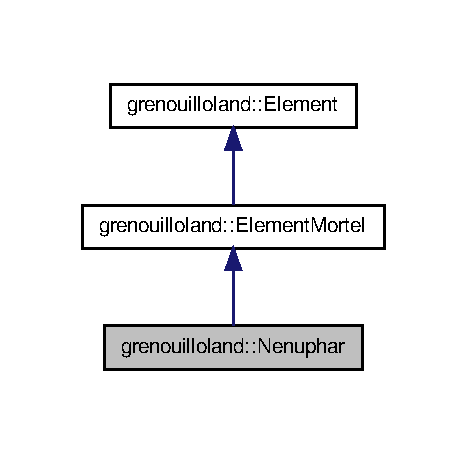
\includegraphics[width=224pt]{classgrenouilloland_1_1Nenuphar__inherit__graph}
\end{center}
\end{figure}


Graphe de collaboration de grenouilloland\-:\-:Nenuphar\-:
\nopagebreak
\begin{figure}[H]
\begin{center}
\leavevmode
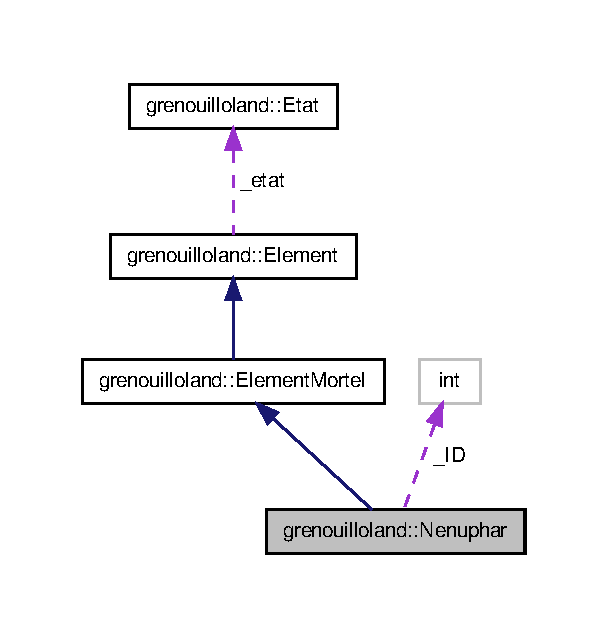
\includegraphics[width=292pt]{classgrenouilloland_1_1Nenuphar__coll__graph}
\end{center}
\end{figure}
\subsection*{Fonctions membres publiques}
\begin{DoxyCompactItemize}
\item 
\hyperlink{classgrenouilloland_1_1Nenuphar_a12e7485c4b6bd9b44f5a835df85bb8bf}{Nenuphar} ()
\item 
\hyperlink{classgrenouilloland_1_1Nenuphar_a0e9471731c8b2763b5ec01e2ad5f20fb}{$\sim$\-Nenuphar} ()
\item 
const int \& \hyperlink{classgrenouilloland_1_1Nenuphar_a3a77c3463dd389cf0eee275ee96a7939}{lire\-Id} () const 
\end{DoxyCompactItemize}
\subsection*{Attributs publics statiques}
\begin{DoxyCompactItemize}
\item 
static const int \hyperlink{classgrenouilloland_1_1Nenuphar_a048ada427d4e142923609003ad468c66}{\-\_\-\-I\-D}
\end{DoxyCompactItemize}
\subsection*{Additional Inherited Members}


\subsection{Description détaillée}
\hyperlink{classgrenouilloland_1_1Nenuphar}{Nenuphar} du \hyperlink{classgrenouilloland_1_1Jeu}{Jeu} Grenouilloland. 

\begin{DoxyAuthor}{Auteur}
Beudin.\-Alexandre Dauxais.\-Yann 
\end{DoxyAuthor}
\begin{DoxyDate}{Date}
05.\-01.\-2012
\end{DoxyDate}
Declaration de la classe \hyperlink{classgrenouilloland_1_1Nenuphar}{Nenuphar} réprésentant un nénuphar classique du jeu Grenouilloland. 

\subsection{Documentation des constructeurs et destructeur}
\hypertarget{classgrenouilloland_1_1Nenuphar_a12e7485c4b6bd9b44f5a835df85bb8bf}{\index{grenouilloland\-::\-Nenuphar@{grenouilloland\-::\-Nenuphar}!Nenuphar@{Nenuphar}}
\index{Nenuphar@{Nenuphar}!grenouilloland::Nenuphar@{grenouilloland\-::\-Nenuphar}}
\subsubsection[{Nenuphar}]{\setlength{\rightskip}{0pt plus 5cm}Nenuphar\-::\-Nenuphar (
\begin{DoxyParamCaption}
{}
\end{DoxyParamCaption}
)}}\label{classgrenouilloland_1_1Nenuphar_a12e7485c4b6bd9b44f5a835df85bb8bf}
Constructeur par défaut du nénuphar. \hypertarget{classgrenouilloland_1_1Nenuphar_a0e9471731c8b2763b5ec01e2ad5f20fb}{\index{grenouilloland\-::\-Nenuphar@{grenouilloland\-::\-Nenuphar}!$\sim$\-Nenuphar@{$\sim$\-Nenuphar}}
\index{$\sim$\-Nenuphar@{$\sim$\-Nenuphar}!grenouilloland::Nenuphar@{grenouilloland\-::\-Nenuphar}}
\subsubsection[{$\sim$\-Nenuphar}]{\setlength{\rightskip}{0pt plus 5cm}Nenuphar\-::$\sim$\-Nenuphar (
\begin{DoxyParamCaption}
{}
\end{DoxyParamCaption}
)}}\label{classgrenouilloland_1_1Nenuphar_a0e9471731c8b2763b5ec01e2ad5f20fb}
Destructeur du nénuphar. 

\subsection{Documentation des fonctions membres}
\hypertarget{classgrenouilloland_1_1Nenuphar_a3a77c3463dd389cf0eee275ee96a7939}{\index{grenouilloland\-::\-Nenuphar@{grenouilloland\-::\-Nenuphar}!lire\-Id@{lire\-Id}}
\index{lire\-Id@{lire\-Id}!grenouilloland::Nenuphar@{grenouilloland\-::\-Nenuphar}}
\subsubsection[{lire\-Id}]{\setlength{\rightskip}{0pt plus 5cm}const int \& Nenuphar\-::lire\-Id (
\begin{DoxyParamCaption}
{}
\end{DoxyParamCaption}
) const\hspace{0.3cm}{\ttfamily [virtual]}}}\label{classgrenouilloland_1_1Nenuphar_a3a77c3463dd389cf0eee275ee96a7939}
Accesseur de l'I\-D identifiant le type nénuphar.

\begin{DoxyReturn}{Renvoie}
la valeur de \hyperlink{classgrenouilloland_1_1Nenuphar_a048ada427d4e142923609003ad468c66}{\-\_\-\-I\-D}.
\end{DoxyReturn}
\begin{DoxyNote}{Note}
L'\-\_\-\-I\-D est const et public mais cet accesseur est nécessaire car il est lu dans la vue sur un objet de type \hyperlink{classgrenouilloland_1_1Element}{Element} et un \hyperlink{classgrenouilloland_1_1Element}{Element} n'a pas d'attribut \-\_\-\-I\-D. 
\end{DoxyNote}


Implémente \hyperlink{classgrenouilloland_1_1Element_aa05b1a2f2e0e8eb0e5ebf942b8934388}{grenouilloland\-::\-Element}.



\subsection{Documentation des données membres}
\hypertarget{classgrenouilloland_1_1Nenuphar_a048ada427d4e142923609003ad468c66}{\index{grenouilloland\-::\-Nenuphar@{grenouilloland\-::\-Nenuphar}!\-\_\-\-I\-D@{\-\_\-\-I\-D}}
\index{\-\_\-\-I\-D@{\-\_\-\-I\-D}!grenouilloland::Nenuphar@{grenouilloland\-::\-Nenuphar}}
\subsubsection[{\-\_\-\-I\-D}]{\setlength{\rightskip}{0pt plus 5cm}const int Nenuphar\-::\-\_\-\-I\-D\hspace{0.3cm}{\ttfamily [static]}}}\label{classgrenouilloland_1_1Nenuphar_a048ada427d4e142923609003ad468c66}
I\-D identifiant le nénuphar. 

La documentation de cette classe a été générée à partir des fichiers suivants \-:\begin{DoxyCompactItemize}
\item 
src/modele/include/Nenuphar.\-hh\item 
src/modele/Nenuphar.\-cpp\end{DoxyCompactItemize}

\hypertarget{classgrenouilloland_1_1NenupharDopant}{\section{Référence de la classe grenouilloland\-:\-:Nenuphar\-Dopant}
\label{classgrenouilloland_1_1NenupharDopant}\index{grenouilloland\-::\-Nenuphar\-Dopant@{grenouilloland\-::\-Nenuphar\-Dopant}}
}


\hyperlink{classgrenouilloland_1_1NenupharDopant}{Nenuphar\-Dopant} du \hyperlink{classgrenouilloland_1_1Jeu}{Jeu} Grenouilloland.  




{\ttfamily \#include $<$Nenuphar\-Dopant.\-hh$>$}



Graphe d'héritage de grenouilloland\-:\-:Nenuphar\-Dopant\-:
\nopagebreak
\begin{figure}[H]
\begin{center}
\leavevmode
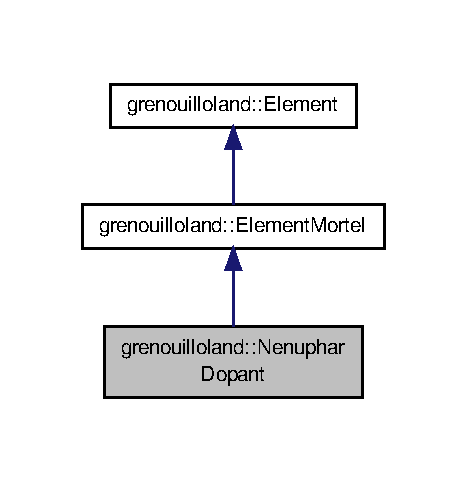
\includegraphics[width=224pt]{classgrenouilloland_1_1NenupharDopant__inherit__graph}
\end{center}
\end{figure}


Graphe de collaboration de grenouilloland\-:\-:Nenuphar\-Dopant\-:
\nopagebreak
\begin{figure}[H]
\begin{center}
\leavevmode
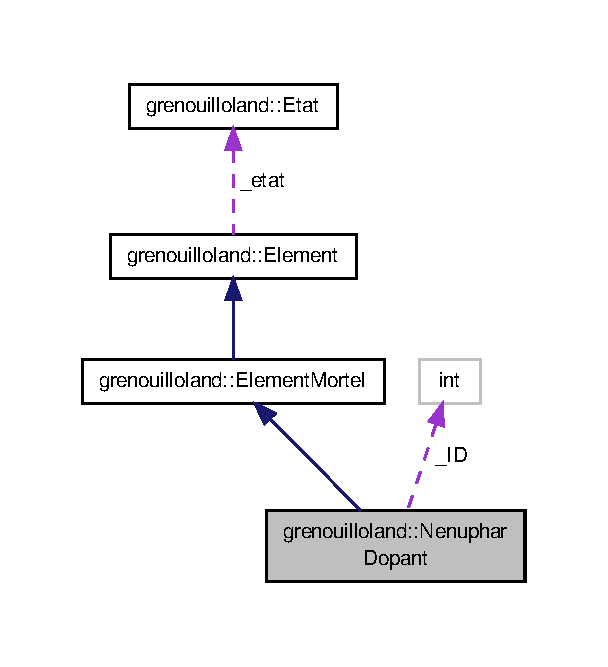
\includegraphics[width=292pt]{classgrenouilloland_1_1NenupharDopant__coll__graph}
\end{center}
\end{figure}
\subsection*{Fonctions membres publiques}
\begin{DoxyCompactItemize}
\item 
\hyperlink{classgrenouilloland_1_1NenupharDopant_af1e5ea1c932d04fe72e6e944a32e52b4}{Nenuphar\-Dopant} ()
\item 
\hyperlink{classgrenouilloland_1_1NenupharDopant_a06781dafde6673932977f636e4c177cd}{$\sim$\-Nenuphar\-Dopant} ()
\item 
const int \& \hyperlink{classgrenouilloland_1_1NenupharDopant_a45374c5e71552f943b8a9729892d5f02}{lire\-Id} () const 
\end{DoxyCompactItemize}
\subsection*{Attributs publics statiques}
\begin{DoxyCompactItemize}
\item 
static const int \hyperlink{classgrenouilloland_1_1NenupharDopant_a4c6cfe51f482da3b7483dde8795787ca}{\-\_\-\-I\-D}
\end{DoxyCompactItemize}
\subsection*{Additional Inherited Members}


\subsection{Description détaillée}
\hyperlink{classgrenouilloland_1_1NenupharDopant}{Nenuphar\-Dopant} du \hyperlink{classgrenouilloland_1_1Jeu}{Jeu} Grenouilloland. 

\begin{DoxyAuthor}{Auteur}
Beudin.\-Alexandre Dauxais.\-Yann 
\end{DoxyAuthor}
\begin{DoxyDate}{Date}
05.\-01.\-2012
\end{DoxyDate}
Declaration de la classe \hyperlink{classgrenouilloland_1_1Nenuphar}{Nenuphar} réprésentant un nénuphar classique du jeu Grenouilloland. 

\subsection{Documentation des constructeurs et destructeur}
\hypertarget{classgrenouilloland_1_1NenupharDopant_af1e5ea1c932d04fe72e6e944a32e52b4}{\index{grenouilloland\-::\-Nenuphar\-Dopant@{grenouilloland\-::\-Nenuphar\-Dopant}!Nenuphar\-Dopant@{Nenuphar\-Dopant}}
\index{Nenuphar\-Dopant@{Nenuphar\-Dopant}!grenouilloland::NenupharDopant@{grenouilloland\-::\-Nenuphar\-Dopant}}
\subsubsection[{Nenuphar\-Dopant}]{\setlength{\rightskip}{0pt plus 5cm}Nenuphar\-Dopant\-::\-Nenuphar\-Dopant (
\begin{DoxyParamCaption}
{}
\end{DoxyParamCaption}
)}}\label{classgrenouilloland_1_1NenupharDopant_af1e5ea1c932d04fe72e6e944a32e52b4}
Constructeur par défaut d'un nénuphar dopant. \hypertarget{classgrenouilloland_1_1NenupharDopant_a06781dafde6673932977f636e4c177cd}{\index{grenouilloland\-::\-Nenuphar\-Dopant@{grenouilloland\-::\-Nenuphar\-Dopant}!$\sim$\-Nenuphar\-Dopant@{$\sim$\-Nenuphar\-Dopant}}
\index{$\sim$\-Nenuphar\-Dopant@{$\sim$\-Nenuphar\-Dopant}!grenouilloland::NenupharDopant@{grenouilloland\-::\-Nenuphar\-Dopant}}
\subsubsection[{$\sim$\-Nenuphar\-Dopant}]{\setlength{\rightskip}{0pt plus 5cm}Nenuphar\-Dopant\-::$\sim$\-Nenuphar\-Dopant (
\begin{DoxyParamCaption}
{}
\end{DoxyParamCaption}
)}}\label{classgrenouilloland_1_1NenupharDopant_a06781dafde6673932977f636e4c177cd}
Destructeur d'un nénuphar dopant. 

\subsection{Documentation des fonctions membres}
\hypertarget{classgrenouilloland_1_1NenupharDopant_a45374c5e71552f943b8a9729892d5f02}{\index{grenouilloland\-::\-Nenuphar\-Dopant@{grenouilloland\-::\-Nenuphar\-Dopant}!lire\-Id@{lire\-Id}}
\index{lire\-Id@{lire\-Id}!grenouilloland::NenupharDopant@{grenouilloland\-::\-Nenuphar\-Dopant}}
\subsubsection[{lire\-Id}]{\setlength{\rightskip}{0pt plus 5cm}const int \& Nenuphar\-Dopant\-::lire\-Id (
\begin{DoxyParamCaption}
{}
\end{DoxyParamCaption}
) const\hspace{0.3cm}{\ttfamily [virtual]}}}\label{classgrenouilloland_1_1NenupharDopant_a45374c5e71552f943b8a9729892d5f02}
Acceseur à l'I\-D définissant un nénupahr dopant.

\begin{DoxyReturn}{Renvoie}
la valeur de \hyperlink{classgrenouilloland_1_1NenupharDopant_a4c6cfe51f482da3b7483dde8795787ca}{\-\_\-\-I\-D}.
\end{DoxyReturn}
\begin{DoxyNote}{Note}
L'\-\_\-\-I\-D est const et public mais cet accesseur est nécessaire car il est lu dans la vue sur un objet de type \hyperlink{classgrenouilloland_1_1Element}{Element} et un \hyperlink{classgrenouilloland_1_1Element}{Element} n'a pas d'attribut \-\_\-\-I\-D. 
\end{DoxyNote}


Implémente \hyperlink{classgrenouilloland_1_1Element_aa05b1a2f2e0e8eb0e5ebf942b8934388}{grenouilloland\-::\-Element}.



\subsection{Documentation des données membres}
\hypertarget{classgrenouilloland_1_1NenupharDopant_a4c6cfe51f482da3b7483dde8795787ca}{\index{grenouilloland\-::\-Nenuphar\-Dopant@{grenouilloland\-::\-Nenuphar\-Dopant}!\-\_\-\-I\-D@{\-\_\-\-I\-D}}
\index{\-\_\-\-I\-D@{\-\_\-\-I\-D}!grenouilloland::NenupharDopant@{grenouilloland\-::\-Nenuphar\-Dopant}}
\subsubsection[{\-\_\-\-I\-D}]{\setlength{\rightskip}{0pt plus 5cm}const int Nenuphar\-Dopant\-::\-\_\-\-I\-D\hspace{0.3cm}{\ttfamily [static]}}}\label{classgrenouilloland_1_1NenupharDopant_a4c6cfe51f482da3b7483dde8795787ca}
I\-D définissant un nénuphar dopant. 

La documentation de cette classe a été générée à partir des fichiers suivants \-:\begin{DoxyCompactItemize}
\item 
src/modele/include/Nenuphar\-Dopant.\-hh\item 
src/modele/Nenuphar\-Dopant.\-cpp\end{DoxyCompactItemize}

\hypertarget{classgrenouilloland_1_1NenupharImmortel}{\section{Référence de la classe grenouilloland\-:\-:Nenuphar\-Immortel}
\label{classgrenouilloland_1_1NenupharImmortel}\index{grenouilloland\-::\-Nenuphar\-Immortel@{grenouilloland\-::\-Nenuphar\-Immortel}}
}


\hyperlink{classgrenouilloland_1_1NenupharImmortel}{Nenuphar\-Immortel} du \hyperlink{classgrenouilloland_1_1Jeu}{Jeu} Grenouilloland.  




{\ttfamily \#include $<$Nenuphar\-Immortel.\-hh$>$}



Graphe d'héritage de grenouilloland\-:\-:Nenuphar\-Immortel\-:
\nopagebreak
\begin{figure}[H]
\begin{center}
\leavevmode
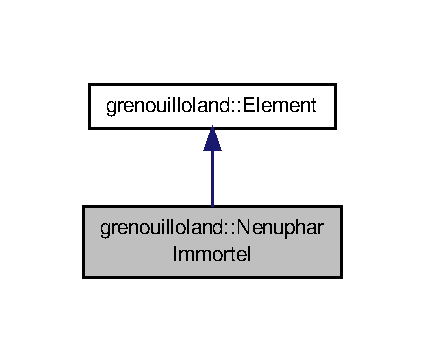
\includegraphics[width=204pt]{classgrenouilloland_1_1NenupharImmortel__inherit__graph}
\end{center}
\end{figure}


Graphe de collaboration de grenouilloland\-:\-:Nenuphar\-Immortel\-:
\nopagebreak
\begin{figure}[H]
\begin{center}
\leavevmode
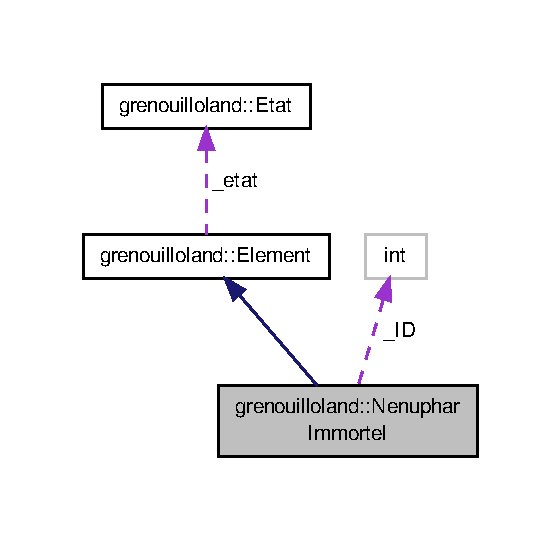
\includegraphics[width=269pt]{classgrenouilloland_1_1NenupharImmortel__coll__graph}
\end{center}
\end{figure}
\subsection*{Fonctions membres publiques}
\begin{DoxyCompactItemize}
\item 
\hyperlink{classgrenouilloland_1_1NenupharImmortel_aa4dd57433beb66c620a5a413bf4ffd49}{Nenuphar\-Immortel} ()
\item 
\hyperlink{classgrenouilloland_1_1NenupharImmortel_a23898629dbe543bfa8e69278389fc7b4}{$\sim$\-Nenuphar\-Immortel} ()
\item 
const int \& \hyperlink{classgrenouilloland_1_1NenupharImmortel_a6fadef66c4d46dea30e0b5ba933ff1d6}{lire\-Id} () const 
\end{DoxyCompactItemize}
\subsection*{Attributs publics statiques}
\begin{DoxyCompactItemize}
\item 
static const int \hyperlink{classgrenouilloland_1_1NenupharImmortel_a1a37a7af6e1296d47556752041b2fe18}{\-\_\-\-I\-D}
\end{DoxyCompactItemize}
\subsection*{Additional Inherited Members}


\subsection{Description détaillée}
\hyperlink{classgrenouilloland_1_1NenupharImmortel}{Nenuphar\-Immortel} du \hyperlink{classgrenouilloland_1_1Jeu}{Jeu} Grenouilloland. 

\begin{DoxyAuthor}{Auteur}
Beudin.\-Alexandre Dauxais.\-Yann 
\end{DoxyAuthor}
\begin{DoxyDate}{Date}
05.\-01.\-2012
\end{DoxyDate}
Declaration de la classe \hyperlink{classgrenouilloland_1_1NenupharImmortel}{Nenuphar\-Immortel} réprésentant un nénuphar immortel du jeu Grenouilloland. 

\subsection{Documentation des constructeurs et destructeur}
\hypertarget{classgrenouilloland_1_1NenupharImmortel_aa4dd57433beb66c620a5a413bf4ffd49}{\index{grenouilloland\-::\-Nenuphar\-Immortel@{grenouilloland\-::\-Nenuphar\-Immortel}!Nenuphar\-Immortel@{Nenuphar\-Immortel}}
\index{Nenuphar\-Immortel@{Nenuphar\-Immortel}!grenouilloland::NenupharImmortel@{grenouilloland\-::\-Nenuphar\-Immortel}}
\subsubsection[{Nenuphar\-Immortel}]{\setlength{\rightskip}{0pt plus 5cm}Nenuphar\-Immortel\-::\-Nenuphar\-Immortel (
\begin{DoxyParamCaption}
{}
\end{DoxyParamCaption}
)}}\label{classgrenouilloland_1_1NenupharImmortel_aa4dd57433beb66c620a5a413bf4ffd49}
Constructeur par défaut d'un nénuphar immortel. \hypertarget{classgrenouilloland_1_1NenupharImmortel_a23898629dbe543bfa8e69278389fc7b4}{\index{grenouilloland\-::\-Nenuphar\-Immortel@{grenouilloland\-::\-Nenuphar\-Immortel}!$\sim$\-Nenuphar\-Immortel@{$\sim$\-Nenuphar\-Immortel}}
\index{$\sim$\-Nenuphar\-Immortel@{$\sim$\-Nenuphar\-Immortel}!grenouilloland::NenupharImmortel@{grenouilloland\-::\-Nenuphar\-Immortel}}
\subsubsection[{$\sim$\-Nenuphar\-Immortel}]{\setlength{\rightskip}{0pt plus 5cm}Nenuphar\-Immortel\-::$\sim$\-Nenuphar\-Immortel (
\begin{DoxyParamCaption}
{}
\end{DoxyParamCaption}
)}}\label{classgrenouilloland_1_1NenupharImmortel_a23898629dbe543bfa8e69278389fc7b4}
Destructeur d'un nénuphar immortel. 

\subsection{Documentation des fonctions membres}
\hypertarget{classgrenouilloland_1_1NenupharImmortel_a6fadef66c4d46dea30e0b5ba933ff1d6}{\index{grenouilloland\-::\-Nenuphar\-Immortel@{grenouilloland\-::\-Nenuphar\-Immortel}!lire\-Id@{lire\-Id}}
\index{lire\-Id@{lire\-Id}!grenouilloland::NenupharImmortel@{grenouilloland\-::\-Nenuphar\-Immortel}}
\subsubsection[{lire\-Id}]{\setlength{\rightskip}{0pt plus 5cm}const int \& Nenuphar\-Immortel\-::lire\-Id (
\begin{DoxyParamCaption}
{}
\end{DoxyParamCaption}
) const\hspace{0.3cm}{\ttfamily [virtual]}}}\label{classgrenouilloland_1_1NenupharImmortel_a6fadef66c4d46dea30e0b5ba933ff1d6}
Accesseur de l'I\-D identifiant un nénuphar immortel.

\begin{DoxyReturn}{Renvoie}
la valeur de \hyperlink{classgrenouilloland_1_1NenupharImmortel_a1a37a7af6e1296d47556752041b2fe18}{\-\_\-\-I\-D}.
\end{DoxyReturn}
\begin{DoxyNote}{Note}
L'\-\_\-\-I\-D est const et public mais cet accesseur est nécessaire car il est lu dans la vue sur un objet de type \hyperlink{classgrenouilloland_1_1Element}{Element} et un \hyperlink{classgrenouilloland_1_1Element}{Element} n'a pas d'attribut \-\_\-\-I\-D. 
\end{DoxyNote}


Implémente \hyperlink{classgrenouilloland_1_1Element_aa05b1a2f2e0e8eb0e5ebf942b8934388}{grenouilloland\-::\-Element}.



\subsection{Documentation des données membres}
\hypertarget{classgrenouilloland_1_1NenupharImmortel_a1a37a7af6e1296d47556752041b2fe18}{\index{grenouilloland\-::\-Nenuphar\-Immortel@{grenouilloland\-::\-Nenuphar\-Immortel}!\-\_\-\-I\-D@{\-\_\-\-I\-D}}
\index{\-\_\-\-I\-D@{\-\_\-\-I\-D}!grenouilloland::NenupharImmortel@{grenouilloland\-::\-Nenuphar\-Immortel}}
\subsubsection[{\-\_\-\-I\-D}]{\setlength{\rightskip}{0pt plus 5cm}const int Nenuphar\-Immortel\-::\-\_\-\-I\-D\hspace{0.3cm}{\ttfamily [static]}}}\label{classgrenouilloland_1_1NenupharImmortel_a1a37a7af6e1296d47556752041b2fe18}
I\-D définissant un nénuphar immortel. 

La documentation de cette classe a été générée à partir des fichiers suivants \-:\begin{DoxyCompactItemize}
\item 
src/modele/include/Nenuphar\-Immortel.\-hh\item 
src/modele/Nenuphar\-Immortel.\-cpp\end{DoxyCompactItemize}

\hypertarget{classgrenouilloland_1_1NenupharMortel}{\section{Référence de la classe grenouilloland\-:\-:Nenuphar\-Mortel}
\label{classgrenouilloland_1_1NenupharMortel}\index{grenouilloland\-::\-Nenuphar\-Mortel@{grenouilloland\-::\-Nenuphar\-Mortel}}
}


\hyperlink{classgrenouilloland_1_1NenupharMortel}{Nenuphar\-Mortel} du \hyperlink{classgrenouilloland_1_1Jeu}{Jeu} Grenouilloland.  




{\ttfamily \#include $<$Nenuphar\-Mortel.\-hh$>$}



Graphe d'héritage de grenouilloland\-:\-:Nenuphar\-Mortel\-:
\nopagebreak
\begin{figure}[H]
\begin{center}
\leavevmode
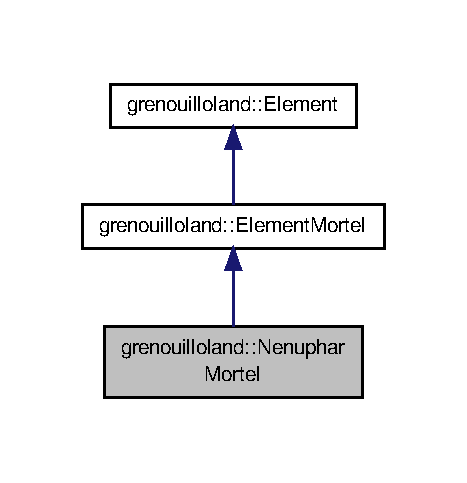
\includegraphics[width=224pt]{classgrenouilloland_1_1NenupharMortel__inherit__graph}
\end{center}
\end{figure}


Graphe de collaboration de grenouilloland\-:\-:Nenuphar\-Mortel\-:
\nopagebreak
\begin{figure}[H]
\begin{center}
\leavevmode
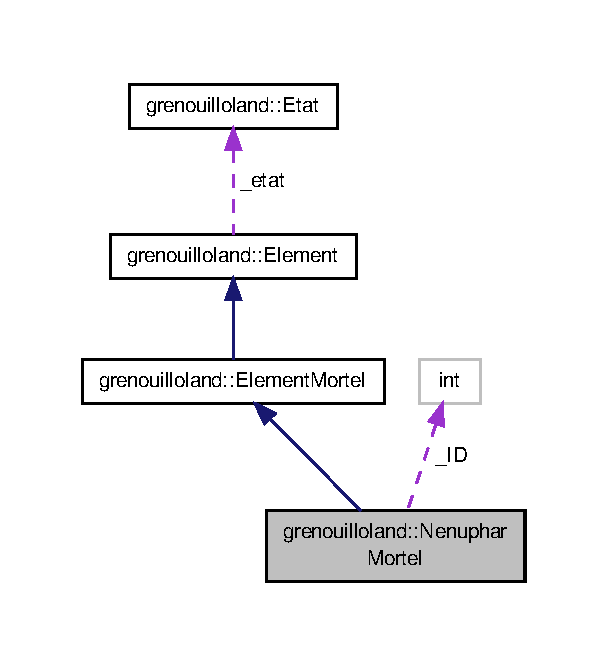
\includegraphics[width=292pt]{classgrenouilloland_1_1NenupharMortel__coll__graph}
\end{center}
\end{figure}
\subsection*{Fonctions membres publiques}
\begin{DoxyCompactItemize}
\item 
\hyperlink{classgrenouilloland_1_1NenupharMortel_a6e130520aa36b6d049a0db7198da113e}{Nenuphar\-Mortel} ()
\item 
\hyperlink{classgrenouilloland_1_1NenupharMortel_a870864bde15f443491e66e463a73e525}{$\sim$\-Nenuphar\-Mortel} ()
\item 
const int \& \hyperlink{classgrenouilloland_1_1NenupharMortel_aac1c7add92c76c06a2848fe264a59bdd}{lire\-Id} () const 
\end{DoxyCompactItemize}
\subsection*{Attributs publics statiques}
\begin{DoxyCompactItemize}
\item 
static const int \hyperlink{classgrenouilloland_1_1NenupharMortel_aa64713741f9e0f83140b831dcab0f67f}{\-\_\-\-I\-D}
\end{DoxyCompactItemize}
\subsection*{Additional Inherited Members}


\subsection{Description détaillée}
\hyperlink{classgrenouilloland_1_1NenupharMortel}{Nenuphar\-Mortel} du \hyperlink{classgrenouilloland_1_1Jeu}{Jeu} Grenouilloland. 

\begin{DoxyAuthor}{Auteur}
Beudin.\-Alexandre Dauxais.\-Yann 
\end{DoxyAuthor}
\begin{DoxyDate}{Date}
05.\-01.\-2012
\end{DoxyDate}
Declaration de la classe \hyperlink{classgrenouilloland_1_1NenupharMortel}{Nenuphar\-Mortel} réprésentant un nénuphar mortel du jeu Grenouilloland. 

\subsection{Documentation des constructeurs et destructeur}
\hypertarget{classgrenouilloland_1_1NenupharMortel_a6e130520aa36b6d049a0db7198da113e}{\index{grenouilloland\-::\-Nenuphar\-Mortel@{grenouilloland\-::\-Nenuphar\-Mortel}!Nenuphar\-Mortel@{Nenuphar\-Mortel}}
\index{Nenuphar\-Mortel@{Nenuphar\-Mortel}!grenouilloland::NenupharMortel@{grenouilloland\-::\-Nenuphar\-Mortel}}
\subsubsection[{Nenuphar\-Mortel}]{\setlength{\rightskip}{0pt plus 5cm}Nenuphar\-Mortel\-::\-Nenuphar\-Mortel (
\begin{DoxyParamCaption}
{}
\end{DoxyParamCaption}
)}}\label{classgrenouilloland_1_1NenupharMortel_a6e130520aa36b6d049a0db7198da113e}
Constructeur par défaut d'un nénuphar mortel. \hypertarget{classgrenouilloland_1_1NenupharMortel_a870864bde15f443491e66e463a73e525}{\index{grenouilloland\-::\-Nenuphar\-Mortel@{grenouilloland\-::\-Nenuphar\-Mortel}!$\sim$\-Nenuphar\-Mortel@{$\sim$\-Nenuphar\-Mortel}}
\index{$\sim$\-Nenuphar\-Mortel@{$\sim$\-Nenuphar\-Mortel}!grenouilloland::NenupharMortel@{grenouilloland\-::\-Nenuphar\-Mortel}}
\subsubsection[{$\sim$\-Nenuphar\-Mortel}]{\setlength{\rightskip}{0pt plus 5cm}Nenuphar\-Mortel\-::$\sim$\-Nenuphar\-Mortel (
\begin{DoxyParamCaption}
{}
\end{DoxyParamCaption}
)}}\label{classgrenouilloland_1_1NenupharMortel_a870864bde15f443491e66e463a73e525}
Destructeur d'un nénuphar mortel. 

\subsection{Documentation des fonctions membres}
\hypertarget{classgrenouilloland_1_1NenupharMortel_aac1c7add92c76c06a2848fe264a59bdd}{\index{grenouilloland\-::\-Nenuphar\-Mortel@{grenouilloland\-::\-Nenuphar\-Mortel}!lire\-Id@{lire\-Id}}
\index{lire\-Id@{lire\-Id}!grenouilloland::NenupharMortel@{grenouilloland\-::\-Nenuphar\-Mortel}}
\subsubsection[{lire\-Id}]{\setlength{\rightskip}{0pt plus 5cm}const int \& Nenuphar\-Mortel\-::lire\-Id (
\begin{DoxyParamCaption}
{}
\end{DoxyParamCaption}
) const\hspace{0.3cm}{\ttfamily [virtual]}}}\label{classgrenouilloland_1_1NenupharMortel_aac1c7add92c76c06a2848fe264a59bdd}
Accesseur de l'I\-D identifiant un nénuphar mortel.

\begin{DoxyReturn}{Renvoie}
la valeur de \hyperlink{classgrenouilloland_1_1NenupharMortel_aa64713741f9e0f83140b831dcab0f67f}{\-\_\-\-I\-D}.
\end{DoxyReturn}
\begin{DoxyNote}{Note}
L'\-\_\-\-I\-D est const et public mais cet accesseur est nécessaire car il est lu dans la vue sur un objet de type \hyperlink{classgrenouilloland_1_1Element}{Element} et un \hyperlink{classgrenouilloland_1_1Element}{Element} n'a pas d'attribut \-\_\-\-I\-D. 
\end{DoxyNote}


Implémente \hyperlink{classgrenouilloland_1_1Element_aa05b1a2f2e0e8eb0e5ebf942b8934388}{grenouilloland\-::\-Element}.



\subsection{Documentation des données membres}
\hypertarget{classgrenouilloland_1_1NenupharMortel_aa64713741f9e0f83140b831dcab0f67f}{\index{grenouilloland\-::\-Nenuphar\-Mortel@{grenouilloland\-::\-Nenuphar\-Mortel}!\-\_\-\-I\-D@{\-\_\-\-I\-D}}
\index{\-\_\-\-I\-D@{\-\_\-\-I\-D}!grenouilloland::NenupharMortel@{grenouilloland\-::\-Nenuphar\-Mortel}}
\subsubsection[{\-\_\-\-I\-D}]{\setlength{\rightskip}{0pt plus 5cm}const int Nenuphar\-Mortel\-::\-\_\-\-I\-D\hspace{0.3cm}{\ttfamily [static]}}}\label{classgrenouilloland_1_1NenupharMortel_aa64713741f9e0f83140b831dcab0f67f}
I\-D identifiant un nénuphar mortel. 

La documentation de cette classe a été générée à partir des fichiers suivants \-:\begin{DoxyCompactItemize}
\item 
src/modele/include/Nenuphar\-Mortel.\-hh\item 
src/modele/Nenuphar\-Mortel.\-cpp\end{DoxyCompactItemize}

\hypertarget{classgrenouilloland_1_1NenupharNutritif}{\section{Référence de la classe grenouilloland\-:\-:Nenuphar\-Nutritif}
\label{classgrenouilloland_1_1NenupharNutritif}\index{grenouilloland\-::\-Nenuphar\-Nutritif@{grenouilloland\-::\-Nenuphar\-Nutritif}}
}


\hyperlink{classgrenouilloland_1_1NenupharNutritif}{Nenuphar\-Nutritif} du \hyperlink{classgrenouilloland_1_1Jeu}{Jeu} Grenouilloland.  




{\ttfamily \#include $<$Nenuphar\-Nutritif.\-hh$>$}



Graphe d'héritage de grenouilloland\-:\-:Nenuphar\-Nutritif\-:
\nopagebreak
\begin{figure}[H]
\begin{center}
\leavevmode
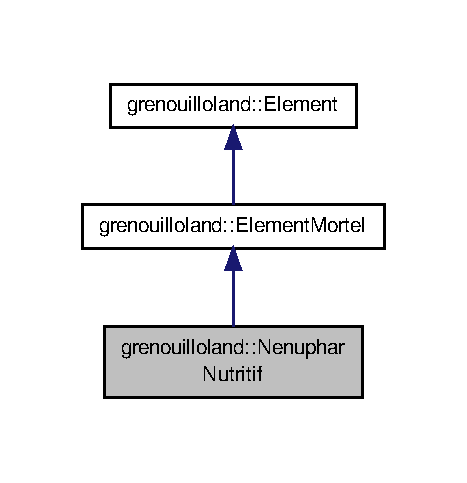
\includegraphics[width=224pt]{classgrenouilloland_1_1NenupharNutritif__inherit__graph}
\end{center}
\end{figure}


Graphe de collaboration de grenouilloland\-:\-:Nenuphar\-Nutritif\-:
\nopagebreak
\begin{figure}[H]
\begin{center}
\leavevmode
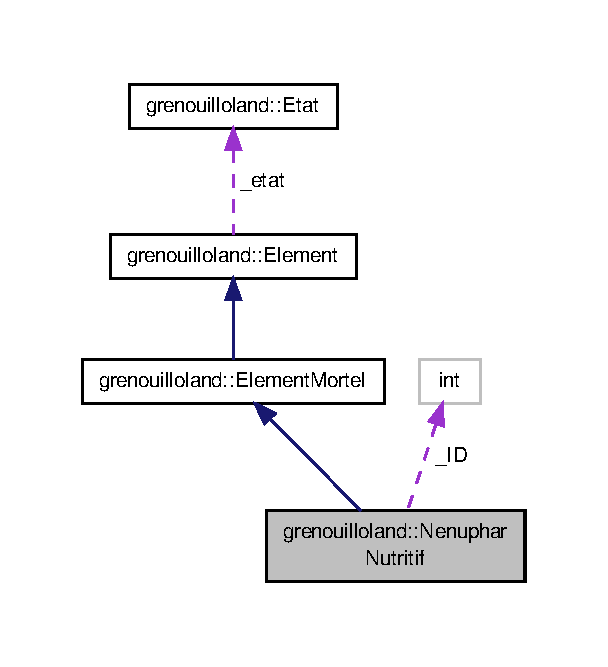
\includegraphics[width=292pt]{classgrenouilloland_1_1NenupharNutritif__coll__graph}
\end{center}
\end{figure}
\subsection*{Fonctions membres publiques}
\begin{DoxyCompactItemize}
\item 
\hyperlink{classgrenouilloland_1_1NenupharNutritif_aedd08b77d494dab677136bd8fef1fb98}{Nenuphar\-Nutritif} ()
\item 
\hyperlink{classgrenouilloland_1_1NenupharNutritif_a6a2cbb69872e858c9786dfeac0351f10}{$\sim$\-Nenuphar\-Nutritif} ()
\item 
const int \& \hyperlink{classgrenouilloland_1_1NenupharNutritif_ac27d0cfbf8e2f4ee647031983a5fc1f4}{lire\-Id} () const 
\end{DoxyCompactItemize}
\subsection*{Attributs publics statiques}
\begin{DoxyCompactItemize}
\item 
static const int \hyperlink{classgrenouilloland_1_1NenupharNutritif_acfbcd62da4052d83f2b11e1a6baabe8d}{\-\_\-\-I\-D}
\end{DoxyCompactItemize}
\subsection*{Additional Inherited Members}


\subsection{Description détaillée}
\hyperlink{classgrenouilloland_1_1NenupharNutritif}{Nenuphar\-Nutritif} du \hyperlink{classgrenouilloland_1_1Jeu}{Jeu} Grenouilloland. 

\begin{DoxyAuthor}{Auteur}
Beudin.\-Alexandre Dauxais.\-Yann 
\end{DoxyAuthor}
\begin{DoxyDate}{Date}
05.\-01.\-2012
\end{DoxyDate}
Declaration de la classe \hyperlink{classgrenouilloland_1_1NenupharNutritif}{Nenuphar\-Nutritif} réprésentant un nénuphar nutritif du jeu Grenouilloland. 

\subsection{Documentation des constructeurs et destructeur}
\hypertarget{classgrenouilloland_1_1NenupharNutritif_aedd08b77d494dab677136bd8fef1fb98}{\index{grenouilloland\-::\-Nenuphar\-Nutritif@{grenouilloland\-::\-Nenuphar\-Nutritif}!Nenuphar\-Nutritif@{Nenuphar\-Nutritif}}
\index{Nenuphar\-Nutritif@{Nenuphar\-Nutritif}!grenouilloland::NenupharNutritif@{grenouilloland\-::\-Nenuphar\-Nutritif}}
\subsubsection[{Nenuphar\-Nutritif}]{\setlength{\rightskip}{0pt plus 5cm}Nenuphar\-Nutritif\-::\-Nenuphar\-Nutritif (
\begin{DoxyParamCaption}
{}
\end{DoxyParamCaption}
)}}\label{classgrenouilloland_1_1NenupharNutritif_aedd08b77d494dab677136bd8fef1fb98}
Constructeur par défaut d'un nénuphar nutritif. \hypertarget{classgrenouilloland_1_1NenupharNutritif_a6a2cbb69872e858c9786dfeac0351f10}{\index{grenouilloland\-::\-Nenuphar\-Nutritif@{grenouilloland\-::\-Nenuphar\-Nutritif}!$\sim$\-Nenuphar\-Nutritif@{$\sim$\-Nenuphar\-Nutritif}}
\index{$\sim$\-Nenuphar\-Nutritif@{$\sim$\-Nenuphar\-Nutritif}!grenouilloland::NenupharNutritif@{grenouilloland\-::\-Nenuphar\-Nutritif}}
\subsubsection[{$\sim$\-Nenuphar\-Nutritif}]{\setlength{\rightskip}{0pt plus 5cm}Nenuphar\-Nutritif\-::$\sim$\-Nenuphar\-Nutritif (
\begin{DoxyParamCaption}
{}
\end{DoxyParamCaption}
)}}\label{classgrenouilloland_1_1NenupharNutritif_a6a2cbb69872e858c9786dfeac0351f10}
Destructeur d'un nénuphar nutritif. 

\subsection{Documentation des fonctions membres}
\hypertarget{classgrenouilloland_1_1NenupharNutritif_ac27d0cfbf8e2f4ee647031983a5fc1f4}{\index{grenouilloland\-::\-Nenuphar\-Nutritif@{grenouilloland\-::\-Nenuphar\-Nutritif}!lire\-Id@{lire\-Id}}
\index{lire\-Id@{lire\-Id}!grenouilloland::NenupharNutritif@{grenouilloland\-::\-Nenuphar\-Nutritif}}
\subsubsection[{lire\-Id}]{\setlength{\rightskip}{0pt plus 5cm}const int \& Nenuphar\-Nutritif\-::lire\-Id (
\begin{DoxyParamCaption}
{}
\end{DoxyParamCaption}
) const\hspace{0.3cm}{\ttfamily [virtual]}}}\label{classgrenouilloland_1_1NenupharNutritif_ac27d0cfbf8e2f4ee647031983a5fc1f4}
Accesseur de l'I\-D identifiant un nénuphar nutritif.

\begin{DoxyReturn}{Renvoie}
la valeur de \hyperlink{classgrenouilloland_1_1NenupharNutritif_acfbcd62da4052d83f2b11e1a6baabe8d}{\-\_\-\-I\-D}.
\end{DoxyReturn}
\begin{DoxyNote}{Note}
L'\-\_\-\-I\-D est const et public mais cet accesseur est nécessaire car il est lu dans la vue sur un objet de type \hyperlink{classgrenouilloland_1_1Element}{Element} et un \hyperlink{classgrenouilloland_1_1Element}{Element} n'a pas d'attribut \-\_\-\-I\-D. 
\end{DoxyNote}


Implémente \hyperlink{classgrenouilloland_1_1Element_aa05b1a2f2e0e8eb0e5ebf942b8934388}{grenouilloland\-::\-Element}.



\subsection{Documentation des données membres}
\hypertarget{classgrenouilloland_1_1NenupharNutritif_acfbcd62da4052d83f2b11e1a6baabe8d}{\index{grenouilloland\-::\-Nenuphar\-Nutritif@{grenouilloland\-::\-Nenuphar\-Nutritif}!\-\_\-\-I\-D@{\-\_\-\-I\-D}}
\index{\-\_\-\-I\-D@{\-\_\-\-I\-D}!grenouilloland::NenupharNutritif@{grenouilloland\-::\-Nenuphar\-Nutritif}}
\subsubsection[{\-\_\-\-I\-D}]{\setlength{\rightskip}{0pt plus 5cm}const int Nenuphar\-Nutritif\-::\-\_\-\-I\-D\hspace{0.3cm}{\ttfamily [static]}}}\label{classgrenouilloland_1_1NenupharNutritif_acfbcd62da4052d83f2b11e1a6baabe8d}
I\-D identifiant un nénuphar nutritif. 

La documentation de cette classe a été générée à partir des fichiers suivants \-:\begin{DoxyCompactItemize}
\item 
src/modele/include/Nenuphar\-Nutritif.\-hh\item 
src/modele/Nenuphar\-Nutritif.\-cpp\end{DoxyCompactItemize}

\hypertarget{classgrenouilloland_1_1NenupharVeneneux}{\section{Référence de la classe grenouilloland\-:\-:Nenuphar\-Veneneux}
\label{classgrenouilloland_1_1NenupharVeneneux}\index{grenouilloland\-::\-Nenuphar\-Veneneux@{grenouilloland\-::\-Nenuphar\-Veneneux}}
}


\hyperlink{classgrenouilloland_1_1NenupharVeneneux}{Nenuphar\-Veneneux} du \hyperlink{classgrenouilloland_1_1Jeu}{Jeu} Grenouilloland.  




{\ttfamily \#include $<$Nenuphar\-Veneneux.\-hh$>$}



Graphe d'héritage de grenouilloland\-:\-:Nenuphar\-Veneneux\-:
\nopagebreak
\begin{figure}[H]
\begin{center}
\leavevmode
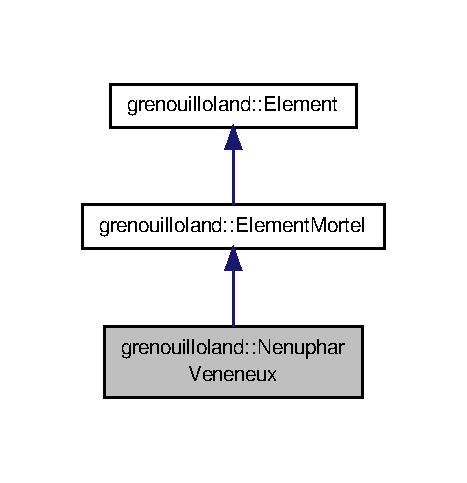
\includegraphics[width=224pt]{classgrenouilloland_1_1NenupharVeneneux__inherit__graph}
\end{center}
\end{figure}


Graphe de collaboration de grenouilloland\-:\-:Nenuphar\-Veneneux\-:
\nopagebreak
\begin{figure}[H]
\begin{center}
\leavevmode
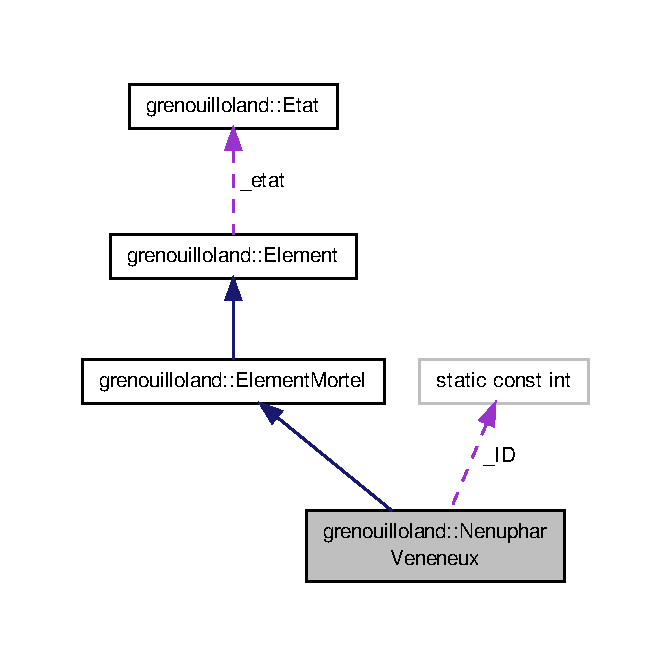
\includegraphics[width=322pt]{classgrenouilloland_1_1NenupharVeneneux__coll__graph}
\end{center}
\end{figure}
\subsection*{Fonctions membres publiques}
\begin{DoxyCompactItemize}
\item 
\hyperlink{classgrenouilloland_1_1NenupharVeneneux_a32998a823da3d578faab3eda91cee837}{Nenuphar\-Veneneux} ()
\item 
\hyperlink{classgrenouilloland_1_1NenupharVeneneux_a350f1d66b75499dd18a7adf455d9e680}{$\sim$\-Nenuphar\-Veneneux} ()
\item 
const int \& \hyperlink{classgrenouilloland_1_1NenupharVeneneux_afbf5c6a0b2f88d65027a6582dca402d1}{lire\-Id} () const 
\end{DoxyCompactItemize}
\subsection*{Attributs publics statiques}
\begin{DoxyCompactItemize}
\item 
static const int \hyperlink{classgrenouilloland_1_1NenupharVeneneux_a2cfb9132dd85224aae2b01e769133d22}{\-\_\-\-I\-D}
\end{DoxyCompactItemize}
\subsection*{Additional Inherited Members}


\subsection{Description détaillée}
\hyperlink{classgrenouilloland_1_1NenupharVeneneux}{Nenuphar\-Veneneux} du \hyperlink{classgrenouilloland_1_1Jeu}{Jeu} Grenouilloland. 

\begin{DoxyAuthor}{Auteur}
Beudin.\-Alexandre Dauxais.\-Yann 
\end{DoxyAuthor}
\begin{DoxyDate}{Date}
05.\-01.\-2012
\end{DoxyDate}
Declaration de la classe \hyperlink{classgrenouilloland_1_1NenupharVeneneux}{Nenuphar\-Veneneux} réprésentant un nénuphar vénéneux du jeu Grenouilloland. 

\subsection{Documentation des constructeurs et destructeur}
\hypertarget{classgrenouilloland_1_1NenupharVeneneux_a32998a823da3d578faab3eda91cee837}{\index{grenouilloland\-::\-Nenuphar\-Veneneux@{grenouilloland\-::\-Nenuphar\-Veneneux}!Nenuphar\-Veneneux@{Nenuphar\-Veneneux}}
\index{Nenuphar\-Veneneux@{Nenuphar\-Veneneux}!grenouilloland::NenupharVeneneux@{grenouilloland\-::\-Nenuphar\-Veneneux}}
\subsubsection[{Nenuphar\-Veneneux}]{\setlength{\rightskip}{0pt plus 5cm}Nenuphar\-Veneneux\-::\-Nenuphar\-Veneneux (
\begin{DoxyParamCaption}
{}
\end{DoxyParamCaption}
)}}\label{classgrenouilloland_1_1NenupharVeneneux_a32998a823da3d578faab3eda91cee837}
Constructeur par défaut d'un nénuphar vénéneux. \hypertarget{classgrenouilloland_1_1NenupharVeneneux_a350f1d66b75499dd18a7adf455d9e680}{\index{grenouilloland\-::\-Nenuphar\-Veneneux@{grenouilloland\-::\-Nenuphar\-Veneneux}!$\sim$\-Nenuphar\-Veneneux@{$\sim$\-Nenuphar\-Veneneux}}
\index{$\sim$\-Nenuphar\-Veneneux@{$\sim$\-Nenuphar\-Veneneux}!grenouilloland::NenupharVeneneux@{grenouilloland\-::\-Nenuphar\-Veneneux}}
\subsubsection[{$\sim$\-Nenuphar\-Veneneux}]{\setlength{\rightskip}{0pt plus 5cm}Nenuphar\-Veneneux\-::$\sim$\-Nenuphar\-Veneneux (
\begin{DoxyParamCaption}
{}
\end{DoxyParamCaption}
)}}\label{classgrenouilloland_1_1NenupharVeneneux_a350f1d66b75499dd18a7adf455d9e680}
Destructeur d'un nénuphar vénéneux. 

\subsection{Documentation des fonctions membres}
\hypertarget{classgrenouilloland_1_1NenupharVeneneux_afbf5c6a0b2f88d65027a6582dca402d1}{\index{grenouilloland\-::\-Nenuphar\-Veneneux@{grenouilloland\-::\-Nenuphar\-Veneneux}!lire\-Id@{lire\-Id}}
\index{lire\-Id@{lire\-Id}!grenouilloland::NenupharVeneneux@{grenouilloland\-::\-Nenuphar\-Veneneux}}
\subsubsection[{lire\-Id}]{\setlength{\rightskip}{0pt plus 5cm}const int \& Nenuphar\-Veneneux\-::lire\-Id (
\begin{DoxyParamCaption}
{}
\end{DoxyParamCaption}
) const\hspace{0.3cm}{\ttfamily [virtual]}}}\label{classgrenouilloland_1_1NenupharVeneneux_afbf5c6a0b2f88d65027a6582dca402d1}
Accesseur de l'I\-D identifiant un nénuphar vénéneux.

\begin{DoxyReturn}{Renvoie}
la valeur de \hyperlink{classgrenouilloland_1_1NenupharVeneneux_a2cfb9132dd85224aae2b01e769133d22}{\-\_\-\-I\-D}.
\end{DoxyReturn}
\begin{DoxyNote}{Note}
L'\-\_\-\-I\-D est const et public mais cet accesseur est nécessaire car il est lu dans la vue sur un objet de type \hyperlink{classgrenouilloland_1_1Element}{Element} et un \hyperlink{classgrenouilloland_1_1Element}{Element} n'a pas d'attribut \-\_\-\-I\-D. 
\end{DoxyNote}


Implémente \hyperlink{classgrenouilloland_1_1Element_aa05b1a2f2e0e8eb0e5ebf942b8934388}{grenouilloland\-::\-Element}.



\subsection{Documentation des données membres}
\hypertarget{classgrenouilloland_1_1NenupharVeneneux_a2cfb9132dd85224aae2b01e769133d22}{\index{grenouilloland\-::\-Nenuphar\-Veneneux@{grenouilloland\-::\-Nenuphar\-Veneneux}!\-\_\-\-I\-D@{\-\_\-\-I\-D}}
\index{\-\_\-\-I\-D@{\-\_\-\-I\-D}!grenouilloland::NenupharVeneneux@{grenouilloland\-::\-Nenuphar\-Veneneux}}
\subsubsection[{\-\_\-\-I\-D}]{\setlength{\rightskip}{0pt plus 5cm}const int Nenuphar\-Veneneux\-::\-\_\-\-I\-D\hspace{0.3cm}{\ttfamily [static]}}}\label{classgrenouilloland_1_1NenupharVeneneux_a2cfb9132dd85224aae2b01e769133d22}
I\-D identifiant un nénuphar vénéneux. 

La documentation de cette classe a été générée à partir des fichiers suivants \-:\begin{DoxyCompactItemize}
\item 
src/modele/include/Nenuphar\-Veneneux.\-hh\item 
src/modele/Nenuphar\-Veneneux.\-cpp\end{DoxyCompactItemize}

\hypertarget{classgrenouilloland_1_1PointsDeVie}{\section{Référence de la classe grenouilloland\-:\-:Points\-De\-Vie}
\label{classgrenouilloland_1_1PointsDeVie}\index{grenouilloland\-::\-Points\-De\-Vie@{grenouilloland\-::\-Points\-De\-Vie}}
}


Afficheur des points de vie de la \hyperlink{classgrenouilloland_1_1Grenouille}{Grenouille}.  




{\ttfamily \#include $<$Points\-De\-Vie.\-hh$>$}



Graphe d'héritage de grenouilloland\-:\-:Points\-De\-Vie\-:
\nopagebreak
\begin{figure}[H]
\begin{center}
\leavevmode
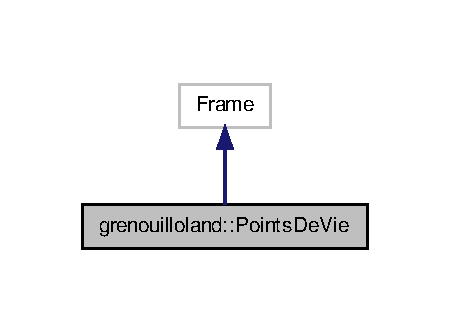
\includegraphics[width=216pt]{classgrenouilloland_1_1PointsDeVie__inherit__graph}
\end{center}
\end{figure}


Graphe de collaboration de grenouilloland\-:\-:Points\-De\-Vie\-:
\nopagebreak
\begin{figure}[H]
\begin{center}
\leavevmode
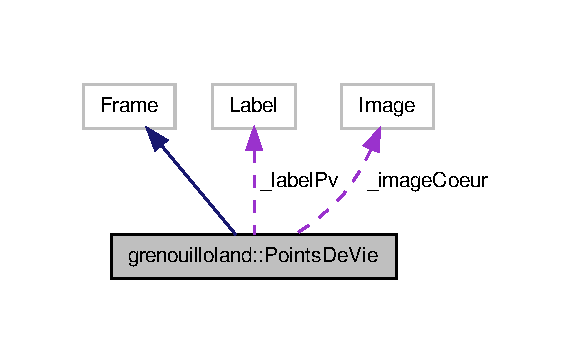
\includegraphics[width=274pt]{classgrenouilloland_1_1PointsDeVie__coll__graph}
\end{center}
\end{figure}
\subsection*{Fonctions membres publiques}
\begin{DoxyCompactItemize}
\item 
\hyperlink{classgrenouilloland_1_1PointsDeVie_a2e7343a93c85f829b632882f015cd683}{Points\-De\-Vie} (const Glib\-::ustring \&titre)
\end{DoxyCompactItemize}
\subsection*{Fonctions membres protégées}
\begin{DoxyCompactItemize}
\item 
void \hyperlink{classgrenouilloland_1_1PointsDeVie_a6fdc129a1d93e85ffae0f0ab948ce2ae}{mettre\-A\-Jour} (const \hyperlink{classgrenouilloland_1_1Presentateur}{Presentateur} \&presentateur)
\end{DoxyCompactItemize}
\subsection*{Attributs protégés}
\begin{DoxyCompactItemize}
\item 
Gtk\-::\-Image \hyperlink{classgrenouilloland_1_1PointsDeVie_a154df2e799b244ec1d0374af4297eb5d}{\-\_\-image\-Coeur}
\item 
Gtk\-::\-Label \hyperlink{classgrenouilloland_1_1PointsDeVie_a6b7f96b9a6eca2629c76ef30598c7b7b}{\-\_\-label\-Pv}
\end{DoxyCompactItemize}
\subsection*{Amis}
\begin{DoxyCompactItemize}
\item 
class \hyperlink{classgrenouilloland_1_1PointsDeVie_adc3b1810b8d3988a7832f57c330fe4fd}{Vue}
\end{DoxyCompactItemize}


\subsection{Description détaillée}
Afficheur des points de vie de la \hyperlink{classgrenouilloland_1_1Grenouille}{Grenouille}. 

\begin{DoxyAuthor}{Auteur}
Yann Dauxais 

Alexandre Beudin 
\end{DoxyAuthor}
\begin{DoxyDate}{Date}
6.\-1.\-2013
\end{DoxyDate}
Declaration de la classe \hyperlink{classgrenouilloland_1_1PointsDeVie}{Points\-De\-Vie} representant l'affichage des \hyperlink{classgrenouilloland_1_1PointsDeVie}{Points\-De\-Vie} et de la santé de la \hyperlink{classgrenouilloland_1_1Grenouille}{Grenouille}. Les Widget utilisés sont un label et une image.

\begin{DoxyNote}{Note}
une instance de cette classe ne peut etre dupliquee.

chaque instance de cette classe est son propre listener. 
\end{DoxyNote}


\subsection{Documentation des constructeurs et destructeur}
\hypertarget{classgrenouilloland_1_1PointsDeVie_a2e7343a93c85f829b632882f015cd683}{\index{grenouilloland\-::\-Points\-De\-Vie@{grenouilloland\-::\-Points\-De\-Vie}!Points\-De\-Vie@{Points\-De\-Vie}}
\index{Points\-De\-Vie@{Points\-De\-Vie}!grenouilloland::PointsDeVie@{grenouilloland\-::\-Points\-De\-Vie}}
\subsubsection[{Points\-De\-Vie}]{\setlength{\rightskip}{0pt plus 5cm}Points\-De\-Vie\-::\-Points\-De\-Vie (
\begin{DoxyParamCaption}
\item[{const Glib\-::ustring \&}]{titre}
\end{DoxyParamCaption}
)}}\label{classgrenouilloland_1_1PointsDeVie_a2e7343a93c85f829b632882f015cd683}
Constructeur logique.


\begin{DoxyParams}[1]{Paramètres}
\mbox{\tt in}  & {\em titre} & -\/ le titre du contour. \\
\hline
\end{DoxyParams}


\subsection{Documentation des fonctions membres}
\hypertarget{classgrenouilloland_1_1PointsDeVie_a6fdc129a1d93e85ffae0f0ab948ce2ae}{\index{grenouilloland\-::\-Points\-De\-Vie@{grenouilloland\-::\-Points\-De\-Vie}!mettre\-A\-Jour@{mettre\-A\-Jour}}
\index{mettre\-A\-Jour@{mettre\-A\-Jour}!grenouilloland::PointsDeVie@{grenouilloland\-::\-Points\-De\-Vie}}
\subsubsection[{mettre\-A\-Jour}]{\setlength{\rightskip}{0pt plus 5cm}void Points\-De\-Vie\-::mettre\-A\-Jour (
\begin{DoxyParamCaption}
\item[{const {\bf Presentateur} \&}]{presentateur}
\end{DoxyParamCaption}
)\hspace{0.3cm}{\ttfamily [protected]}}}\label{classgrenouilloland_1_1PointsDeVie_a6fdc129a1d93e85ffae0f0ab948ce2ae}
Met à jour l'image et le label selon l'état de la \hyperlink{classgrenouilloland_1_1Grenouille}{Grenouille} et son nombre de points de vie.


\begin{DoxyParams}[1]{Paramètres}
\mbox{\tt in}  & {\em presentateur} & -\/ le \hyperlink{classgrenouilloland_1_1Presentateur}{Presentateur} à invoquer. \\
\hline
\end{DoxyParams}


\subsection{Documentation des fonctions amies et associées}
\hypertarget{classgrenouilloland_1_1PointsDeVie_adc3b1810b8d3988a7832f57c330fe4fd}{\index{grenouilloland\-::\-Points\-De\-Vie@{grenouilloland\-::\-Points\-De\-Vie}!Vue@{Vue}}
\index{Vue@{Vue}!grenouilloland::PointsDeVie@{grenouilloland\-::\-Points\-De\-Vie}}
\subsubsection[{Vue}]{\setlength{\rightskip}{0pt plus 5cm}friend class {\bf Vue}\hspace{0.3cm}{\ttfamily [friend]}}}\label{classgrenouilloland_1_1PointsDeVie_adc3b1810b8d3988a7832f57c330fe4fd}
Declaration d'amitié. 

\subsection{Documentation des données membres}
\hypertarget{classgrenouilloland_1_1PointsDeVie_a154df2e799b244ec1d0374af4297eb5d}{\index{grenouilloland\-::\-Points\-De\-Vie@{grenouilloland\-::\-Points\-De\-Vie}!\-\_\-image\-Coeur@{\-\_\-image\-Coeur}}
\index{\-\_\-image\-Coeur@{\-\_\-image\-Coeur}!grenouilloland::PointsDeVie@{grenouilloland\-::\-Points\-De\-Vie}}
\subsubsection[{\-\_\-image\-Coeur}]{\setlength{\rightskip}{0pt plus 5cm}Gtk\-::\-Image grenouilloland\-::\-Points\-De\-Vie\-::\-\_\-image\-Coeur\hspace{0.3cm}{\ttfamily [protected]}}}\label{classgrenouilloland_1_1PointsDeVie_a154df2e799b244ec1d0374af4297eb5d}
Image. \hypertarget{classgrenouilloland_1_1PointsDeVie_a6b7f96b9a6eca2629c76ef30598c7b7b}{\index{grenouilloland\-::\-Points\-De\-Vie@{grenouilloland\-::\-Points\-De\-Vie}!\-\_\-label\-Pv@{\-\_\-label\-Pv}}
\index{\-\_\-label\-Pv@{\-\_\-label\-Pv}!grenouilloland::PointsDeVie@{grenouilloland\-::\-Points\-De\-Vie}}
\subsubsection[{\-\_\-label\-Pv}]{\setlength{\rightskip}{0pt plus 5cm}Gtk\-::\-Label grenouilloland\-::\-Points\-De\-Vie\-::\-\_\-label\-Pv\hspace{0.3cm}{\ttfamily [protected]}}}\label{classgrenouilloland_1_1PointsDeVie_a6b7f96b9a6eca2629c76ef30598c7b7b}
Label. 

La documentation de cette classe a été générée à partir des fichiers suivants \-:\begin{DoxyCompactItemize}
\item 
src/vue/include/Points\-De\-Vie.\-hh\item 
src/vue/Points\-De\-Vie.\-cpp\end{DoxyCompactItemize}

\hypertarget{classgrenouilloland_1_1Presentateur}{\section{Référence de la classe grenouilloland\-:\-:Presentateur}
\label{classgrenouilloland_1_1Presentateur}\index{grenouilloland\-::\-Presentateur@{grenouilloland\-::\-Presentateur}}
}


\hyperlink{classgrenouilloland_1_1Presentateur}{Presentateur} de l'application.  




{\ttfamily \#include $<$Presentateur.\-hh$>$}



Graphe de collaboration de grenouilloland\-:\-:Presentateur\-:
\nopagebreak
\begin{figure}[H]
\begin{center}
\leavevmode
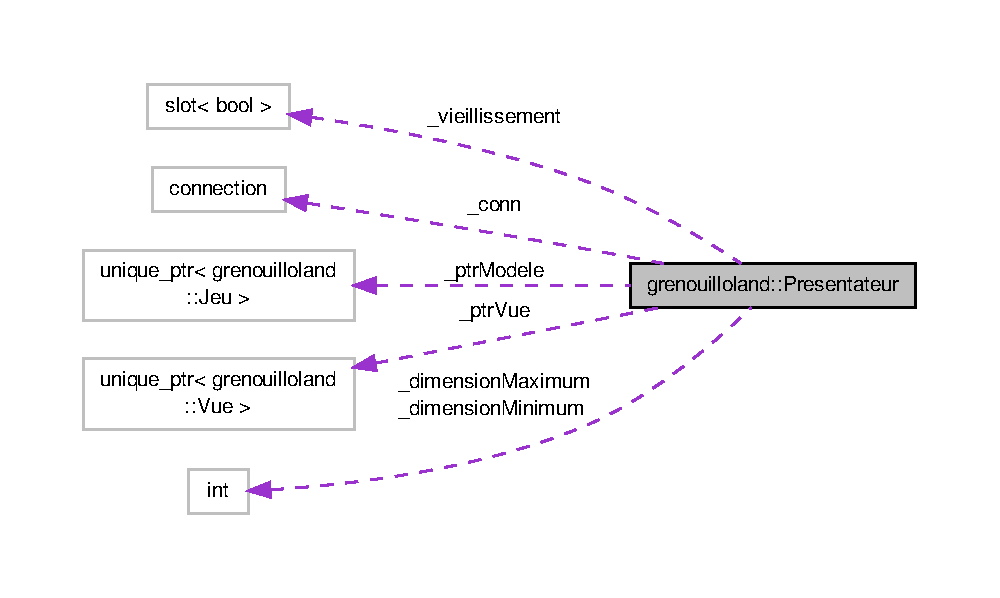
\includegraphics[width=350pt]{classgrenouilloland_1_1Presentateur__coll__graph}
\end{center}
\end{figure}
\subsection*{Classes}
\begin{DoxyCompactItemize}
\item 
class \hyperlink{classgrenouilloland_1_1Presentateur_1_1MandataireCaseGraphique}{Mandataire\-Case\-Graphique}
\begin{DoxyCompactList}\small\item\em \hyperlink{classgrenouilloland_1_1Presentateur_1_1MandataireCaseGraphique}{Mandataire\-Case\-Graphique} du \hyperlink{classgrenouilloland_1_1Presentateur}{Presentateur} du \hyperlink{classgrenouilloland_1_1Jeu}{Jeu} Grenouilloland. \end{DoxyCompactList}\item 
class \hyperlink{classgrenouilloland_1_1Presentateur_1_1MandataireVue}{Mandataire\-Vue}
\begin{DoxyCompactList}\small\item\em \hyperlink{classgrenouilloland_1_1Presentateur_1_1MandataireVue}{Mandataire\-Vue} du \hyperlink{classgrenouilloland_1_1Presentateur}{Presentateur} du \hyperlink{classgrenouilloland_1_1Jeu}{Jeu} Grenouilloland. \end{DoxyCompactList}\end{DoxyCompactItemize}
\subsection*{Fonctions membres publiques}
\begin{DoxyCompactItemize}
\item 
\hyperlink{classgrenouilloland_1_1Presentateur_aee3b0dd4271204ff0ea084a8851dfc5c}{Presentateur} (const int \&dimension\-Minimum, const int \&dimension\-Maximum, const int \&resolution)
\item 
const int \& \hyperlink{classgrenouilloland_1_1Presentateur_ad63992b986dc5e6c072f06c28ad4ef07}{lire\-Dimension\-Minimum} () const 
\item 
const int \& \hyperlink{classgrenouilloland_1_1Presentateur_ad9b094d2e8e65893d4bdaf02de8fc133}{lire\-Dimension\-Maximum} () const 
\item 
const \hyperlink{classgrenouilloland_1_1Jeu}{Jeu} \& \hyperlink{classgrenouilloland_1_1Presentateur_aecb0257a4af119e65be331478306cdac}{lire\-Modele} () const 
\item 
const \hyperlink{classgrenouilloland_1_1Vue}{Vue} \& \hyperlink{classgrenouilloland_1_1Presentateur_a47dc8cbc54d21a96d6a4aefb80b54b8d}{lire\-Vue} () const 
\item 
const int \& \hyperlink{classgrenouilloland_1_1Presentateur_a129a00656b36c61645dcc517eb6170b3}{dimension} () const 
\item 
void \hyperlink{classgrenouilloland_1_1Presentateur_a965ce165d6b8244e17d81226a5848e2d}{demarrer} ()
\end{DoxyCompactItemize}
\subsection*{Fonctions membres protégées}
\begin{DoxyCompactItemize}
\item 
void \hyperlink{classgrenouilloland_1_1Presentateur_afe66f32c7193c158209006bfd8f40627}{lancer\-Partie} ()
\item 
void \hyperlink{classgrenouilloland_1_1Presentateur_a37a714909d1e1813a497fa2da716332b}{nouveau\-Modele} (const int \&\hyperlink{classgrenouilloland_1_1Presentateur_a129a00656b36c61645dcc517eb6170b3}{dimension})
\item 
bool \hyperlink{classgrenouilloland_1_1Presentateur_aa4463c4fdb04f4852ce8e2ff32b0fe0b}{deplacer\-Grenouille} (const int \&ligne, const int \&colonne)
\item 
bool \hyperlink{classgrenouilloland_1_1Presentateur_ab3e69b7a51f4cb235bce31ec168f802c}{vieillissement} ()
\end{DoxyCompactItemize}
\subsection*{Attributs protégés}
\begin{DoxyCompactItemize}
\item 
const int \hyperlink{classgrenouilloland_1_1Presentateur_a94ac9459edd7299793d43196d42575f2}{\-\_\-dimension\-Minimum}
\item 
const int \hyperlink{classgrenouilloland_1_1Presentateur_a8d205215e5a4880713eb016dd1266a20}{\-\_\-dimension\-Maximum}
\item 
std\-::unique\-\_\-ptr$<$ \hyperlink{classgrenouilloland_1_1Jeu}{Jeu} $>$ \hyperlink{classgrenouilloland_1_1Presentateur_a3418c1b3461d7e4a511ac71bf30d2a14}{\-\_\-ptr\-Modele}
\item 
std\-::unique\-\_\-ptr$<$ \hyperlink{classgrenouilloland_1_1Vue}{Vue} $>$ \hyperlink{classgrenouilloland_1_1Presentateur_a806d2e46bff9428800f7b063015b792c}{\-\_\-ptr\-Vue}
\item 
sigc\-::connection \hyperlink{classgrenouilloland_1_1Presentateur_adecdbfff3ad277099345f4e768f95e50}{\-\_\-conn}
\item 
const sigc\-::slot$<$ bool $>$ \hyperlink{classgrenouilloland_1_1Presentateur_ad51c240a49a31b60bf36578a14860ae8}{\-\_\-vieillissement}
\end{DoxyCompactItemize}


\subsection{Description détaillée}
\hyperlink{classgrenouilloland_1_1Presentateur}{Presentateur} de l'application. 

\begin{DoxyAuthor}{Auteur}
Yann Dauxais 

Alexandre Beudin 
\end{DoxyAuthor}
\begin{DoxyDate}{Date}
6.\-1.\-2013
\end{DoxyDate}
Declaration de la classe \hyperlink{classgrenouilloland_1_1Presentateur}{Presentateur} representant le presentateur dans le modele d'archiecture graphique M\-V\-P.

\begin{DoxyNote}{Note}
une instance de cette classe ne peut etre dupliquee. 
\end{DoxyNote}


\subsection{Documentation des constructeurs et destructeur}
\hypertarget{classgrenouilloland_1_1Presentateur_aee3b0dd4271204ff0ea084a8851dfc5c}{\index{grenouilloland\-::\-Presentateur@{grenouilloland\-::\-Presentateur}!Presentateur@{Presentateur}}
\index{Presentateur@{Presentateur}!grenouilloland::Presentateur@{grenouilloland\-::\-Presentateur}}
\subsubsection[{Presentateur}]{\setlength{\rightskip}{0pt plus 5cm}Presentateur\-::\-Presentateur (
\begin{DoxyParamCaption}
\item[{const int \&}]{dimension\-Minimum, }
\item[{const int \&}]{dimension\-Maximum, }
\item[{const int \&}]{resolution}
\end{DoxyParamCaption}
)}}\label{classgrenouilloland_1_1Presentateur_aee3b0dd4271204ff0ea084a8851dfc5c}
Constructeur logique.


\begin{DoxyParams}[1]{Paramètres}
\mbox{\tt in}  & {\em dimension\-Minimum} & -\/ la valeur de \hyperlink{classgrenouilloland_1_1Presentateur_a94ac9459edd7299793d43196d42575f2}{\-\_\-dimension\-Minimum}. \\
\hline
\mbox{\tt in}  & {\em dimension\-Maximum} & -\/ la valeur de \hyperlink{classgrenouilloland_1_1Presentateur_a8d205215e5a4880713eb016dd1266a20}{\-\_\-dimension\-Maximum}. \\
\hline
\mbox{\tt in}  & {\em dimension} & -\/ la resolution initiale. \\
\hline
\end{DoxyParams}


\subsection{Documentation des fonctions membres}
\hypertarget{classgrenouilloland_1_1Presentateur_a965ce165d6b8244e17d81226a5848e2d}{\index{grenouilloland\-::\-Presentateur@{grenouilloland\-::\-Presentateur}!demarrer@{demarrer}}
\index{demarrer@{demarrer}!grenouilloland::Presentateur@{grenouilloland\-::\-Presentateur}}
\subsubsection[{demarrer}]{\setlength{\rightskip}{0pt plus 5cm}void Presentateur\-::demarrer (
\begin{DoxyParamCaption}
{}
\end{DoxyParamCaption}
)}}\label{classgrenouilloland_1_1Presentateur_a965ce165d6b8244e17d81226a5848e2d}
Demarre ce presentateur. \hypertarget{classgrenouilloland_1_1Presentateur_aa4463c4fdb04f4852ce8e2ff32b0fe0b}{\index{grenouilloland\-::\-Presentateur@{grenouilloland\-::\-Presentateur}!deplacer\-Grenouille@{deplacer\-Grenouille}}
\index{deplacer\-Grenouille@{deplacer\-Grenouille}!grenouilloland::Presentateur@{grenouilloland\-::\-Presentateur}}
\subsubsection[{deplacer\-Grenouille}]{\setlength{\rightskip}{0pt plus 5cm}bool Presentateur\-::deplacer\-Grenouille (
\begin{DoxyParamCaption}
\item[{const int \&}]{ligne, }
\item[{const int \&}]{colonne}
\end{DoxyParamCaption}
)\hspace{0.3cm}{\ttfamily [protected]}}}\label{classgrenouilloland_1_1Presentateur_aa4463c4fdb04f4852ce8e2ff32b0fe0b}
Déplace la grenouille dans le \hyperlink{classgrenouilloland_1_1Jeu}{Jeu}.


\begin{DoxyParams}[1]{Paramètres}
\mbox{\tt in}  & {\em ligne} & -\/ la ligne souhaitee. \\
\hline
\mbox{\tt in}  & {\em colonne} & -\/ la colonne souhaitee. \\
\hline
\end{DoxyParams}
\hypertarget{classgrenouilloland_1_1Presentateur_a129a00656b36c61645dcc517eb6170b3}{\index{grenouilloland\-::\-Presentateur@{grenouilloland\-::\-Presentateur}!dimension@{dimension}}
\index{dimension@{dimension}!grenouilloland::Presentateur@{grenouilloland\-::\-Presentateur}}
\subsubsection[{dimension}]{\setlength{\rightskip}{0pt plus 5cm}const int \& Presentateur\-::dimension (
\begin{DoxyParamCaption}
{}
\end{DoxyParamCaption}
) const}}\label{classgrenouilloland_1_1Presentateur_a129a00656b36c61645dcc517eb6170b3}
Retourne la dimension du modele associe a ce presentateur.

\begin{DoxyReturn}{Renvoie}
la dimension du modele associe a ce presentateur. 
\end{DoxyReturn}
\hypertarget{classgrenouilloland_1_1Presentateur_afe66f32c7193c158209006bfd8f40627}{\index{grenouilloland\-::\-Presentateur@{grenouilloland\-::\-Presentateur}!lancer\-Partie@{lancer\-Partie}}
\index{lancer\-Partie@{lancer\-Partie}!grenouilloland::Presentateur@{grenouilloland\-::\-Presentateur}}
\subsubsection[{lancer\-Partie}]{\setlength{\rightskip}{0pt plus 5cm}void Presentateur\-::lancer\-Partie (
\begin{DoxyParamCaption}
{}
\end{DoxyParamCaption}
)\hspace{0.3cm}{\ttfamily [protected]}}}\label{classgrenouilloland_1_1Presentateur_afe66f32c7193c158209006bfd8f40627}
Lance une nouvelle partie du \hyperlink{classgrenouilloland_1_1Jeu}{Jeu}. \hypertarget{classgrenouilloland_1_1Presentateur_ad9b094d2e8e65893d4bdaf02de8fc133}{\index{grenouilloland\-::\-Presentateur@{grenouilloland\-::\-Presentateur}!lire\-Dimension\-Maximum@{lire\-Dimension\-Maximum}}
\index{lire\-Dimension\-Maximum@{lire\-Dimension\-Maximum}!grenouilloland::Presentateur@{grenouilloland\-::\-Presentateur}}
\subsubsection[{lire\-Dimension\-Maximum}]{\setlength{\rightskip}{0pt plus 5cm}const int \& Presentateur\-::lire\-Dimension\-Maximum (
\begin{DoxyParamCaption}
{}
\end{DoxyParamCaption}
) const}}\label{classgrenouilloland_1_1Presentateur_ad9b094d2e8e65893d4bdaf02de8fc133}
Accesseur.

\begin{DoxyReturn}{Renvoie}
la valeur de \hyperlink{classgrenouilloland_1_1Presentateur_a8d205215e5a4880713eb016dd1266a20}{\-\_\-dimension\-Maximum}. 
\end{DoxyReturn}
\hypertarget{classgrenouilloland_1_1Presentateur_ad63992b986dc5e6c072f06c28ad4ef07}{\index{grenouilloland\-::\-Presentateur@{grenouilloland\-::\-Presentateur}!lire\-Dimension\-Minimum@{lire\-Dimension\-Minimum}}
\index{lire\-Dimension\-Minimum@{lire\-Dimension\-Minimum}!grenouilloland::Presentateur@{grenouilloland\-::\-Presentateur}}
\subsubsection[{lire\-Dimension\-Minimum}]{\setlength{\rightskip}{0pt plus 5cm}const int \& Presentateur\-::lire\-Dimension\-Minimum (
\begin{DoxyParamCaption}
{}
\end{DoxyParamCaption}
) const}}\label{classgrenouilloland_1_1Presentateur_ad63992b986dc5e6c072f06c28ad4ef07}
Accesseur.

\begin{DoxyReturn}{Renvoie}
la valeur de \hyperlink{classgrenouilloland_1_1Presentateur_a94ac9459edd7299793d43196d42575f2}{\-\_\-dimension\-Minimum}. 
\end{DoxyReturn}
\hypertarget{classgrenouilloland_1_1Presentateur_aecb0257a4af119e65be331478306cdac}{\index{grenouilloland\-::\-Presentateur@{grenouilloland\-::\-Presentateur}!lire\-Modele@{lire\-Modele}}
\index{lire\-Modele@{lire\-Modele}!grenouilloland::Presentateur@{grenouilloland\-::\-Presentateur}}
\subsubsection[{lire\-Modele}]{\setlength{\rightskip}{0pt plus 5cm}const {\bf Jeu} \& Presentateur\-::lire\-Modele (
\begin{DoxyParamCaption}
{}
\end{DoxyParamCaption}
) const}}\label{classgrenouilloland_1_1Presentateur_aecb0257a4af119e65be331478306cdac}
Accesseur.

\begin{DoxyReturn}{Renvoie}
la valeur de \hyperlink{classgrenouilloland_1_1Presentateur_a3418c1b3461d7e4a511ac71bf30d2a14}{\-\_\-ptr\-Modele}. 
\end{DoxyReturn}
\hypertarget{classgrenouilloland_1_1Presentateur_a47dc8cbc54d21a96d6a4aefb80b54b8d}{\index{grenouilloland\-::\-Presentateur@{grenouilloland\-::\-Presentateur}!lire\-Vue@{lire\-Vue}}
\index{lire\-Vue@{lire\-Vue}!grenouilloland::Presentateur@{grenouilloland\-::\-Presentateur}}
\subsubsection[{lire\-Vue}]{\setlength{\rightskip}{0pt plus 5cm}const {\bf Vue} \& Presentateur\-::lire\-Vue (
\begin{DoxyParamCaption}
{}
\end{DoxyParamCaption}
) const}}\label{classgrenouilloland_1_1Presentateur_a47dc8cbc54d21a96d6a4aefb80b54b8d}
Accesseur.

\begin{DoxyReturn}{Renvoie}
la valeur de \hyperlink{classgrenouilloland_1_1Presentateur_a806d2e46bff9428800f7b063015b792c}{\-\_\-ptr\-Vue}. 
\end{DoxyReturn}
\hypertarget{classgrenouilloland_1_1Presentateur_a37a714909d1e1813a497fa2da716332b}{\index{grenouilloland\-::\-Presentateur@{grenouilloland\-::\-Presentateur}!nouveau\-Modele@{nouveau\-Modele}}
\index{nouveau\-Modele@{nouveau\-Modele}!grenouilloland::Presentateur@{grenouilloland\-::\-Presentateur}}
\subsubsection[{nouveau\-Modele}]{\setlength{\rightskip}{0pt plus 5cm}void Presentateur\-::nouveau\-Modele (
\begin{DoxyParamCaption}
\item[{const int \&}]{dimension}
\end{DoxyParamCaption}
)\hspace{0.3cm}{\ttfamily [protected]}}}\label{classgrenouilloland_1_1Presentateur_a37a714909d1e1813a497fa2da716332b}
Change le modele associe a ce presentateur.


\begin{DoxyParams}[1]{Paramètres}
\mbox{\tt in}  & {\em dimension} & -\/ la dimension souhaitee. \\
\hline
\end{DoxyParams}
\hypertarget{classgrenouilloland_1_1Presentateur_ab3e69b7a51f4cb235bce31ec168f802c}{\index{grenouilloland\-::\-Presentateur@{grenouilloland\-::\-Presentateur}!vieillissement@{vieillissement}}
\index{vieillissement@{vieillissement}!grenouilloland::Presentateur@{grenouilloland\-::\-Presentateur}}
\subsubsection[{vieillissement}]{\setlength{\rightskip}{0pt plus 5cm}bool Presentateur\-::vieillissement (
\begin{DoxyParamCaption}
{}
\end{DoxyParamCaption}
)\hspace{0.3cm}{\ttfamily [protected]}}}\label{classgrenouilloland_1_1Presentateur_ab3e69b7a51f4cb235bce31ec168f802c}
Lance le vieillissement des éléments du \hyperlink{classgrenouilloland_1_1Jeu}{Jeu}. 

\subsection{Documentation des données membres}
\hypertarget{classgrenouilloland_1_1Presentateur_adecdbfff3ad277099345f4e768f95e50}{\index{grenouilloland\-::\-Presentateur@{grenouilloland\-::\-Presentateur}!\-\_\-conn@{\-\_\-conn}}
\index{\-\_\-conn@{\-\_\-conn}!grenouilloland::Presentateur@{grenouilloland\-::\-Presentateur}}
\subsubsection[{\-\_\-conn}]{\setlength{\rightskip}{0pt plus 5cm}sigc\-::connection grenouilloland\-::\-Presentateur\-::\-\_\-conn\hspace{0.3cm}{\ttfamily [protected]}}}\label{classgrenouilloland_1_1Presentateur_adecdbfff3ad277099345f4e768f95e50}
Connecteur de slot à un évènement. \hypertarget{classgrenouilloland_1_1Presentateur_a8d205215e5a4880713eb016dd1266a20}{\index{grenouilloland\-::\-Presentateur@{grenouilloland\-::\-Presentateur}!\-\_\-dimension\-Maximum@{\-\_\-dimension\-Maximum}}
\index{\-\_\-dimension\-Maximum@{\-\_\-dimension\-Maximum}!grenouilloland::Presentateur@{grenouilloland\-::\-Presentateur}}
\subsubsection[{\-\_\-dimension\-Maximum}]{\setlength{\rightskip}{0pt plus 5cm}const int grenouilloland\-::\-Presentateur\-::\-\_\-dimension\-Maximum\hspace{0.3cm}{\ttfamily [protected]}}}\label{classgrenouilloland_1_1Presentateur_a8d205215e5a4880713eb016dd1266a20}
\hyperlink{classgrenouilloland_1_1Dimension}{Dimension} maximum du modele. \hypertarget{classgrenouilloland_1_1Presentateur_a94ac9459edd7299793d43196d42575f2}{\index{grenouilloland\-::\-Presentateur@{grenouilloland\-::\-Presentateur}!\-\_\-dimension\-Minimum@{\-\_\-dimension\-Minimum}}
\index{\-\_\-dimension\-Minimum@{\-\_\-dimension\-Minimum}!grenouilloland::Presentateur@{grenouilloland\-::\-Presentateur}}
\subsubsection[{\-\_\-dimension\-Minimum}]{\setlength{\rightskip}{0pt plus 5cm}const int grenouilloland\-::\-Presentateur\-::\-\_\-dimension\-Minimum\hspace{0.3cm}{\ttfamily [protected]}}}\label{classgrenouilloland_1_1Presentateur_a94ac9459edd7299793d43196d42575f2}
\hyperlink{classgrenouilloland_1_1Dimension}{Dimension} minimum du modele. \hypertarget{classgrenouilloland_1_1Presentateur_a3418c1b3461d7e4a511ac71bf30d2a14}{\index{grenouilloland\-::\-Presentateur@{grenouilloland\-::\-Presentateur}!\-\_\-ptr\-Modele@{\-\_\-ptr\-Modele}}
\index{\-\_\-ptr\-Modele@{\-\_\-ptr\-Modele}!grenouilloland::Presentateur@{grenouilloland\-::\-Presentateur}}
\subsubsection[{\-\_\-ptr\-Modele}]{\setlength{\rightskip}{0pt plus 5cm}std\-::unique\-\_\-ptr$<$ {\bf Jeu} $>$ grenouilloland\-::\-Presentateur\-::\-\_\-ptr\-Modele\hspace{0.3cm}{\ttfamily [protected]}}}\label{classgrenouilloland_1_1Presentateur_a3418c1b3461d7e4a511ac71bf30d2a14}
Modele associe a ce presentateur. \hypertarget{classgrenouilloland_1_1Presentateur_a806d2e46bff9428800f7b063015b792c}{\index{grenouilloland\-::\-Presentateur@{grenouilloland\-::\-Presentateur}!\-\_\-ptr\-Vue@{\-\_\-ptr\-Vue}}
\index{\-\_\-ptr\-Vue@{\-\_\-ptr\-Vue}!grenouilloland::Presentateur@{grenouilloland\-::\-Presentateur}}
\subsubsection[{\-\_\-ptr\-Vue}]{\setlength{\rightskip}{0pt plus 5cm}std\-::unique\-\_\-ptr$<$ {\bf Vue} $>$ grenouilloland\-::\-Presentateur\-::\-\_\-ptr\-Vue\hspace{0.3cm}{\ttfamily [protected]}}}\label{classgrenouilloland_1_1Presentateur_a806d2e46bff9428800f7b063015b792c}
\hyperlink{classgrenouilloland_1_1Vue}{Vue} associee a ce presentateur. \hypertarget{classgrenouilloland_1_1Presentateur_ad51c240a49a31b60bf36578a14860ae8}{\index{grenouilloland\-::\-Presentateur@{grenouilloland\-::\-Presentateur}!\-\_\-vieillissement@{\-\_\-vieillissement}}
\index{\-\_\-vieillissement@{\-\_\-vieillissement}!grenouilloland::Presentateur@{grenouilloland\-::\-Presentateur}}
\subsubsection[{\-\_\-vieillissement}]{\setlength{\rightskip}{0pt plus 5cm}const sigc\-::slot$<$bool$>$ grenouilloland\-::\-Presentateur\-::\-\_\-vieillissement\hspace{0.3cm}{\ttfamily [protected]}}}\label{classgrenouilloland_1_1Presentateur_ad51c240a49a31b60bf36578a14860ae8}
Slot qui sera attaché à la méthode vieillissement. 

La documentation de cette classe a été générée à partir des fichiers suivants \-:\begin{DoxyCompactItemize}
\item 
src/presentateur/include/Presentateur.\-hh\item 
src/presentateur/Presentateur.\-cpp\end{DoxyCompactItemize}

\hypertarget{classgrenouilloland_1_1StrategieAbstraite}{\section{Référence de la classe grenouilloland\-:\-:Strategie\-Abstraite}
\label{classgrenouilloland_1_1StrategieAbstraite}\index{grenouilloland\-::\-Strategie\-Abstraite@{grenouilloland\-::\-Strategie\-Abstraite}}
}


\hyperlink{classgrenouilloland_1_1StrategieAbstraite}{Strategie\-Abstraite} du \hyperlink{classgrenouilloland_1_1Jeu}{Jeu} Grenouilloland.  




{\ttfamily \#include $<$Strategie\-Abstraite.\-hh$>$}



Graphe d'héritage de grenouilloland\-:\-:Strategie\-Abstraite\-:
\nopagebreak
\begin{figure}[H]
\begin{center}
\leavevmode
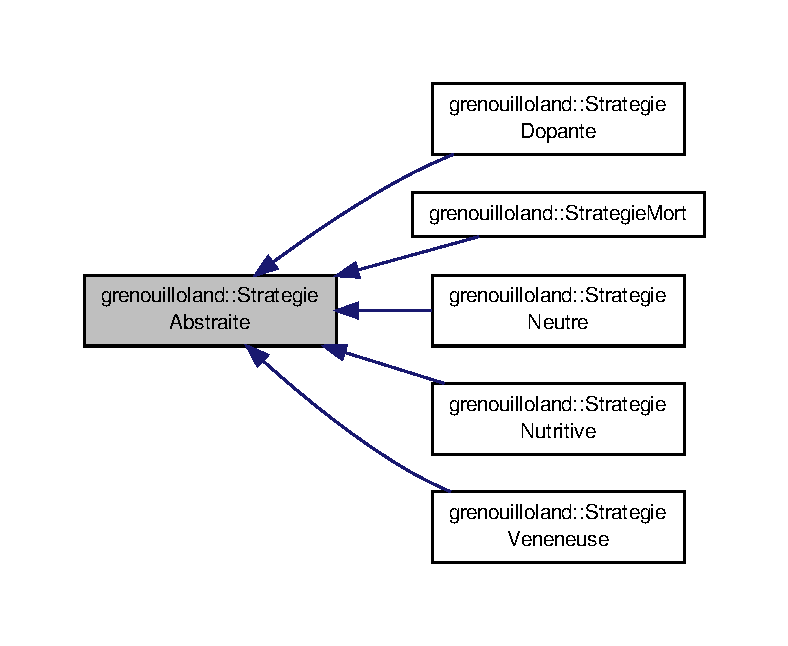
\includegraphics[width=350pt]{classgrenouilloland_1_1StrategieAbstraite__inherit__graph}
\end{center}
\end{figure}
\subsection*{Fonctions membres publiques}
\begin{DoxyCompactItemize}
\item 
void \hyperlink{classgrenouilloland_1_1StrategieAbstraite_a00d3b038cba36687274e6fec37d28417}{appliquer\-Strategie} (\hyperlink{classgrenouilloland_1_1Grenouille}{Grenouille} \&g) const 
\item 
virtual void \hyperlink{classgrenouilloland_1_1StrategieAbstraite_a1355917a007ab0c5e5ed358e2eee93c2}{appliquer\-Effet} (unsigned int \&pv, bool \&malade) const =0
\end{DoxyCompactItemize}


\subsection{Description détaillée}
\hyperlink{classgrenouilloland_1_1StrategieAbstraite}{Strategie\-Abstraite} du \hyperlink{classgrenouilloland_1_1Jeu}{Jeu} Grenouilloland. 

\begin{DoxyAuthor}{Auteur}
Beudin.\-Alexandre Dauxais.\-Yann 
\end{DoxyAuthor}
\begin{DoxyDate}{Date}
05.\-01.\-2012
\end{DoxyDate}
Declaration de la classe abstraite \hyperlink{classgrenouilloland_1_1StrategieAbstraite}{Strategie\-Abstraite} réprésentant la structure d'une stratégie du jeu Grenouilloland. 

\subsection{Documentation des fonctions membres}
\hypertarget{classgrenouilloland_1_1StrategieAbstraite_a1355917a007ab0c5e5ed358e2eee93c2}{\index{grenouilloland\-::\-Strategie\-Abstraite@{grenouilloland\-::\-Strategie\-Abstraite}!appliquer\-Effet@{appliquer\-Effet}}
\index{appliquer\-Effet@{appliquer\-Effet}!grenouilloland::StrategieAbstraite@{grenouilloland\-::\-Strategie\-Abstraite}}
\subsubsection[{appliquer\-Effet}]{\setlength{\rightskip}{0pt plus 5cm}virtual void grenouilloland\-::\-Strategie\-Abstraite\-::appliquer\-Effet (
\begin{DoxyParamCaption}
\item[{unsigned int \&}]{pv, }
\item[{bool \&}]{malade}
\end{DoxyParamCaption}
) const\hspace{0.3cm}{\ttfamily [pure virtual]}}}\label{classgrenouilloland_1_1StrategieAbstraite_a1355917a007ab0c5e5ed358e2eee93c2}
Application des effets de la stratégie.


\begin{DoxyParams}[1]{Paramètres}
\mbox{\tt in,out}  & {\em pv} & -\/ pv à modifier. \\
\hline
\mbox{\tt in,out}  & {\em malade} & -\/ état de santé à modifier. \\
\hline
\end{DoxyParams}


Implémenté dans \hyperlink{classgrenouilloland_1_1StrategieDopante_a68860bdaf9afa8e4ded568bf56314051}{grenouilloland\-::\-Strategie\-Dopante}, \hyperlink{classgrenouilloland_1_1StrategieMort_aef9dc1d5ce3195c955d9da69af806957}{grenouilloland\-::\-Strategie\-Mort}, \hyperlink{classgrenouilloland_1_1StrategieNeutre_a8e6c41ebe5ed9c0477ad3e203f766567}{grenouilloland\-::\-Strategie\-Neutre}, \hyperlink{classgrenouilloland_1_1StrategieNutritive_aa7338486cae06a62f5f155d72f40ab87}{grenouilloland\-::\-Strategie\-Nutritive}, et \hyperlink{classgrenouilloland_1_1StrategieVeneneuse_a13de8092ed7e5561cf5833693deaf662}{grenouilloland\-::\-Strategie\-Veneneuse}.

\hypertarget{classgrenouilloland_1_1StrategieAbstraite_a00d3b038cba36687274e6fec37d28417}{\index{grenouilloland\-::\-Strategie\-Abstraite@{grenouilloland\-::\-Strategie\-Abstraite}!appliquer\-Strategie@{appliquer\-Strategie}}
\index{appliquer\-Strategie@{appliquer\-Strategie}!grenouilloland::StrategieAbstraite@{grenouilloland\-::\-Strategie\-Abstraite}}
\subsubsection[{appliquer\-Strategie}]{\setlength{\rightskip}{0pt plus 5cm}void Strategie\-Abstraite\-::appliquer\-Strategie (
\begin{DoxyParamCaption}
\item[{{\bf Grenouille} \&}]{g}
\end{DoxyParamCaption}
) const}}\label{classgrenouilloland_1_1StrategieAbstraite_a00d3b038cba36687274e6fec37d28417}
Application de la stratégie sur une grenouille.


\begin{DoxyParams}[1]{Paramètres}
\mbox{\tt in,out}  & {\em g} & -\/ grenouille subissant la stratégie. \\
\hline
\end{DoxyParams}


La documentation de cette classe a été générée à partir des fichiers suivants \-:\begin{DoxyCompactItemize}
\item 
src/modele/include/Strategie\-Abstraite.\-hh\item 
src/modele/Strategie\-Abstraite.\-cpp\end{DoxyCompactItemize}

\hypertarget{classgrenouilloland_1_1StrategieDopante}{\section{Référence de la classe grenouilloland\-:\-:Strategie\-Dopante}
\label{classgrenouilloland_1_1StrategieDopante}\index{grenouilloland\-::\-Strategie\-Dopante@{grenouilloland\-::\-Strategie\-Dopante}}
}


\hyperlink{classgrenouilloland_1_1StrategieDopante}{Strategie\-Dopante} du \hyperlink{classgrenouilloland_1_1Jeu}{Jeu} Grenouilloland.  




{\ttfamily \#include $<$Strategie\-Dopante.\-hh$>$}



Graphe d'héritage de grenouilloland\-:\-:Strategie\-Dopante\-:
\nopagebreak
\begin{figure}[H]
\begin{center}
\leavevmode
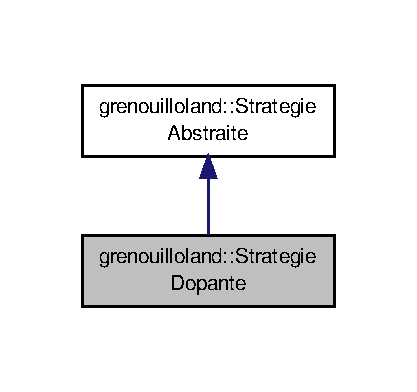
\includegraphics[width=200pt]{classgrenouilloland_1_1StrategieDopante__inherit__graph}
\end{center}
\end{figure}


Graphe de collaboration de grenouilloland\-:\-:Strategie\-Dopante\-:
\nopagebreak
\begin{figure}[H]
\begin{center}
\leavevmode
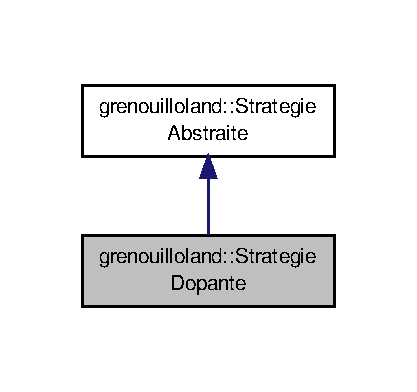
\includegraphics[width=200pt]{classgrenouilloland_1_1StrategieDopante__coll__graph}
\end{center}
\end{figure}
\subsection*{Classes}
\begin{DoxyCompactItemize}
\item 
class \hyperlink{classgrenouilloland_1_1StrategieDopante_1_1Mandataire}{Mandataire}
\begin{DoxyCompactList}\small\item\em \hyperlink{classgrenouilloland_1_1StrategieDopante_1_1Mandataire}{Mandataire} de \hyperlink{classgrenouilloland_1_1StrategieDopante}{Strategie\-Dopante} du \hyperlink{classgrenouilloland_1_1Jeu}{Jeu} Grenouilloland. \end{DoxyCompactList}\end{DoxyCompactItemize}
\subsection*{Fonctions membres publiques}
\begin{DoxyCompactItemize}
\item 
void \hyperlink{classgrenouilloland_1_1StrategieDopante_a68860bdaf9afa8e4ded568bf56314051}{appliquer\-Effet} (unsigned int \&pv, bool \&malade) const 
\end{DoxyCompactItemize}


\subsection{Description détaillée}
\hyperlink{classgrenouilloland_1_1StrategieDopante}{Strategie\-Dopante} du \hyperlink{classgrenouilloland_1_1Jeu}{Jeu} Grenouilloland. 

\begin{DoxyAuthor}{Auteur}
Beudin.\-Alexandre Dauxais.\-Yann 
\end{DoxyAuthor}
\begin{DoxyDate}{Date}
05.\-01.\-2012
\end{DoxyDate}
Declaration de la classe \hyperlink{classgrenouilloland_1_1StrategieDopante}{Strategie\-Dopante} réprésentant la stratégie dopante d'un nénuphar du jeu Grenouilloland. 

\subsection{Documentation des fonctions membres}
\hypertarget{classgrenouilloland_1_1StrategieDopante_a68860bdaf9afa8e4ded568bf56314051}{\index{grenouilloland\-::\-Strategie\-Dopante@{grenouilloland\-::\-Strategie\-Dopante}!appliquer\-Effet@{appliquer\-Effet}}
\index{appliquer\-Effet@{appliquer\-Effet}!grenouilloland::StrategieDopante@{grenouilloland\-::\-Strategie\-Dopante}}
\subsubsection[{appliquer\-Effet}]{\setlength{\rightskip}{0pt plus 5cm}void Strategie\-Dopante\-::appliquer\-Effet (
\begin{DoxyParamCaption}
\item[{unsigned int \&}]{pv, }
\item[{bool \&}]{malade}
\end{DoxyParamCaption}
) const\hspace{0.3cm}{\ttfamily [virtual]}}}\label{classgrenouilloland_1_1StrategieDopante_a68860bdaf9afa8e4ded568bf56314051}
Application des effets de la stratégie.


\begin{DoxyParams}[1]{Paramètres}
\mbox{\tt in,out}  & {\em pv} & -\/ pv à modifier. \\
\hline
\mbox{\tt in,out}  & {\em malade} & -\/ état de santé à modifier. \\
\hline
\end{DoxyParams}


Implémente \hyperlink{classgrenouilloland_1_1StrategieAbstraite_a1355917a007ab0c5e5ed358e2eee93c2}{grenouilloland\-::\-Strategie\-Abstraite}.



La documentation de cette classe a été générée à partir des fichiers suivants \-:\begin{DoxyCompactItemize}
\item 
src/modele/include/Strategie\-Dopante.\-hh\item 
src/modele/Strategie\-Dopante.\-cpp\end{DoxyCompactItemize}

\hypertarget{classgrenouilloland_1_1StrategieMort}{\section{Référence de la classe grenouilloland\-:\-:Strategie\-Mort}
\label{classgrenouilloland_1_1StrategieMort}\index{grenouilloland\-::\-Strategie\-Mort@{grenouilloland\-::\-Strategie\-Mort}}
}


\hyperlink{classgrenouilloland_1_1StrategieMort}{Strategie\-Mort} du \hyperlink{classgrenouilloland_1_1Jeu}{Jeu} Grenouilloland.  




{\ttfamily \#include $<$Strategie\-Mort.\-hh$>$}



Graphe d'héritage de grenouilloland\-:\-:Strategie\-Mort\-:
\nopagebreak
\begin{figure}[H]
\begin{center}
\leavevmode
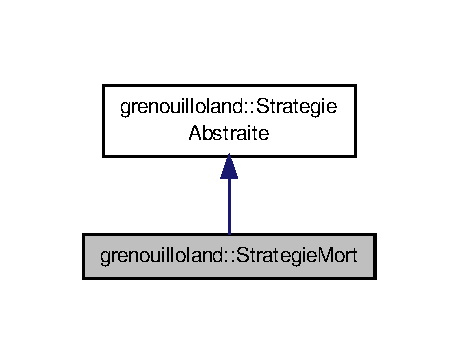
\includegraphics[width=220pt]{classgrenouilloland_1_1StrategieMort__inherit__graph}
\end{center}
\end{figure}


Graphe de collaboration de grenouilloland\-:\-:Strategie\-Mort\-:
\nopagebreak
\begin{figure}[H]
\begin{center}
\leavevmode
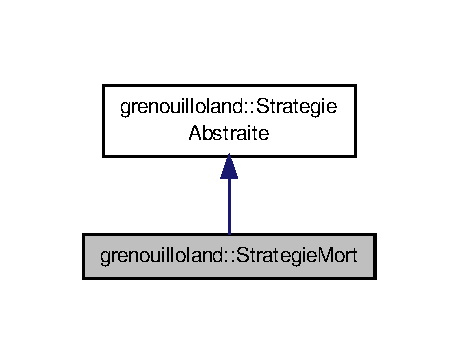
\includegraphics[width=220pt]{classgrenouilloland_1_1StrategieMort__coll__graph}
\end{center}
\end{figure}
\subsection*{Classes}
\begin{DoxyCompactItemize}
\item 
class \hyperlink{classgrenouilloland_1_1StrategieMort_1_1Mandataire}{Mandataire}
\begin{DoxyCompactList}\small\item\em \hyperlink{classgrenouilloland_1_1StrategieMort_1_1Mandataire}{Mandataire} de \hyperlink{classgrenouilloland_1_1StrategieMort}{Strategie\-Mort} du \hyperlink{classgrenouilloland_1_1Jeu}{Jeu} Grenouilloland. \end{DoxyCompactList}\end{DoxyCompactItemize}
\subsection*{Fonctions membres publiques}
\begin{DoxyCompactItemize}
\item 
void \hyperlink{classgrenouilloland_1_1StrategieMort_aef9dc1d5ce3195c955d9da69af806957}{appliquer\-Effet} (unsigned int \&pv, bool \&malade) const 
\end{DoxyCompactItemize}


\subsection{Description détaillée}
\hyperlink{classgrenouilloland_1_1StrategieMort}{Strategie\-Mort} du \hyperlink{classgrenouilloland_1_1Jeu}{Jeu} Grenouilloland. 

\begin{DoxyAuthor}{Auteur}
Beudin.\-Alexandre Dauxais.\-Yann 
\end{DoxyAuthor}
\begin{DoxyDate}{Date}
05.\-01.\-2012
\end{DoxyDate}
Declaration de la classe \hyperlink{classgrenouilloland_1_1StrategieMort}{Strategie\-Mort} réprésentant la stratégie de mort d'un nénuphar du jeu Grenouilloland. 

\subsection{Documentation des fonctions membres}
\hypertarget{classgrenouilloland_1_1StrategieMort_aef9dc1d5ce3195c955d9da69af806957}{\index{grenouilloland\-::\-Strategie\-Mort@{grenouilloland\-::\-Strategie\-Mort}!appliquer\-Effet@{appliquer\-Effet}}
\index{appliquer\-Effet@{appliquer\-Effet}!grenouilloland::StrategieMort@{grenouilloland\-::\-Strategie\-Mort}}
\subsubsection[{appliquer\-Effet}]{\setlength{\rightskip}{0pt plus 5cm}void Strategie\-Mort\-::appliquer\-Effet (
\begin{DoxyParamCaption}
\item[{unsigned int \&}]{pv, }
\item[{bool \&}]{malade}
\end{DoxyParamCaption}
) const\hspace{0.3cm}{\ttfamily [virtual]}}}\label{classgrenouilloland_1_1StrategieMort_aef9dc1d5ce3195c955d9da69af806957}
Application des effets de la stratégie.


\begin{DoxyParams}[1]{Paramètres}
\mbox{\tt in,out}  & {\em pv} & -\/ pv à modifier. \\
\hline
\mbox{\tt in,out}  & {\em malade} & -\/ état de santé à modifier. \\
\hline
\end{DoxyParams}


Implémente \hyperlink{classgrenouilloland_1_1StrategieAbstraite_a1355917a007ab0c5e5ed358e2eee93c2}{grenouilloland\-::\-Strategie\-Abstraite}.



La documentation de cette classe a été générée à partir des fichiers suivants \-:\begin{DoxyCompactItemize}
\item 
src/modele/include/Strategie\-Mort.\-hh\item 
src/modele/Strategie\-Mort.\-cpp\end{DoxyCompactItemize}

\hypertarget{classgrenouilloland_1_1StrategieNeutre}{\section{Référence de la classe grenouilloland\-:\-:Strategie\-Neutre}
\label{classgrenouilloland_1_1StrategieNeutre}\index{grenouilloland\-::\-Strategie\-Neutre@{grenouilloland\-::\-Strategie\-Neutre}}
}


\hyperlink{classgrenouilloland_1_1StrategieNeutre}{Strategie\-Neutre} du \hyperlink{classgrenouilloland_1_1Jeu}{Jeu} Grenouilloland.  




{\ttfamily \#include $<$Strategie\-Neutre.\-hh$>$}



Graphe d'héritage de grenouilloland\-:\-:Strategie\-Neutre\-:
\nopagebreak
\begin{figure}[H]
\begin{center}
\leavevmode
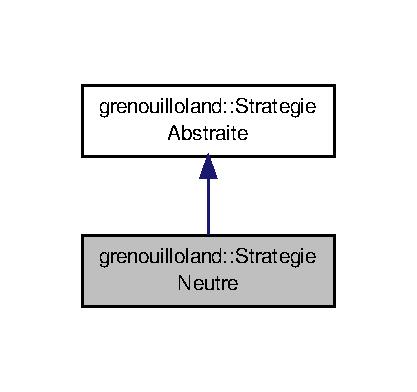
\includegraphics[width=200pt]{classgrenouilloland_1_1StrategieNeutre__inherit__graph}
\end{center}
\end{figure}


Graphe de collaboration de grenouilloland\-:\-:Strategie\-Neutre\-:
\nopagebreak
\begin{figure}[H]
\begin{center}
\leavevmode
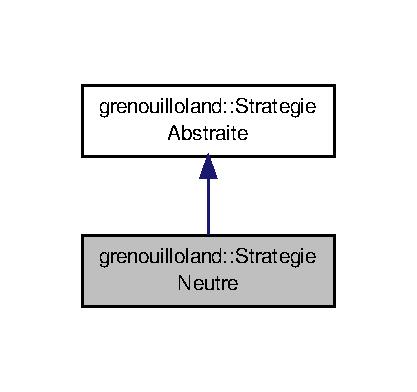
\includegraphics[width=200pt]{classgrenouilloland_1_1StrategieNeutre__coll__graph}
\end{center}
\end{figure}
\subsection*{Classes}
\begin{DoxyCompactItemize}
\item 
class \hyperlink{classgrenouilloland_1_1StrategieNeutre_1_1Mandataire}{Mandataire}
\begin{DoxyCompactList}\small\item\em \hyperlink{classgrenouilloland_1_1StrategieNeutre_1_1Mandataire}{Mandataire} de \hyperlink{classgrenouilloland_1_1StrategieNeutre}{Strategie\-Neutre} du \hyperlink{classgrenouilloland_1_1Jeu}{Jeu} Grenouilloland. \end{DoxyCompactList}\end{DoxyCompactItemize}
\subsection*{Fonctions membres publiques}
\begin{DoxyCompactItemize}
\item 
void \hyperlink{classgrenouilloland_1_1StrategieNeutre_a8e6c41ebe5ed9c0477ad3e203f766567}{appliquer\-Effet} (unsigned int \&pv, bool \&malade) const 
\end{DoxyCompactItemize}


\subsection{Description détaillée}
\hyperlink{classgrenouilloland_1_1StrategieNeutre}{Strategie\-Neutre} du \hyperlink{classgrenouilloland_1_1Jeu}{Jeu} Grenouilloland. 

\begin{DoxyAuthor}{Auteur}
Beudin.\-Alexandre Dauxais.\-Yann 
\end{DoxyAuthor}
\begin{DoxyDate}{Date}
05.\-01.\-2012
\end{DoxyDate}
Declaration de la classe \hyperlink{classgrenouilloland_1_1StrategieNeutre}{Strategie\-Neutre} réprésentant la stratégie neutre d'un nénuphar du jeu Grenouilloland. 

\subsection{Documentation des fonctions membres}
\hypertarget{classgrenouilloland_1_1StrategieNeutre_a8e6c41ebe5ed9c0477ad3e203f766567}{\index{grenouilloland\-::\-Strategie\-Neutre@{grenouilloland\-::\-Strategie\-Neutre}!appliquer\-Effet@{appliquer\-Effet}}
\index{appliquer\-Effet@{appliquer\-Effet}!grenouilloland::StrategieNeutre@{grenouilloland\-::\-Strategie\-Neutre}}
\subsubsection[{appliquer\-Effet}]{\setlength{\rightskip}{0pt plus 5cm}void Strategie\-Neutre\-::appliquer\-Effet (
\begin{DoxyParamCaption}
\item[{unsigned int \&}]{pv, }
\item[{bool \&}]{malade}
\end{DoxyParamCaption}
) const\hspace{0.3cm}{\ttfamily [virtual]}}}\label{classgrenouilloland_1_1StrategieNeutre_a8e6c41ebe5ed9c0477ad3e203f766567}
Application des effets de la stratégie.


\begin{DoxyParams}[1]{Paramètres}
\mbox{\tt in,out}  & {\em pv} & -\/ pv à modifier. \\
\hline
\mbox{\tt in,out}  & {\em malade} & -\/ état de santé à modifier. \\
\hline
\end{DoxyParams}


Implémente \hyperlink{classgrenouilloland_1_1StrategieAbstraite_a1355917a007ab0c5e5ed358e2eee93c2}{grenouilloland\-::\-Strategie\-Abstraite}.



La documentation de cette classe a été générée à partir des fichiers suivants \-:\begin{DoxyCompactItemize}
\item 
src/modele/include/Strategie\-Neutre.\-hh\item 
src/modele/Strategie\-Neutre.\-cpp\end{DoxyCompactItemize}

\hypertarget{classgrenouilloland_1_1StrategieNutritive}{\section{Référence de la classe grenouilloland\-:\-:Strategie\-Nutritive}
\label{classgrenouilloland_1_1StrategieNutritive}\index{grenouilloland\-::\-Strategie\-Nutritive@{grenouilloland\-::\-Strategie\-Nutritive}}
}


\hyperlink{classgrenouilloland_1_1StrategieNutritive}{Strategie\-Nutritive} du \hyperlink{classgrenouilloland_1_1Jeu}{Jeu} Grenouilloland.  




{\ttfamily \#include $<$Strategie\-Nutritive.\-hh$>$}



Graphe d'héritage de grenouilloland\-:\-:Strategie\-Nutritive\-:
\nopagebreak
\begin{figure}[H]
\begin{center}
\leavevmode
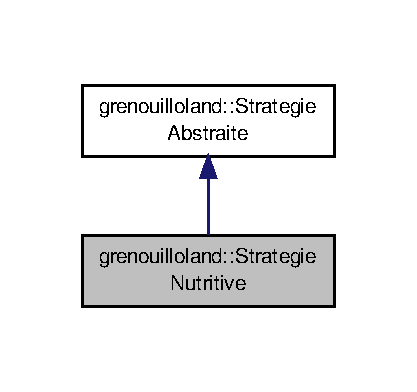
\includegraphics[width=200pt]{classgrenouilloland_1_1StrategieNutritive__inherit__graph}
\end{center}
\end{figure}


Graphe de collaboration de grenouilloland\-:\-:Strategie\-Nutritive\-:
\nopagebreak
\begin{figure}[H]
\begin{center}
\leavevmode
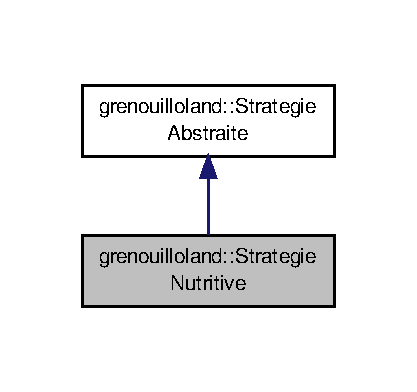
\includegraphics[width=200pt]{classgrenouilloland_1_1StrategieNutritive__coll__graph}
\end{center}
\end{figure}
\subsection*{Classes}
\begin{DoxyCompactItemize}
\item 
class \hyperlink{classgrenouilloland_1_1StrategieNutritive_1_1Mandataire}{Mandataire}
\begin{DoxyCompactList}\small\item\em \hyperlink{classgrenouilloland_1_1StrategieNutritive_1_1Mandataire}{Mandataire} de \hyperlink{classgrenouilloland_1_1StrategieNutritive}{Strategie\-Nutritive} du \hyperlink{classgrenouilloland_1_1Jeu}{Jeu} Grenouilloland. \end{DoxyCompactList}\end{DoxyCompactItemize}
\subsection*{Fonctions membres publiques}
\begin{DoxyCompactItemize}
\item 
void \hyperlink{classgrenouilloland_1_1StrategieNutritive_aa7338486cae06a62f5f155d72f40ab87}{appliquer\-Effet} (unsigned int \&pv, bool \&malade) const 
\end{DoxyCompactItemize}


\subsection{Description détaillée}
\hyperlink{classgrenouilloland_1_1StrategieNutritive}{Strategie\-Nutritive} du \hyperlink{classgrenouilloland_1_1Jeu}{Jeu} Grenouilloland. 

\begin{DoxyAuthor}{Auteur}
Beudin.\-Alexandre Dauxais.\-Yann 
\end{DoxyAuthor}
\begin{DoxyDate}{Date}
05.\-01.\-2012
\end{DoxyDate}
Declaration de la classe \hyperlink{classgrenouilloland_1_1StrategieNutritive}{Strategie\-Nutritive} réprésentant la stratégie nutritive d'un nénuphar du jeu Grenouilloland. 

\subsection{Documentation des fonctions membres}
\hypertarget{classgrenouilloland_1_1StrategieNutritive_aa7338486cae06a62f5f155d72f40ab87}{\index{grenouilloland\-::\-Strategie\-Nutritive@{grenouilloland\-::\-Strategie\-Nutritive}!appliquer\-Effet@{appliquer\-Effet}}
\index{appliquer\-Effet@{appliquer\-Effet}!grenouilloland::StrategieNutritive@{grenouilloland\-::\-Strategie\-Nutritive}}
\subsubsection[{appliquer\-Effet}]{\setlength{\rightskip}{0pt plus 5cm}void Strategie\-Nutritive\-::appliquer\-Effet (
\begin{DoxyParamCaption}
\item[{unsigned int \&}]{pv, }
\item[{bool \&}]{malade}
\end{DoxyParamCaption}
) const\hspace{0.3cm}{\ttfamily [virtual]}}}\label{classgrenouilloland_1_1StrategieNutritive_aa7338486cae06a62f5f155d72f40ab87}
Application des effets de la stratégie.


\begin{DoxyParams}[1]{Paramètres}
\mbox{\tt in,out}  & {\em pv} & -\/ pv à modifier. \\
\hline
\mbox{\tt in,out}  & {\em malade} & -\/ état de santé à modifier. \\
\hline
\end{DoxyParams}


Implémente \hyperlink{classgrenouilloland_1_1StrategieAbstraite_a1355917a007ab0c5e5ed358e2eee93c2}{grenouilloland\-::\-Strategie\-Abstraite}.



La documentation de cette classe a été générée à partir des fichiers suivants \-:\begin{DoxyCompactItemize}
\item 
src/modele/include/Strategie\-Nutritive.\-hh\item 
src/modele/Strategie\-Nutritive.\-cpp\end{DoxyCompactItemize}

\hypertarget{classgrenouilloland_1_1StrategieVeneneuse}{\section{Référence de la classe grenouilloland\-:\-:Strategie\-Veneneuse}
\label{classgrenouilloland_1_1StrategieVeneneuse}\index{grenouilloland\-::\-Strategie\-Veneneuse@{grenouilloland\-::\-Strategie\-Veneneuse}}
}


\hyperlink{classgrenouilloland_1_1StrategieVeneneuse}{Strategie\-Veneneuse} du \hyperlink{classgrenouilloland_1_1Jeu}{Jeu} Grenouilloland.  




{\ttfamily \#include $<$Strategie\-Veneneuse.\-hh$>$}



Graphe d'héritage de grenouilloland\-:\-:Strategie\-Veneneuse\-:
\nopagebreak
\begin{figure}[H]
\begin{center}
\leavevmode
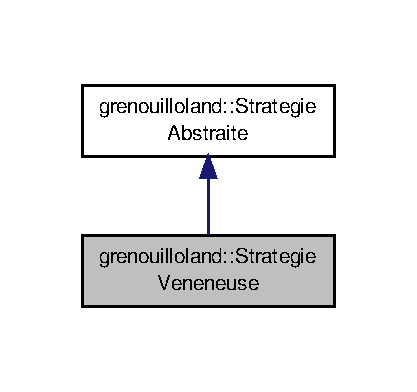
\includegraphics[width=200pt]{classgrenouilloland_1_1StrategieVeneneuse__inherit__graph}
\end{center}
\end{figure}


Graphe de collaboration de grenouilloland\-:\-:Strategie\-Veneneuse\-:
\nopagebreak
\begin{figure}[H]
\begin{center}
\leavevmode
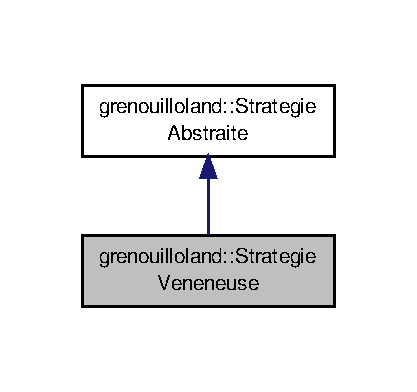
\includegraphics[width=200pt]{classgrenouilloland_1_1StrategieVeneneuse__coll__graph}
\end{center}
\end{figure}
\subsection*{Classes}
\begin{DoxyCompactItemize}
\item 
class \hyperlink{classgrenouilloland_1_1StrategieVeneneuse_1_1Mandataire}{Mandataire}
\begin{DoxyCompactList}\small\item\em \hyperlink{classgrenouilloland_1_1StrategieVeneneuse_1_1Mandataire}{Mandataire} de \hyperlink{classgrenouilloland_1_1StrategieVeneneuse}{Strategie\-Veneneuse} du \hyperlink{classgrenouilloland_1_1Jeu}{Jeu} Grenouilloland. \end{DoxyCompactList}\end{DoxyCompactItemize}
\subsection*{Fonctions membres publiques}
\begin{DoxyCompactItemize}
\item 
void \hyperlink{classgrenouilloland_1_1StrategieVeneneuse_a13de8092ed7e5561cf5833693deaf662}{appliquer\-Effet} (unsigned int \&pv, bool \&malade) const 
\end{DoxyCompactItemize}


\subsection{Description détaillée}
\hyperlink{classgrenouilloland_1_1StrategieVeneneuse}{Strategie\-Veneneuse} du \hyperlink{classgrenouilloland_1_1Jeu}{Jeu} Grenouilloland. 

\begin{DoxyAuthor}{Auteur}
Beudin.\-Alexandre Dauxais.\-Yann 
\end{DoxyAuthor}
\begin{DoxyDate}{Date}
05.\-01.\-2012
\end{DoxyDate}
Declaration de la classe \hyperlink{classgrenouilloland_1_1StrategieVeneneuse}{Strategie\-Veneneuse} réprésentant la stratégie vénéneuse d'un nénuphar du jeu Grenouilloland. 

\subsection{Documentation des fonctions membres}
\hypertarget{classgrenouilloland_1_1StrategieVeneneuse_a13de8092ed7e5561cf5833693deaf662}{\index{grenouilloland\-::\-Strategie\-Veneneuse@{grenouilloland\-::\-Strategie\-Veneneuse}!appliquer\-Effet@{appliquer\-Effet}}
\index{appliquer\-Effet@{appliquer\-Effet}!grenouilloland::StrategieVeneneuse@{grenouilloland\-::\-Strategie\-Veneneuse}}
\subsubsection[{appliquer\-Effet}]{\setlength{\rightskip}{0pt plus 5cm}void Strategie\-Veneneuse\-::appliquer\-Effet (
\begin{DoxyParamCaption}
\item[{unsigned int \&}]{pv, }
\item[{bool \&}]{malade}
\end{DoxyParamCaption}
) const\hspace{0.3cm}{\ttfamily [virtual]}}}\label{classgrenouilloland_1_1StrategieVeneneuse_a13de8092ed7e5561cf5833693deaf662}
Application des effets de la stratégie.


\begin{DoxyParams}[1]{Paramètres}
\mbox{\tt in,out}  & {\em pv} & -\/ pv à modifier. \\
\hline
\mbox{\tt in,out}  & {\em malade} & -\/ état de santé à modifier. \\
\hline
\end{DoxyParams}


Implémente \hyperlink{classgrenouilloland_1_1StrategieAbstraite_a1355917a007ab0c5e5ed358e2eee93c2}{grenouilloland\-::\-Strategie\-Abstraite}.



La documentation de cette classe a été générée à partir des fichiers suivants \-:\begin{DoxyCompactItemize}
\item 
src/modele/include/Strategie\-Veneneuse.\-hh\item 
src/modele/Strategie\-Veneneuse.\-cpp\end{DoxyCompactItemize}

\hypertarget{classgrenouilloland_1_1Vue}{\section{Référence de la classe grenouilloland\-:\-:Vue}
\label{classgrenouilloland_1_1Vue}\index{grenouilloland\-::\-Vue@{grenouilloland\-::\-Vue}}
}


\hyperlink{classgrenouilloland_1_1Vue}{Vue} de l'application.  




{\ttfamily \#include $<$Vue.\-hh$>$}



Graphe d'héritage de grenouilloland\-:\-:Vue\-:
\nopagebreak
\begin{figure}[H]
\begin{center}
\leavevmode
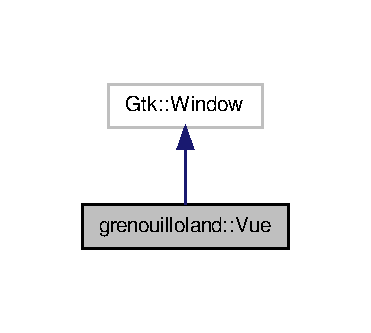
\includegraphics[width=178pt]{classgrenouilloland_1_1Vue__inherit__graph}
\end{center}
\end{figure}


Graphe de collaboration de grenouilloland\-:\-:Vue\-:
\nopagebreak
\begin{figure}[H]
\begin{center}
\leavevmode
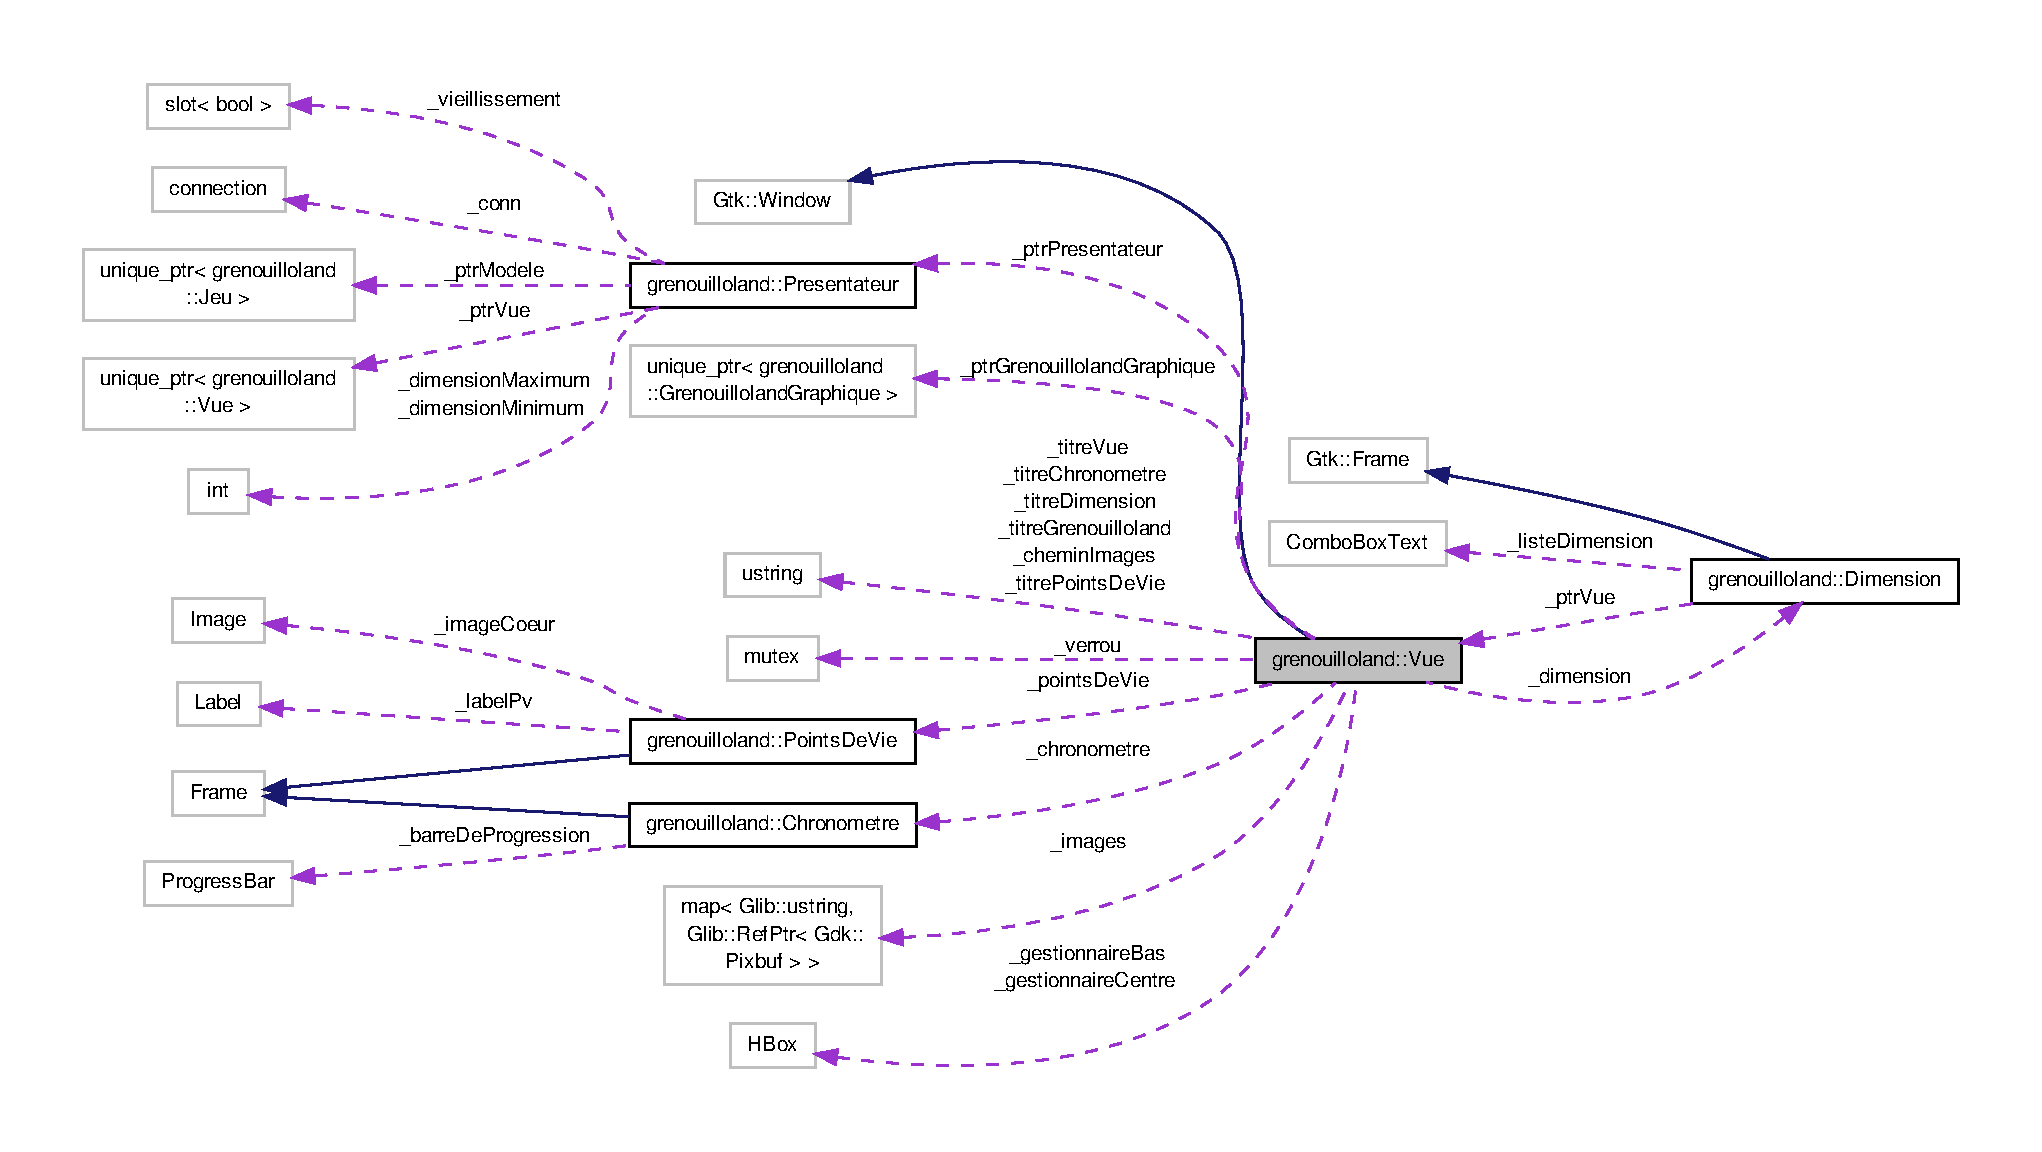
\includegraphics[width=350pt]{classgrenouilloland_1_1Vue__coll__graph}
\end{center}
\end{figure}
\subsection*{Classes}
\begin{DoxyCompactItemize}
\item 
class \hyperlink{classgrenouilloland_1_1Vue_1_1Mandataire}{Mandataire}
\end{DoxyCompactItemize}
\subsection*{Fonctions membres publiques}
\begin{DoxyCompactItemize}
\item 
\hyperlink{classgrenouilloland_1_1Vue_a757da0d74ff38e0c6f95408ca48290df}{Vue} (\hyperlink{classgrenouilloland_1_1Presentateur}{Presentateur} \&presentateur)
\item 
const \hyperlink{classgrenouilloland_1_1Presentateur}{Presentateur} \& \hyperlink{classgrenouilloland_1_1Vue_a9ef1dcf95036a43bec9284168924a653}{lire\-Presentateur} () const 
\end{DoxyCompactItemize}
\subsection*{Fonctions membres publiques statiques}
\begin{DoxyCompactItemize}
\item 
static void \hyperlink{classgrenouilloland_1_1Vue_afdd453417b5b374129e27d739750d449}{initialiser} ()
\item 
static const Glib\-::ustring \hyperlink{classgrenouilloland_1_1Vue_a223dad39b984bc48648a69cb97b5ff6e}{lire\-Titre\-Vue} ()
\item 
static const Glib\-::ustring \hyperlink{classgrenouilloland_1_1Vue_a1c46be867356f059d3b96b909920963b}{lire\-Titre\-Grenouilloland} ()
\item 
static const Glib\-::ustring \hyperlink{classgrenouilloland_1_1Vue_a36b09d267fb47c48ca326ea88c0e946c}{lire\-Titre\-Points\-De\-Vie} ()
\item 
static const Glib\-::ustring \hyperlink{classgrenouilloland_1_1Vue_a88c78d10cc710d33358a3176e26faa51}{lire\-Titre\-Chronometre} ()
\item 
static const Glib\-::ustring \hyperlink{classgrenouilloland_1_1Vue_adf5485ae9e2d418cffe7c27d273affa8}{lire\-Titre\-Dimension} ()
\end{DoxyCompactItemize}
\subsection*{Fonctions membres protégées}
\begin{DoxyCompactItemize}
\item 
void \hyperlink{classgrenouilloland_1_1Vue_a05dde5184e07bb61266e311b5fca58e6}{mettre\-A\-Jour} ()
\item 
\hyperlink{classgrenouilloland_1_1Presentateur}{Presentateur} \& \hyperlink{classgrenouilloland_1_1Vue_a69daf9edcf49ae15bb1d593f642bde07}{lire\-Presentateur\-Modifiable} ()
\item 
void \hyperlink{classgrenouilloland_1_1Vue_a8d220428da4420cdb0bf039c915412ac}{verrouiller} ()
\item 
void \hyperlink{classgrenouilloland_1_1Vue_a6fa4cd2dc80413b819679fdd24ba7e2e}{deverrouiller} ()
\item 
void \hyperlink{classgrenouilloland_1_1Vue_a6f7d83c684de2e51c2536d74614c6a21}{construire\-Barre\-Menus\-Et\-Outils} (Gtk\-::\-V\-Box \&gestionnaire)
\item 
void \hyperlink{classgrenouilloland_1_1Vue_a5020ff24aa99091a71f8b812be8578dc}{construire\-Partie\-Centrale} (Gtk\-::\-V\-Box \&gestionnaire)
\item 
void \hyperlink{classgrenouilloland_1_1Vue_ac2f033ddbd1508798f748e8fb816eb34}{construire\-Partie\-Inferieure} (Gtk\-::\-V\-Box \&gestionnaire)
\item 
void \hyperlink{classgrenouilloland_1_1Vue_a094c688903d968d9366460a5431a0130}{cb\-Nouveau} ()
\item 
void \hyperlink{classgrenouilloland_1_1Vue_a253d6db7fc7664d060025cd03d9566d4}{cb\-Changer\-Modele} ()
\item 
void \hyperlink{classgrenouilloland_1_1Vue_a3b30a58e0986b5ad9368a85995a39293}{cb\-A\-Propos} ()
\item 
void \hyperlink{classgrenouilloland_1_1Vue_a136783ac8ab9e7085630e9db4924a189}{cb\-Quitter} ()
\end{DoxyCompactItemize}
\subsection*{Fonctions membres protégées statiques}
\begin{DoxyCompactItemize}
\item 
static const Glib\-::\-Ref\-Ptr\\*
$<$ Gdk\-::\-Pixbuf $>$ \& \hyperlink{classgrenouilloland_1_1Vue_a13bd0ca693c418c7b5ee30ac7be56448}{lire\-Image} (const Glib\-::ustring \&nom)
\end{DoxyCompactItemize}
\subsection*{Attributs protégés}
\begin{DoxyCompactItemize}
\item 
\hyperlink{classgrenouilloland_1_1Presentateur}{Presentateur} $\ast$const \hyperlink{classgrenouilloland_1_1Vue_a18b21aec8d74287eb28374399827c022}{\-\_\-ptr\-Presentateur}
\item 
std\-::unique\-\_\-ptr\\*
$<$ \hyperlink{classgrenouilloland_1_1GrenouillolandGraphique}{Grenouilloland\-Graphique} $>$ \hyperlink{classgrenouilloland_1_1Vue_a998feee5bed8136f999d2e3484d0c6ca}{\-\_\-ptr\-Grenouilloland\-Graphique}
\item 
\hyperlink{classgrenouilloland_1_1PointsDeVie}{Points\-De\-Vie} \hyperlink{classgrenouilloland_1_1Vue_af6f2bba3b33001e5c0807d8e98c0b0fa}{\-\_\-points\-De\-Vie}
\item 
\hyperlink{classgrenouilloland_1_1Dimension}{Dimension} \hyperlink{classgrenouilloland_1_1Vue_a8913ac00882895d6a0552edc92266883}{\-\_\-dimension}
\item 
\hyperlink{classgrenouilloland_1_1Chronometre}{Chronometre} \hyperlink{classgrenouilloland_1_1Vue_a6632cb40512ad2d01c9a52b33de24aeb}{\-\_\-chronometre}
\item 
Gtk\-::\-H\-Box \hyperlink{classgrenouilloland_1_1Vue_a64a3b9c74425f9a70fbae4c5bc7d9c78}{\-\_\-gestionnaire\-Centre}
\item 
Gtk\-::\-H\-Box \hyperlink{classgrenouilloland_1_1Vue_a65d5b3129325746ee1d1dbf0c3f3e0db}{\-\_\-gestionnaire\-Bas}
\item 
std\-::mutex \hyperlink{classgrenouilloland_1_1Vue_ab6f850d86942bdef050596e90a34494e}{\-\_\-verrou}
\end{DoxyCompactItemize}
\subsection*{Attributs protégés statiques}
\begin{DoxyCompactItemize}
\item 
static const Glib\-::ustring \hyperlink{classgrenouilloland_1_1Vue_a5adfea17feebe0674431b82d8215240e}{\-\_\-titre\-Vue}
\item 
static const Glib\-::ustring \hyperlink{classgrenouilloland_1_1Vue_a8f48d405d345306684f25471c377be4b}{\-\_\-titre\-Grenouilloland}
\item 
static const Glib\-::ustring \hyperlink{classgrenouilloland_1_1Vue_adc86530a0f01ba959d5dcd48a96f8b95}{\-\_\-titre\-Points\-De\-Vie}
\item 
static const Glib\-::ustring \hyperlink{classgrenouilloland_1_1Vue_af6206813ed4886372538752ddbaa746c}{\-\_\-titre\-Chronometre}
\item 
static const Glib\-::ustring \hyperlink{classgrenouilloland_1_1Vue_a233d73dd3c303194933f0da4d3749efe}{\-\_\-titre\-Dimension}
\item 
static const Glib\-::ustring \hyperlink{classgrenouilloland_1_1Vue_a2129d9ff7713d6b8d8c2cd444c6c7344}{\-\_\-chemin\-Images}
\item 
static std\-::map$<$ Glib\-::ustring, \\*
Glib\-::\-Ref\-Ptr$<$ Gdk\-::\-Pixbuf $>$ $>$ \hyperlink{classgrenouilloland_1_1Vue_a1ad2483d0795c038267934208730d415}{\-\_\-images}
\end{DoxyCompactItemize}
\subsection*{Amis}
\begin{DoxyCompactItemize}
\item 
class \hyperlink{classgrenouilloland_1_1Vue_ac12b0ba9ebe667c8408ac35bf21598e8}{Case\-Graphique}
\item 
class \hyperlink{classgrenouilloland_1_1Vue_aabae1fdc220bf040d4f5c2c057abfcf5}{Dimension}
\item 
class \hyperlink{classgrenouilloland_1_1Vue_a2f6a9fb1ac6fc3eaae981e0630df21d8}{Points\-De\-Vie}
\end{DoxyCompactItemize}


\subsection{Description détaillée}
\hyperlink{classgrenouilloland_1_1Vue}{Vue} de l'application. 

\begin{DoxyAuthor}{Auteur}
Yann Dauxais 

Alexandre Beudin 
\end{DoxyAuthor}
\begin{DoxyDate}{Date}
6.\-1.\-2013
\end{DoxyDate}
Declaration de la classe \hyperlink{classgrenouilloland_1_1Vue}{Vue} representant la vue de l'application, c'est a dire son interface graphique.

\begin{DoxyNote}{Note}
Une instance de cette classe ne peut etre dupliquee. 
\end{DoxyNote}


\subsection{Documentation des constructeurs et destructeur}
\hypertarget{classgrenouilloland_1_1Vue_a757da0d74ff38e0c6f95408ca48290df}{\index{grenouilloland\-::\-Vue@{grenouilloland\-::\-Vue}!Vue@{Vue}}
\index{Vue@{Vue}!grenouilloland::Vue@{grenouilloland\-::\-Vue}}
\subsubsection[{Vue}]{\setlength{\rightskip}{0pt plus 5cm}Vue\-::\-Vue (
\begin{DoxyParamCaption}
\item[{{\bf Presentateur} \&}]{presentateur}
\end{DoxyParamCaption}
)}}\label{classgrenouilloland_1_1Vue_a757da0d74ff38e0c6f95408ca48290df}
Constructeur logique.


\begin{DoxyParams}[1]{Paramètres}
\mbox{\tt in}  & {\em presentateur} & -\/ la valeur de \hyperlink{classgrenouilloland_1_1Vue_a18b21aec8d74287eb28374399827c022}{\-\_\-ptr\-Presentateur}. \\
\hline
\end{DoxyParams}


\subsection{Documentation des fonctions membres}
\hypertarget{classgrenouilloland_1_1Vue_a3b30a58e0986b5ad9368a85995a39293}{\index{grenouilloland\-::\-Vue@{grenouilloland\-::\-Vue}!cb\-A\-Propos@{cb\-A\-Propos}}
\index{cb\-A\-Propos@{cb\-A\-Propos}!grenouilloland::Vue@{grenouilloland\-::\-Vue}}
\subsubsection[{cb\-A\-Propos}]{\setlength{\rightskip}{0pt plus 5cm}void Vue\-::cb\-A\-Propos (
\begin{DoxyParamCaption}
{}
\end{DoxyParamCaption}
)\hspace{0.3cm}{\ttfamily [protected]}}}\label{classgrenouilloland_1_1Vue_a3b30a58e0986b5ad9368a85995a39293}
Callback permettant de presenter l'application et ses auteurs. Cette methode est invoquee suite a un click sur l'entree \char`\"{}\-A propos ...\char`\"{} du menu \char`\"{}\-Commandes\char`\"{} ou bien sur le bouton correspondant dans la barre d'outils. \hypertarget{classgrenouilloland_1_1Vue_a253d6db7fc7664d060025cd03d9566d4}{\index{grenouilloland\-::\-Vue@{grenouilloland\-::\-Vue}!cb\-Changer\-Modele@{cb\-Changer\-Modele}}
\index{cb\-Changer\-Modele@{cb\-Changer\-Modele}!grenouilloland::Vue@{grenouilloland\-::\-Vue}}
\subsubsection[{cb\-Changer\-Modele}]{\setlength{\rightskip}{0pt plus 5cm}void Vue\-::cb\-Changer\-Modele (
\begin{DoxyParamCaption}
{}
\end{DoxyParamCaption}
)\hspace{0.3cm}{\ttfamily [protected]}}}\label{classgrenouilloland_1_1Vue_a253d6db7fc7664d060025cd03d9566d4}
Callback permettant de preparer une nouvelle partie avec une autre dimension. Cette methode est invoquee par le controleur de la resolution du jeu.

\begin{DoxyNote}{Note}
Cette methode verrouille cette vue pendant toute son execution. 
\end{DoxyNote}
\hypertarget{classgrenouilloland_1_1Vue_a094c688903d968d9366460a5431a0130}{\index{grenouilloland\-::\-Vue@{grenouilloland\-::\-Vue}!cb\-Nouveau@{cb\-Nouveau}}
\index{cb\-Nouveau@{cb\-Nouveau}!grenouilloland::Vue@{grenouilloland\-::\-Vue}}
\subsubsection[{cb\-Nouveau}]{\setlength{\rightskip}{0pt plus 5cm}void Vue\-::cb\-Nouveau (
\begin{DoxyParamCaption}
{}
\end{DoxyParamCaption}
)\hspace{0.3cm}{\ttfamily [protected]}}}\label{classgrenouilloland_1_1Vue_a094c688903d968d9366460a5431a0130}
Callback permettant de preparer le jeu pour une nouvelle partie. Cette methode est invoquee suite a un click sur l'entree \char`\"{}\-Nouveau\char`\"{} du menu \char`\"{}\-Commandes\char`\"{} ou bien sur le bouton correspondant dans la barre d'outils.

\begin{DoxyNote}{Note}
Cette methode verrouille cette vue pendant toute son execution. 
\end{DoxyNote}
\hypertarget{classgrenouilloland_1_1Vue_a136783ac8ab9e7085630e9db4924a189}{\index{grenouilloland\-::\-Vue@{grenouilloland\-::\-Vue}!cb\-Quitter@{cb\-Quitter}}
\index{cb\-Quitter@{cb\-Quitter}!grenouilloland::Vue@{grenouilloland\-::\-Vue}}
\subsubsection[{cb\-Quitter}]{\setlength{\rightskip}{0pt plus 5cm}void Vue\-::cb\-Quitter (
\begin{DoxyParamCaption}
{}
\end{DoxyParamCaption}
)\hspace{0.3cm}{\ttfamily [protected]}}}\label{classgrenouilloland_1_1Vue_a136783ac8ab9e7085630e9db4924a189}
Callback permettant de quitter proprement l'application. Cette methode est invoquee suite a un click sur l'entree \char`\"{}\-Quitter\char`\"{} du menu \char`\"{}\-Commandes\char`\"{} ou bien sur le bouton correspondant dans la barre d'outils.

\begin{DoxyNote}{Note}
Cette methode verrouille cette vue pendant toute son execution. 
\end{DoxyNote}
\hypertarget{classgrenouilloland_1_1Vue_a6f7d83c684de2e51c2536d74614c6a21}{\index{grenouilloland\-::\-Vue@{grenouilloland\-::\-Vue}!construire\-Barre\-Menus\-Et\-Outils@{construire\-Barre\-Menus\-Et\-Outils}}
\index{construire\-Barre\-Menus\-Et\-Outils@{construire\-Barre\-Menus\-Et\-Outils}!grenouilloland::Vue@{grenouilloland\-::\-Vue}}
\subsubsection[{construire\-Barre\-Menus\-Et\-Outils}]{\setlength{\rightskip}{0pt plus 5cm}void Vue\-::construire\-Barre\-Menus\-Et\-Outils (
\begin{DoxyParamCaption}
\item[{Gtk\-::\-V\-Box \&}]{gestionnaire}
\end{DoxyParamCaption}
)\hspace{0.3cm}{\ttfamily [protected]}}}\label{classgrenouilloland_1_1Vue_a6f7d83c684de2e51c2536d74614c6a21}
Construit les barre de menus et d'outils.


\begin{DoxyParams}[1]{Paramètres}
\mbox{\tt in,out}  & {\em gestionnaire} & -\/ le gestionnaire de mise en forme associe a la fenetre principale. \\
\hline
\end{DoxyParams}
\hypertarget{classgrenouilloland_1_1Vue_a5020ff24aa99091a71f8b812be8578dc}{\index{grenouilloland\-::\-Vue@{grenouilloland\-::\-Vue}!construire\-Partie\-Centrale@{construire\-Partie\-Centrale}}
\index{construire\-Partie\-Centrale@{construire\-Partie\-Centrale}!grenouilloland::Vue@{grenouilloland\-::\-Vue}}
\subsubsection[{construire\-Partie\-Centrale}]{\setlength{\rightskip}{0pt plus 5cm}void Vue\-::construire\-Partie\-Centrale (
\begin{DoxyParamCaption}
\item[{Gtk\-::\-V\-Box \&}]{gestionnaire}
\end{DoxyParamCaption}
)\hspace{0.3cm}{\ttfamily [protected]}}}\label{classgrenouilloland_1_1Vue_a5020ff24aa99091a71f8b812be8578dc}
Construit la partie centrale de la fenetre principale contenant le \hyperlink{classgrenouilloland_1_1GrenouillolandGraphique}{Grenouilloland\-Graphique} et le panneau d'affichage des \hyperlink{classgrenouilloland_1_1PointsDeVie}{Points\-De\-Vie}.


\begin{DoxyParams}[1]{Paramètres}
\mbox{\tt in,out}  & {\em gestionnaire} & -\/ le gestionnaire de mise en forme associe a la fenetre principale. \\
\hline
\end{DoxyParams}
\hypertarget{classgrenouilloland_1_1Vue_ac2f033ddbd1508798f748e8fb816eb34}{\index{grenouilloland\-::\-Vue@{grenouilloland\-::\-Vue}!construire\-Partie\-Inferieure@{construire\-Partie\-Inferieure}}
\index{construire\-Partie\-Inferieure@{construire\-Partie\-Inferieure}!grenouilloland::Vue@{grenouilloland\-::\-Vue}}
\subsubsection[{construire\-Partie\-Inferieure}]{\setlength{\rightskip}{0pt plus 5cm}void Vue\-::construire\-Partie\-Inferieure (
\begin{DoxyParamCaption}
\item[{Gtk\-::\-V\-Box \&}]{gestionnaire}
\end{DoxyParamCaption}
)\hspace{0.3cm}{\ttfamily [protected]}}}\label{classgrenouilloland_1_1Vue_ac2f033ddbd1508798f748e8fb816eb34}
Construit la partie inferieure de la fenetre principale contenant le controleur de la dimension du jeu.


\begin{DoxyParams}[1]{Paramètres}
\mbox{\tt in,out}  & {\em gestionnaire} & -\/ le gestionnaire de mise en forme associe a la fenetre principale. \\
\hline
\end{DoxyParams}
\hypertarget{classgrenouilloland_1_1Vue_a6fa4cd2dc80413b819679fdd24ba7e2e}{\index{grenouilloland\-::\-Vue@{grenouilloland\-::\-Vue}!deverrouiller@{deverrouiller}}
\index{deverrouiller@{deverrouiller}!grenouilloland::Vue@{grenouilloland\-::\-Vue}}
\subsubsection[{deverrouiller}]{\setlength{\rightskip}{0pt plus 5cm}void Vue\-::deverrouiller (
\begin{DoxyParamCaption}
{}
\end{DoxyParamCaption}
)\hspace{0.3cm}{\ttfamily [protected]}}}\label{classgrenouilloland_1_1Vue_a6fa4cd2dc80413b819679fdd24ba7e2e}
Deverrouille cette vue. \hypertarget{classgrenouilloland_1_1Vue_afdd453417b5b374129e27d739750d449}{\index{grenouilloland\-::\-Vue@{grenouilloland\-::\-Vue}!initialiser@{initialiser}}
\index{initialiser@{initialiser}!grenouilloland::Vue@{grenouilloland\-::\-Vue}}
\subsubsection[{initialiser}]{\setlength{\rightskip}{0pt plus 5cm}void Vue\-::initialiser (
\begin{DoxyParamCaption}
{}
\end{DoxyParamCaption}
)\hspace{0.3cm}{\ttfamily [static]}}}\label{classgrenouilloland_1_1Vue_afdd453417b5b374129e27d739750d449}
Initialise cette classe.

\begin{DoxyNote}{Note}
cette methode doit etre appelee avant toute autre. 
\end{DoxyNote}
\hypertarget{classgrenouilloland_1_1Vue_a13bd0ca693c418c7b5ee30ac7be56448}{\index{grenouilloland\-::\-Vue@{grenouilloland\-::\-Vue}!lire\-Image@{lire\-Image}}
\index{lire\-Image@{lire\-Image}!grenouilloland::Vue@{grenouilloland\-::\-Vue}}
\subsubsection[{lire\-Image}]{\setlength{\rightskip}{0pt plus 5cm}const Glib\-::\-Ref\-Ptr$<$ Gdk\-::\-Pixbuf $>$ \& Vue\-::lire\-Image (
\begin{DoxyParamCaption}
\item[{const Glib\-::ustring \&}]{nom}
\end{DoxyParamCaption}
)\hspace{0.3cm}{\ttfamily [static]}, {\ttfamily [protected]}}}\label{classgrenouilloland_1_1Vue_a13bd0ca693c418c7b5ee30ac7be56448}
Retourne l'image dont le nom est fourni en argument.


\begin{DoxyParams}[1]{Paramètres}
\mbox{\tt in}  & {\em nom} & -\/ le nom de l'image. \\
\hline
\end{DoxyParams}
\begin{DoxyReturn}{Renvoie}
l'image correspondante. 
\end{DoxyReturn}
\hypertarget{classgrenouilloland_1_1Vue_a9ef1dcf95036a43bec9284168924a653}{\index{grenouilloland\-::\-Vue@{grenouilloland\-::\-Vue}!lire\-Presentateur@{lire\-Presentateur}}
\index{lire\-Presentateur@{lire\-Presentateur}!grenouilloland::Vue@{grenouilloland\-::\-Vue}}
\subsubsection[{lire\-Presentateur}]{\setlength{\rightskip}{0pt plus 5cm}const {\bf Presentateur} \& Vue\-::lire\-Presentateur (
\begin{DoxyParamCaption}
{}
\end{DoxyParamCaption}
) const}}\label{classgrenouilloland_1_1Vue_a9ef1dcf95036a43bec9284168924a653}
Accesseur.

\begin{DoxyReturn}{Renvoie}
la valeur de \hyperlink{classgrenouilloland_1_1Vue_a18b21aec8d74287eb28374399827c022}{\-\_\-ptr\-Presentateur}. 
\end{DoxyReturn}
\hypertarget{classgrenouilloland_1_1Vue_a69daf9edcf49ae15bb1d593f642bde07}{\index{grenouilloland\-::\-Vue@{grenouilloland\-::\-Vue}!lire\-Presentateur\-Modifiable@{lire\-Presentateur\-Modifiable}}
\index{lire\-Presentateur\-Modifiable@{lire\-Presentateur\-Modifiable}!grenouilloland::Vue@{grenouilloland\-::\-Vue}}
\subsubsection[{lire\-Presentateur\-Modifiable}]{\setlength{\rightskip}{0pt plus 5cm}{\bf Presentateur} \& Vue\-::lire\-Presentateur\-Modifiable (
\begin{DoxyParamCaption}
{}
\end{DoxyParamCaption}
)\hspace{0.3cm}{\ttfamily [protected]}}}\label{classgrenouilloland_1_1Vue_a69daf9edcf49ae15bb1d593f642bde07}
Accesseur.

\begin{DoxyReturn}{Renvoie}
la valeur de \hyperlink{classgrenouilloland_1_1Vue_a18b21aec8d74287eb28374399827c022}{\-\_\-ptr\-Presentateur}. 
\end{DoxyReturn}
\hypertarget{classgrenouilloland_1_1Vue_a88c78d10cc710d33358a3176e26faa51}{\index{grenouilloland\-::\-Vue@{grenouilloland\-::\-Vue}!lire\-Titre\-Chronometre@{lire\-Titre\-Chronometre}}
\index{lire\-Titre\-Chronometre@{lire\-Titre\-Chronometre}!grenouilloland::Vue@{grenouilloland\-::\-Vue}}
\subsubsection[{lire\-Titre\-Chronometre}]{\setlength{\rightskip}{0pt plus 5cm}const Glib\-::ustring Vue\-::lire\-Titre\-Chronometre (
\begin{DoxyParamCaption}
{}
\end{DoxyParamCaption}
)\hspace{0.3cm}{\ttfamily [static]}}}\label{classgrenouilloland_1_1Vue_a88c78d10cc710d33358a3176e26faa51}
Accesseur.

\begin{DoxyReturn}{Renvoie}
la valeur de \hyperlink{classgrenouilloland_1_1Vue_af6206813ed4886372538752ddbaa746c}{\-\_\-titre\-Chronometre}. 
\end{DoxyReturn}
\hypertarget{classgrenouilloland_1_1Vue_adf5485ae9e2d418cffe7c27d273affa8}{\index{grenouilloland\-::\-Vue@{grenouilloland\-::\-Vue}!lire\-Titre\-Dimension@{lire\-Titre\-Dimension}}
\index{lire\-Titre\-Dimension@{lire\-Titre\-Dimension}!grenouilloland::Vue@{grenouilloland\-::\-Vue}}
\subsubsection[{lire\-Titre\-Dimension}]{\setlength{\rightskip}{0pt plus 5cm}const Glib\-::ustring Vue\-::lire\-Titre\-Dimension (
\begin{DoxyParamCaption}
{}
\end{DoxyParamCaption}
)\hspace{0.3cm}{\ttfamily [static]}}}\label{classgrenouilloland_1_1Vue_adf5485ae9e2d418cffe7c27d273affa8}
Accesseur.

\begin{DoxyReturn}{Renvoie}
la valeur de \hyperlink{classgrenouilloland_1_1Vue_a233d73dd3c303194933f0da4d3749efe}{\-\_\-titre\-Dimension}. 
\end{DoxyReturn}
\hypertarget{classgrenouilloland_1_1Vue_a1c46be867356f059d3b96b909920963b}{\index{grenouilloland\-::\-Vue@{grenouilloland\-::\-Vue}!lire\-Titre\-Grenouilloland@{lire\-Titre\-Grenouilloland}}
\index{lire\-Titre\-Grenouilloland@{lire\-Titre\-Grenouilloland}!grenouilloland::Vue@{grenouilloland\-::\-Vue}}
\subsubsection[{lire\-Titre\-Grenouilloland}]{\setlength{\rightskip}{0pt plus 5cm}const Glib\-::ustring Vue\-::lire\-Titre\-Grenouilloland (
\begin{DoxyParamCaption}
{}
\end{DoxyParamCaption}
)\hspace{0.3cm}{\ttfamily [static]}}}\label{classgrenouilloland_1_1Vue_a1c46be867356f059d3b96b909920963b}
Accesseur.

\begin{DoxyReturn}{Renvoie}
la valeur de \hyperlink{classgrenouilloland_1_1Vue_a8f48d405d345306684f25471c377be4b}{\-\_\-titre\-Grenouilloland}. 
\end{DoxyReturn}
\hypertarget{classgrenouilloland_1_1Vue_a36b09d267fb47c48ca326ea88c0e946c}{\index{grenouilloland\-::\-Vue@{grenouilloland\-::\-Vue}!lire\-Titre\-Points\-De\-Vie@{lire\-Titre\-Points\-De\-Vie}}
\index{lire\-Titre\-Points\-De\-Vie@{lire\-Titre\-Points\-De\-Vie}!grenouilloland::Vue@{grenouilloland\-::\-Vue}}
\subsubsection[{lire\-Titre\-Points\-De\-Vie}]{\setlength{\rightskip}{0pt plus 5cm}static const Glib\-::ustring grenouilloland\-::\-Vue\-::lire\-Titre\-Points\-De\-Vie (
\begin{DoxyParamCaption}
{}
\end{DoxyParamCaption}
)\hspace{0.3cm}{\ttfamily [static]}}}\label{classgrenouilloland_1_1Vue_a36b09d267fb47c48ca326ea88c0e946c}
Accesseur.

\begin{DoxyReturn}{Renvoie}
la valeur de \hyperlink{classgrenouilloland_1_1Vue_adc86530a0f01ba959d5dcd48a96f8b95}{\-\_\-titre\-Points\-De\-Vie}. 
\end{DoxyReturn}
\hypertarget{classgrenouilloland_1_1Vue_a223dad39b984bc48648a69cb97b5ff6e}{\index{grenouilloland\-::\-Vue@{grenouilloland\-::\-Vue}!lire\-Titre\-Vue@{lire\-Titre\-Vue}}
\index{lire\-Titre\-Vue@{lire\-Titre\-Vue}!grenouilloland::Vue@{grenouilloland\-::\-Vue}}
\subsubsection[{lire\-Titre\-Vue}]{\setlength{\rightskip}{0pt plus 5cm}const Glib\-::ustring Vue\-::lire\-Titre\-Vue (
\begin{DoxyParamCaption}
{}
\end{DoxyParamCaption}
)\hspace{0.3cm}{\ttfamily [static]}}}\label{classgrenouilloland_1_1Vue_a223dad39b984bc48648a69cb97b5ff6e}
Accesseur.

\begin{DoxyReturn}{Renvoie}
la valeur de \hyperlink{classgrenouilloland_1_1Vue_a5adfea17feebe0674431b82d8215240e}{\-\_\-titre\-Vue}. 
\end{DoxyReturn}
\hypertarget{classgrenouilloland_1_1Vue_a05dde5184e07bb61266e311b5fca58e6}{\index{grenouilloland\-::\-Vue@{grenouilloland\-::\-Vue}!mettre\-A\-Jour@{mettre\-A\-Jour}}
\index{mettre\-A\-Jour@{mettre\-A\-Jour}!grenouilloland::Vue@{grenouilloland\-::\-Vue}}
\subsubsection[{mettre\-A\-Jour}]{\setlength{\rightskip}{0pt plus 5cm}void Vue\-::mettre\-A\-Jour (
\begin{DoxyParamCaption}
{}
\end{DoxyParamCaption}
)\hspace{0.3cm}{\ttfamily [protected]}}}\label{classgrenouilloland_1_1Vue_a05dde5184e07bb61266e311b5fca58e6}
Met à jour l'affichage des \hyperlink{classgrenouilloland_1_1PointsDeVie}{Points\-De\-Vie}, l'ensemble des \hyperlink{classgrenouilloland_1_1CaseGraphique}{Case\-Graphique} du \hyperlink{classgrenouilloland_1_1GrenouillolandGraphique}{Grenouilloland\-Graphique} ainsi que le \hyperlink{classgrenouilloland_1_1Chronometre}{Chronometre}. \hypertarget{classgrenouilloland_1_1Vue_a8d220428da4420cdb0bf039c915412ac}{\index{grenouilloland\-::\-Vue@{grenouilloland\-::\-Vue}!verrouiller@{verrouiller}}
\index{verrouiller@{verrouiller}!grenouilloland::Vue@{grenouilloland\-::\-Vue}}
\subsubsection[{verrouiller}]{\setlength{\rightskip}{0pt plus 5cm}void Vue\-::verrouiller (
\begin{DoxyParamCaption}
{}
\end{DoxyParamCaption}
)\hspace{0.3cm}{\ttfamily [protected]}}}\label{classgrenouilloland_1_1Vue_a8d220428da4420cdb0bf039c915412ac}
Verrouille cette vue. 

\subsection{Documentation des fonctions amies et associées}
\hypertarget{classgrenouilloland_1_1Vue_ac12b0ba9ebe667c8408ac35bf21598e8}{\index{grenouilloland\-::\-Vue@{grenouilloland\-::\-Vue}!Case\-Graphique@{Case\-Graphique}}
\index{Case\-Graphique@{Case\-Graphique}!grenouilloland::Vue@{grenouilloland\-::\-Vue}}
\subsubsection[{Case\-Graphique}]{\setlength{\rightskip}{0pt plus 5cm}friend class {\bf Case\-Graphique}\hspace{0.3cm}{\ttfamily [friend]}}}\label{classgrenouilloland_1_1Vue_ac12b0ba9ebe667c8408ac35bf21598e8}
Declaration d'amitié. \hypertarget{classgrenouilloland_1_1Vue_aabae1fdc220bf040d4f5c2c057abfcf5}{\index{grenouilloland\-::\-Vue@{grenouilloland\-::\-Vue}!Dimension@{Dimension}}
\index{Dimension@{Dimension}!grenouilloland::Vue@{grenouilloland\-::\-Vue}}
\subsubsection[{Dimension}]{\setlength{\rightskip}{0pt plus 5cm}friend class {\bf Dimension}\hspace{0.3cm}{\ttfamily [friend]}}}\label{classgrenouilloland_1_1Vue_aabae1fdc220bf040d4f5c2c057abfcf5}
Declaration d'amitié. \hypertarget{classgrenouilloland_1_1Vue_a2f6a9fb1ac6fc3eaae981e0630df21d8}{\index{grenouilloland\-::\-Vue@{grenouilloland\-::\-Vue}!Points\-De\-Vie@{Points\-De\-Vie}}
\index{Points\-De\-Vie@{Points\-De\-Vie}!grenouilloland::Vue@{grenouilloland\-::\-Vue}}
\subsubsection[{Points\-De\-Vie}]{\setlength{\rightskip}{0pt plus 5cm}friend class {\bf Points\-De\-Vie}\hspace{0.3cm}{\ttfamily [friend]}}}\label{classgrenouilloland_1_1Vue_a2f6a9fb1ac6fc3eaae981e0630df21d8}
Declaration d'amitié. 

\subsection{Documentation des données membres}
\hypertarget{classgrenouilloland_1_1Vue_a2129d9ff7713d6b8d8c2cd444c6c7344}{\index{grenouilloland\-::\-Vue@{grenouilloland\-::\-Vue}!\-\_\-chemin\-Images@{\-\_\-chemin\-Images}}
\index{\-\_\-chemin\-Images@{\-\_\-chemin\-Images}!grenouilloland::Vue@{grenouilloland\-::\-Vue}}
\subsubsection[{\-\_\-chemin\-Images}]{\setlength{\rightskip}{0pt plus 5cm}const Glib\-::ustring Vue\-::\-\_\-chemin\-Images\hspace{0.3cm}{\ttfamily [static]}, {\ttfamily [protected]}}}\label{classgrenouilloland_1_1Vue_a2129d9ff7713d6b8d8c2cd444c6c7344}
Chemins d'acces au répertoire contenant les images. \hypertarget{classgrenouilloland_1_1Vue_a6632cb40512ad2d01c9a52b33de24aeb}{\index{grenouilloland\-::\-Vue@{grenouilloland\-::\-Vue}!\-\_\-chronometre@{\-\_\-chronometre}}
\index{\-\_\-chronometre@{\-\_\-chronometre}!grenouilloland::Vue@{grenouilloland\-::\-Vue}}
\subsubsection[{\-\_\-chronometre}]{\setlength{\rightskip}{0pt plus 5cm}{\bf Chronometre} grenouilloland\-::\-Vue\-::\-\_\-chronometre\hspace{0.3cm}{\ttfamily [protected]}}}\label{classgrenouilloland_1_1Vue_a6632cb40512ad2d01c9a52b33de24aeb}
Affichage du chronomètre du jeu. \hypertarget{classgrenouilloland_1_1Vue_a8913ac00882895d6a0552edc92266883}{\index{grenouilloland\-::\-Vue@{grenouilloland\-::\-Vue}!\-\_\-dimension@{\-\_\-dimension}}
\index{\-\_\-dimension@{\-\_\-dimension}!grenouilloland::Vue@{grenouilloland\-::\-Vue}}
\subsubsection[{\-\_\-dimension}]{\setlength{\rightskip}{0pt plus 5cm}{\bf Dimension} grenouilloland\-::\-Vue\-::\-\_\-dimension\hspace{0.3cm}{\ttfamily [protected]}}}\label{classgrenouilloland_1_1Vue_a8913ac00882895d6a0552edc92266883}
Controleur de la dimension du jeu. \hypertarget{classgrenouilloland_1_1Vue_a65d5b3129325746ee1d1dbf0c3f3e0db}{\index{grenouilloland\-::\-Vue@{grenouilloland\-::\-Vue}!\-\_\-gestionnaire\-Bas@{\-\_\-gestionnaire\-Bas}}
\index{\-\_\-gestionnaire\-Bas@{\-\_\-gestionnaire\-Bas}!grenouilloland::Vue@{grenouilloland\-::\-Vue}}
\subsubsection[{\-\_\-gestionnaire\-Bas}]{\setlength{\rightskip}{0pt plus 5cm}Gtk\-::\-H\-Box grenouilloland\-::\-Vue\-::\-\_\-gestionnaire\-Bas\hspace{0.3cm}{\ttfamily [protected]}}}\label{classgrenouilloland_1_1Vue_a65d5b3129325746ee1d1dbf0c3f3e0db}
Gestionnaire de la partie inférieure de la fenetre principale contenant \hyperlink{classgrenouilloland_1_1Dimension}{Dimension} et \hyperlink{classgrenouilloland_1_1Chronometre}{Chronometre}. \hypertarget{classgrenouilloland_1_1Vue_a64a3b9c74425f9a70fbae4c5bc7d9c78}{\index{grenouilloland\-::\-Vue@{grenouilloland\-::\-Vue}!\-\_\-gestionnaire\-Centre@{\-\_\-gestionnaire\-Centre}}
\index{\-\_\-gestionnaire\-Centre@{\-\_\-gestionnaire\-Centre}!grenouilloland::Vue@{grenouilloland\-::\-Vue}}
\subsubsection[{\-\_\-gestionnaire\-Centre}]{\setlength{\rightskip}{0pt plus 5cm}Gtk\-::\-H\-Box grenouilloland\-::\-Vue\-::\-\_\-gestionnaire\-Centre\hspace{0.3cm}{\ttfamily [protected]}}}\label{classgrenouilloland_1_1Vue_a64a3b9c74425f9a70fbae4c5bc7d9c78}
Gestionnaire de la partie centrale de la fenetre principale contenant \hyperlink{classgrenouilloland_1_1GrenouillolandGraphique}{Grenouilloland\-Graphique} et \hyperlink{classgrenouilloland_1_1PointsDeVie}{Points\-De\-Vie}. \hypertarget{classgrenouilloland_1_1Vue_a1ad2483d0795c038267934208730d415}{\index{grenouilloland\-::\-Vue@{grenouilloland\-::\-Vue}!\-\_\-images@{\-\_\-images}}
\index{\-\_\-images@{\-\_\-images}!grenouilloland::Vue@{grenouilloland\-::\-Vue}}
\subsubsection[{\-\_\-images}]{\setlength{\rightskip}{0pt plus 5cm}std\-::map$<$ Glib\-::ustring, Glib\-::\-Ref\-Ptr$<$ Gdk\-::\-Pixbuf $>$ $>$ Vue\-::\-\_\-images\hspace{0.3cm}{\ttfamily [static]}, {\ttfamily [protected]}}}\label{classgrenouilloland_1_1Vue_a1ad2483d0795c038267934208730d415}
Map permettant de stocker les images manipulees par cette vue. \hypertarget{classgrenouilloland_1_1Vue_af6f2bba3b33001e5c0807d8e98c0b0fa}{\index{grenouilloland\-::\-Vue@{grenouilloland\-::\-Vue}!\-\_\-points\-De\-Vie@{\-\_\-points\-De\-Vie}}
\index{\-\_\-points\-De\-Vie@{\-\_\-points\-De\-Vie}!grenouilloland::Vue@{grenouilloland\-::\-Vue}}
\subsubsection[{\-\_\-points\-De\-Vie}]{\setlength{\rightskip}{0pt plus 5cm}{\bf Points\-De\-Vie} grenouilloland\-::\-Vue\-::\-\_\-points\-De\-Vie\hspace{0.3cm}{\ttfamily [protected]}}}\label{classgrenouilloland_1_1Vue_af6f2bba3b33001e5c0807d8e98c0b0fa}
Affichage des points de vie de la grenouille. \hypertarget{classgrenouilloland_1_1Vue_a998feee5bed8136f999d2e3484d0c6ca}{\index{grenouilloland\-::\-Vue@{grenouilloland\-::\-Vue}!\-\_\-ptr\-Grenouilloland\-Graphique@{\-\_\-ptr\-Grenouilloland\-Graphique}}
\index{\-\_\-ptr\-Grenouilloland\-Graphique@{\-\_\-ptr\-Grenouilloland\-Graphique}!grenouilloland::Vue@{grenouilloland\-::\-Vue}}
\subsubsection[{\-\_\-ptr\-Grenouilloland\-Graphique}]{\setlength{\rightskip}{0pt plus 5cm}std\-::unique\-\_\-ptr$<$ {\bf Grenouilloland\-Graphique} $>$ grenouilloland\-::\-Vue\-::\-\_\-ptr\-Grenouilloland\-Graphique\hspace{0.3cm}{\ttfamily [protected]}}}\label{classgrenouilloland_1_1Vue_a998feee5bed8136f999d2e3484d0c6ca}
Representation graphique du modele. \hypertarget{classgrenouilloland_1_1Vue_a18b21aec8d74287eb28374399827c022}{\index{grenouilloland\-::\-Vue@{grenouilloland\-::\-Vue}!\-\_\-ptr\-Presentateur@{\-\_\-ptr\-Presentateur}}
\index{\-\_\-ptr\-Presentateur@{\-\_\-ptr\-Presentateur}!grenouilloland::Vue@{grenouilloland\-::\-Vue}}
\subsubsection[{\-\_\-ptr\-Presentateur}]{\setlength{\rightskip}{0pt plus 5cm}{\bf Presentateur}$\ast$ const grenouilloland\-::\-Vue\-::\-\_\-ptr\-Presentateur\hspace{0.3cm}{\ttfamily [protected]}}}\label{classgrenouilloland_1_1Vue_a18b21aec8d74287eb28374399827c022}
\hyperlink{classgrenouilloland_1_1Presentateur}{Presentateur} unique associe a cette vue. \hypertarget{classgrenouilloland_1_1Vue_af6206813ed4886372538752ddbaa746c}{\index{grenouilloland\-::\-Vue@{grenouilloland\-::\-Vue}!\-\_\-titre\-Chronometre@{\-\_\-titre\-Chronometre}}
\index{\-\_\-titre\-Chronometre@{\-\_\-titre\-Chronometre}!grenouilloland::Vue@{grenouilloland\-::\-Vue}}
\subsubsection[{\-\_\-titre\-Chronometre}]{\setlength{\rightskip}{0pt plus 5cm}const Glib\-::ustring Vue\-::\-\_\-titre\-Chronometre\hspace{0.3cm}{\ttfamily [static]}, {\ttfamily [protected]}}}\label{classgrenouilloland_1_1Vue_af6206813ed4886372538752ddbaa746c}
Titre du controleur du chronomètre du jeu. \hypertarget{classgrenouilloland_1_1Vue_a233d73dd3c303194933f0da4d3749efe}{\index{grenouilloland\-::\-Vue@{grenouilloland\-::\-Vue}!\-\_\-titre\-Dimension@{\-\_\-titre\-Dimension}}
\index{\-\_\-titre\-Dimension@{\-\_\-titre\-Dimension}!grenouilloland::Vue@{grenouilloland\-::\-Vue}}
\subsubsection[{\-\_\-titre\-Dimension}]{\setlength{\rightskip}{0pt plus 5cm}const Glib\-::ustring Vue\-::\-\_\-titre\-Dimension\hspace{0.3cm}{\ttfamily [static]}, {\ttfamily [protected]}}}\label{classgrenouilloland_1_1Vue_a233d73dd3c303194933f0da4d3749efe}
Titre du controleur de la dimension du jeu. \hypertarget{classgrenouilloland_1_1Vue_a8f48d405d345306684f25471c377be4b}{\index{grenouilloland\-::\-Vue@{grenouilloland\-::\-Vue}!\-\_\-titre\-Grenouilloland@{\-\_\-titre\-Grenouilloland}}
\index{\-\_\-titre\-Grenouilloland@{\-\_\-titre\-Grenouilloland}!grenouilloland::Vue@{grenouilloland\-::\-Vue}}
\subsubsection[{\-\_\-titre\-Grenouilloland}]{\setlength{\rightskip}{0pt plus 5cm}const Glib\-::ustring Vue\-::\-\_\-titre\-Grenouilloland\hspace{0.3cm}{\ttfamily [static]}, {\ttfamily [protected]}}}\label{classgrenouilloland_1_1Vue_a8f48d405d345306684f25471c377be4b}
Titre de la representation graphique du jeu grenouilloland. \hypertarget{classgrenouilloland_1_1Vue_adc86530a0f01ba959d5dcd48a96f8b95}{\index{grenouilloland\-::\-Vue@{grenouilloland\-::\-Vue}!\-\_\-titre\-Points\-De\-Vie@{\-\_\-titre\-Points\-De\-Vie}}
\index{\-\_\-titre\-Points\-De\-Vie@{\-\_\-titre\-Points\-De\-Vie}!grenouilloland::Vue@{grenouilloland\-::\-Vue}}
\subsubsection[{\-\_\-titre\-Points\-De\-Vie}]{\setlength{\rightskip}{0pt plus 5cm}const Glib\-::ustring Vue\-::\-\_\-titre\-Points\-De\-Vie\hspace{0.3cm}{\ttfamily [static]}, {\ttfamily [protected]}}}\label{classgrenouilloland_1_1Vue_adc86530a0f01ba959d5dcd48a96f8b95}
Titre du panneau de points de vie. \hypertarget{classgrenouilloland_1_1Vue_a5adfea17feebe0674431b82d8215240e}{\index{grenouilloland\-::\-Vue@{grenouilloland\-::\-Vue}!\-\_\-titre\-Vue@{\-\_\-titre\-Vue}}
\index{\-\_\-titre\-Vue@{\-\_\-titre\-Vue}!grenouilloland::Vue@{grenouilloland\-::\-Vue}}
\subsubsection[{\-\_\-titre\-Vue}]{\setlength{\rightskip}{0pt plus 5cm}const Glib\-::ustring Vue\-::\-\_\-titre\-Vue\hspace{0.3cm}{\ttfamily [static]}, {\ttfamily [protected]}}}\label{classgrenouilloland_1_1Vue_a5adfea17feebe0674431b82d8215240e}
Titre de cette vue. \hypertarget{classgrenouilloland_1_1Vue_ab6f850d86942bdef050596e90a34494e}{\index{grenouilloland\-::\-Vue@{grenouilloland\-::\-Vue}!\-\_\-verrou@{\-\_\-verrou}}
\index{\-\_\-verrou@{\-\_\-verrou}!grenouilloland::Vue@{grenouilloland\-::\-Vue}}
\subsubsection[{\-\_\-verrou}]{\setlength{\rightskip}{0pt plus 5cm}std\-::mutex grenouilloland\-::\-Vue\-::\-\_\-verrou\hspace{0.3cm}{\ttfamily [protected]}}}\label{classgrenouilloland_1_1Vue_ab6f850d86942bdef050596e90a34494e}
Verrou associe à cette vue. 

La documentation de cette classe a été générée à partir des fichiers suivants \-:\begin{DoxyCompactItemize}
\item 
src/vue/include/Vue.\-hh\item 
src/vue/Vue.\-cpp\end{DoxyCompactItemize}

\addcontentsline{toc}{part}{Index}
\printindex
\end{document}
